\documentclass{beamer}
\usepackage{tikz}
\usepackage{multicol}
\usepackage{animate}
\usepackage{xmpmulti}
\usepackage{graphicx}
\usepackage{mathtools}
\usepackage{subcaption}
\usepackage{listings}
\usepackage{verbatim}

\usetikzlibrary{shapes,arrows}
\usetikzlibrary{shapes.multipart}
\usetikzlibrary{automata,positioning}

\usetheme[white]{Wisconsin}

\begin{document}

\newcommand*{\alphabet}{ABCDEFGHIJKLMNOPQRSTUVWXYZabcdefghijklmnopqrstuvwxyz}
\newlength{\highlightheight}
\newlength{\highlightdepth}
\newlength{\highlightmargin}
\setlength{\highlightmargin}{2pt}
\settoheight{\highlightheight}{\alphabet}
\settodepth{\highlightdepth}{\alphabet}
\addtolength{\highlightheight}{\highlightmargin}
\addtolength{\highlightdepth}{\highlightmargin}
\addtolength{\highlightheight}{\highlightdepth}
\newcommand*{\Highlight}{\rlap{\textcolor{HighlightBackground}{\rule[-\highlightdepth]{\linewidth}{\highlightheight}}}}
\newcommand<>{\uncoverubrace}[2]{%
	\onslide#3 \underbrace{ \onslide<1->%
	#1%
	\onslide#3 }_{#2} \onslide<1->%
}
\newcommand<>{\uncoverobrace}[2]{%
	\onslide#3 \overbrace{ \onslide<1->%
	#1%
	\onslide#3 }_{#2} \onslide<1->%
}
% Start
\AtBeginSection[]{
	\begin{frame}{Outline}
		\begin{multicols}{2}
		\tableofcontents[currentsection]
		\end{multicols}
	\end{frame}
}
\AtBeginSection[]{
  \begin{frame}
  \vfill
  \centering
  \begin{beamercolorbox}[sep=8pt,center,shadow=true,rounded=true]{title}
    \usebeamerfont{title}\insertsectionhead\par%
  \end{beamercolorbox}
  \vfill
  \end{frame}
}

%%% TITLE PAGE
\title{RESEARCH UPDATE}
\date{Feb 26, 2021}
\author{Nancy Granda}
\institute{UW-Madison}
\begin{frame}
	\maketitle
\end{frame}

%%% TABLE OF CONTENTS
%\begin{frame}
%	\tableofcontents
%\end{frame}

\section{SIMPLE GEOMETRY ANALYSIS}


%%%%%%%% SLIDE %%%%%%%%%%
\begin{frame}{Neutron Geometries}
\begin{columns}[T]
        \column{0.49\textwidth}
	\textbf{Cell Workflow}
                \begin{figure}
                        \centering
                        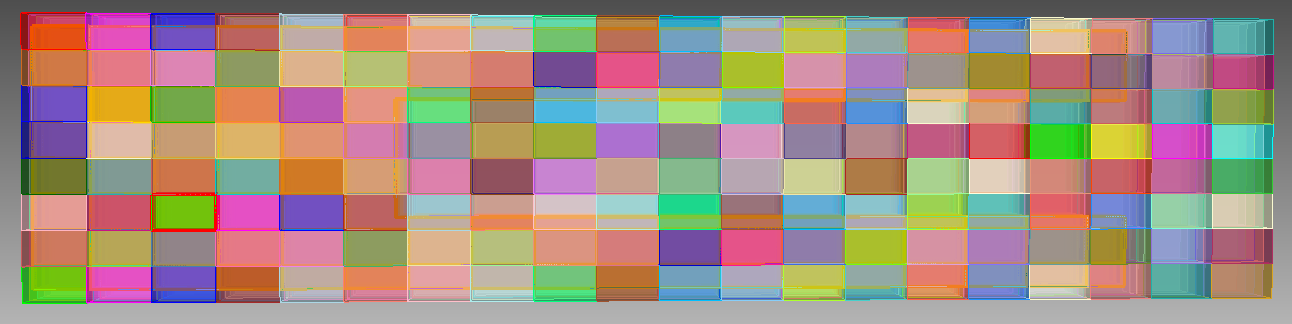
\includegraphics[scale=0.12]{figs/box_target_split_trelis.png}
                \end{figure}
                \begin{figure}
                        \centering
                        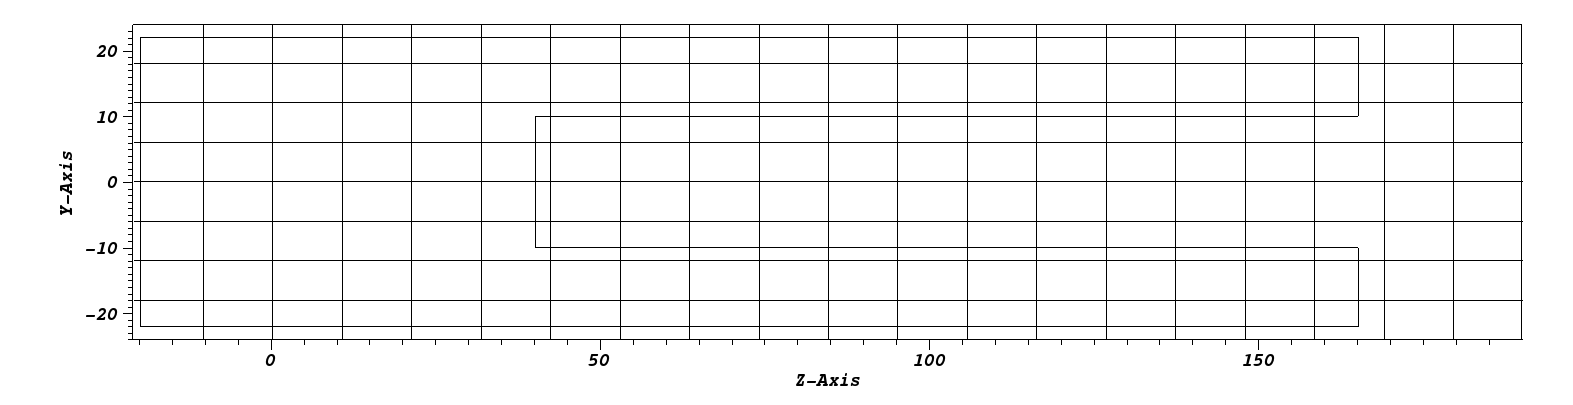
\includegraphics[scale=0.11]{figs/box_target_split_nograveyard.png}
                \end{figure}
	\begin{itemize}
		\item{Geometry split to align with the mesh used in mesh workflow}
		\item{1024 volumes. 480 mercury volumes and 544 steel volumes}
	\end{itemize}

        \column{.01\textwidth}
        \rule{.1mm}{.7\textheight}

        \column{0.49\textwidth}
	\textbf{Mesh Workflow}
                \begin{figure}
                        \centering
                        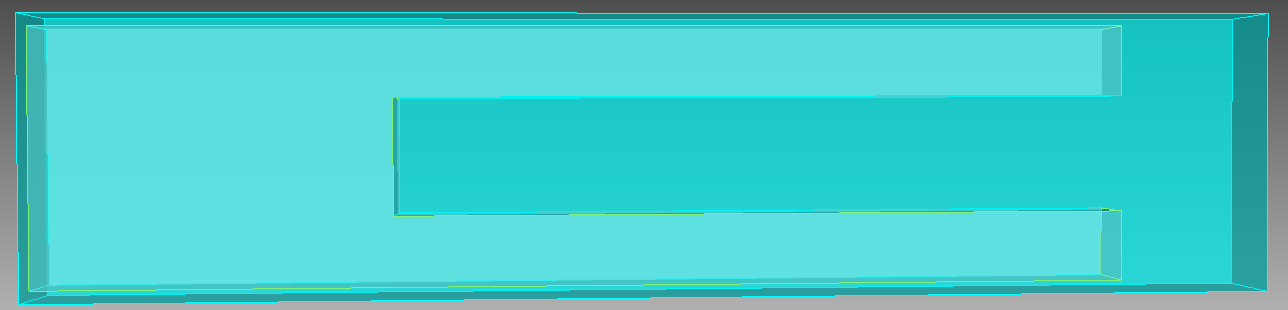
\includegraphics[scale=0.12]{figs/box_target_trelis.png}
                \end{figure}
                \begin{figure}
                        \centering
                        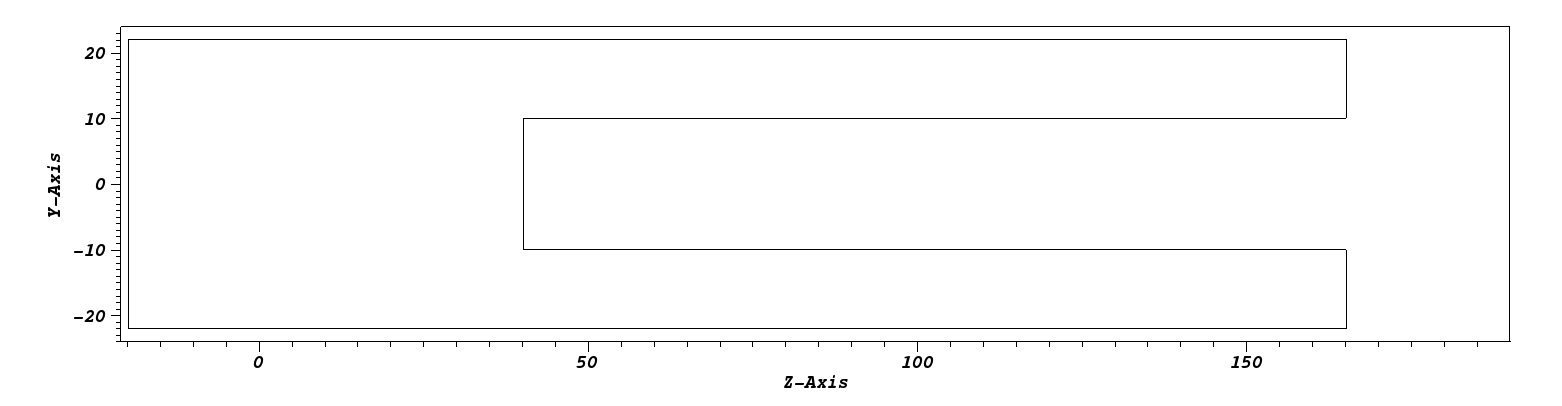
\includegraphics[scale=0.11]{figs/box_target_nograveyard.png}
                \end{figure}
	\begin{itemize}
		\item{Outer volume: steel}
		\item{Inner volume: mercury}
		\item{Mesh: 4x8x20}
	\end{itemize}
\end{columns}
\end{frame}

%%%%%%%% SLIDE %%%%%%%%%%
\begin{frame}{Neutron Transport}
\begin{columns}[T]
        \column{0.49\textwidth}
	\textbf{Cell Workflow}
	\begin{itemize}[<+->]
		\item<2->{Flux for each volume}
		\item<3->{Nuclide information for each volume}
	\end{itemize}

        \column{.01\textwidth}
        \rule{.1mm}{.7\textheight}

        \column{0.49\textwidth}
	\textbf{Mesh Workflow}
	\begin{itemize}[<+->]
		\item<2->{Flux in mesh over the full geometry (mesh size: 4x8x20)}
		\item<3->{Nuclide information for mercury material in mesh 4x8x20}
		\item<4->{Nuclide information for steel material in mesh 4x8x20}
	\end{itemize}
\end{columns}
\end{frame}

%%%%%%%% SLIDE %%%%%%%%%%
\begin{frame}{Activation}
\begin{columns}[T]
        \column{0.49\textwidth}
        \textbf{Cell Workflow}
        \begin{itemize}[<+->]
                \item<2->{Activate each volume}
        \end{itemize}

        \column{.01\textwidth}
        \rule{.1mm}{.7\textheight}

        \column{0.49\textwidth}
        \textbf{Mesh Workflow}
        \begin{itemize}[<+->]
                \item<2->{Activate 4x8x20 mesh with only mercury information}
                \item<3->{Activate 4x8x20 mesh with only steel information}
        \end{itemize}
\end{columns}
\end{frame}

\section{Photon Source}
%%%%%%%% SLIDE %%%%%%%%%%
\begin{frame}{Photon Source}
\begin{columns}[T]
        \column{0.49\textwidth}
        \textbf{Cell Workflow}
        \begin{itemize}[<+->]
                \item<2->{Two sources:}
			\begin{itemize}[<+->]
				\item<3->{All mercury volumes}
				\item<4->{All steel volumes}
			\end{itemize}
		\item<5->{3 sdef cards created per source due to number of volumes}
		\item<6->{3 sdef cards for mercury volumes}
		\item<6->{3 sdef cards for steel volumes}
        \end{itemize}

        \column{.01\textwidth}
        \rule{.1mm}{.7\textheight}

        \column{0.49\textwidth}
        \textbf{Mesh Workflow}
        \begin{itemize}[<+->]
                \item<2->{Two sources:}
			\begin{itemize}[<+->]
				\item<3->{Mercury mesh}
				\item<4->{Steel mesh}
			\end{itemize}
        \end{itemize}
\end{columns}
\end{frame}

%%%%%%%% SLIDE %%%%%%%%%%
\begin{frame}{Photon Source Visualization}
	\begin{itemize}
		\item{A \textit{tmesh} tally used to visualize the source}
		\item{Mesh used in \textit{tmesh} tally aligns with neutron 
			transport mesh and material boundaries}
		\item{Each dot in the graphs represent the source value 
			in a mesh volume element of tmesh  }
	\end{itemize}
\end{frame}

%%%%%%%% SLIDE %%%%%%%%%%
\begin{frame}{Photon Source - Mercury}
\begin{columns}[T]
        \column{0.75\textwidth}
        \textbf{Cell Workflow}
        \begin{figure}
                \centering
                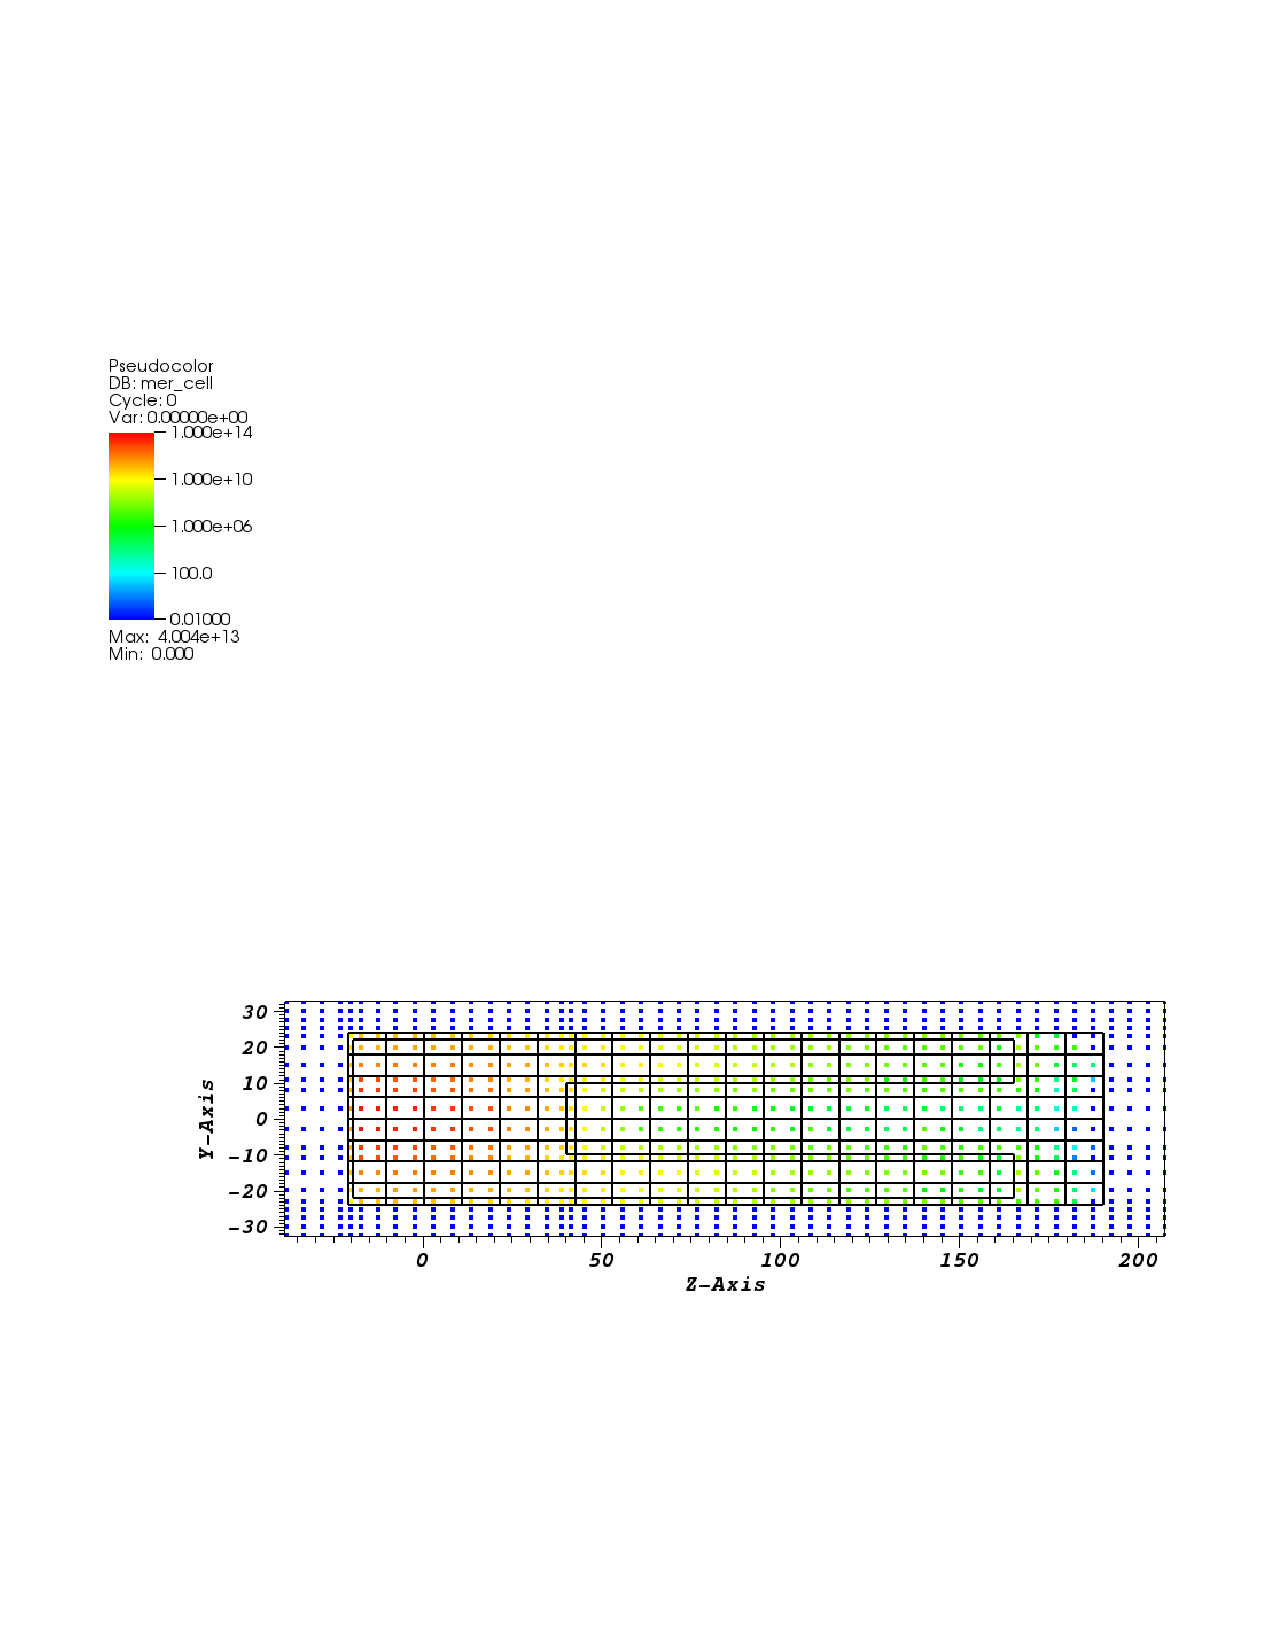
\includegraphics[scale=0.49,trim={2.5cm 6cm 1cm 16cm},clip]{figs/src_mer_cell.pdf}
        \end{figure}

        \column{0.25\textwidth}


        \begin{figure}
                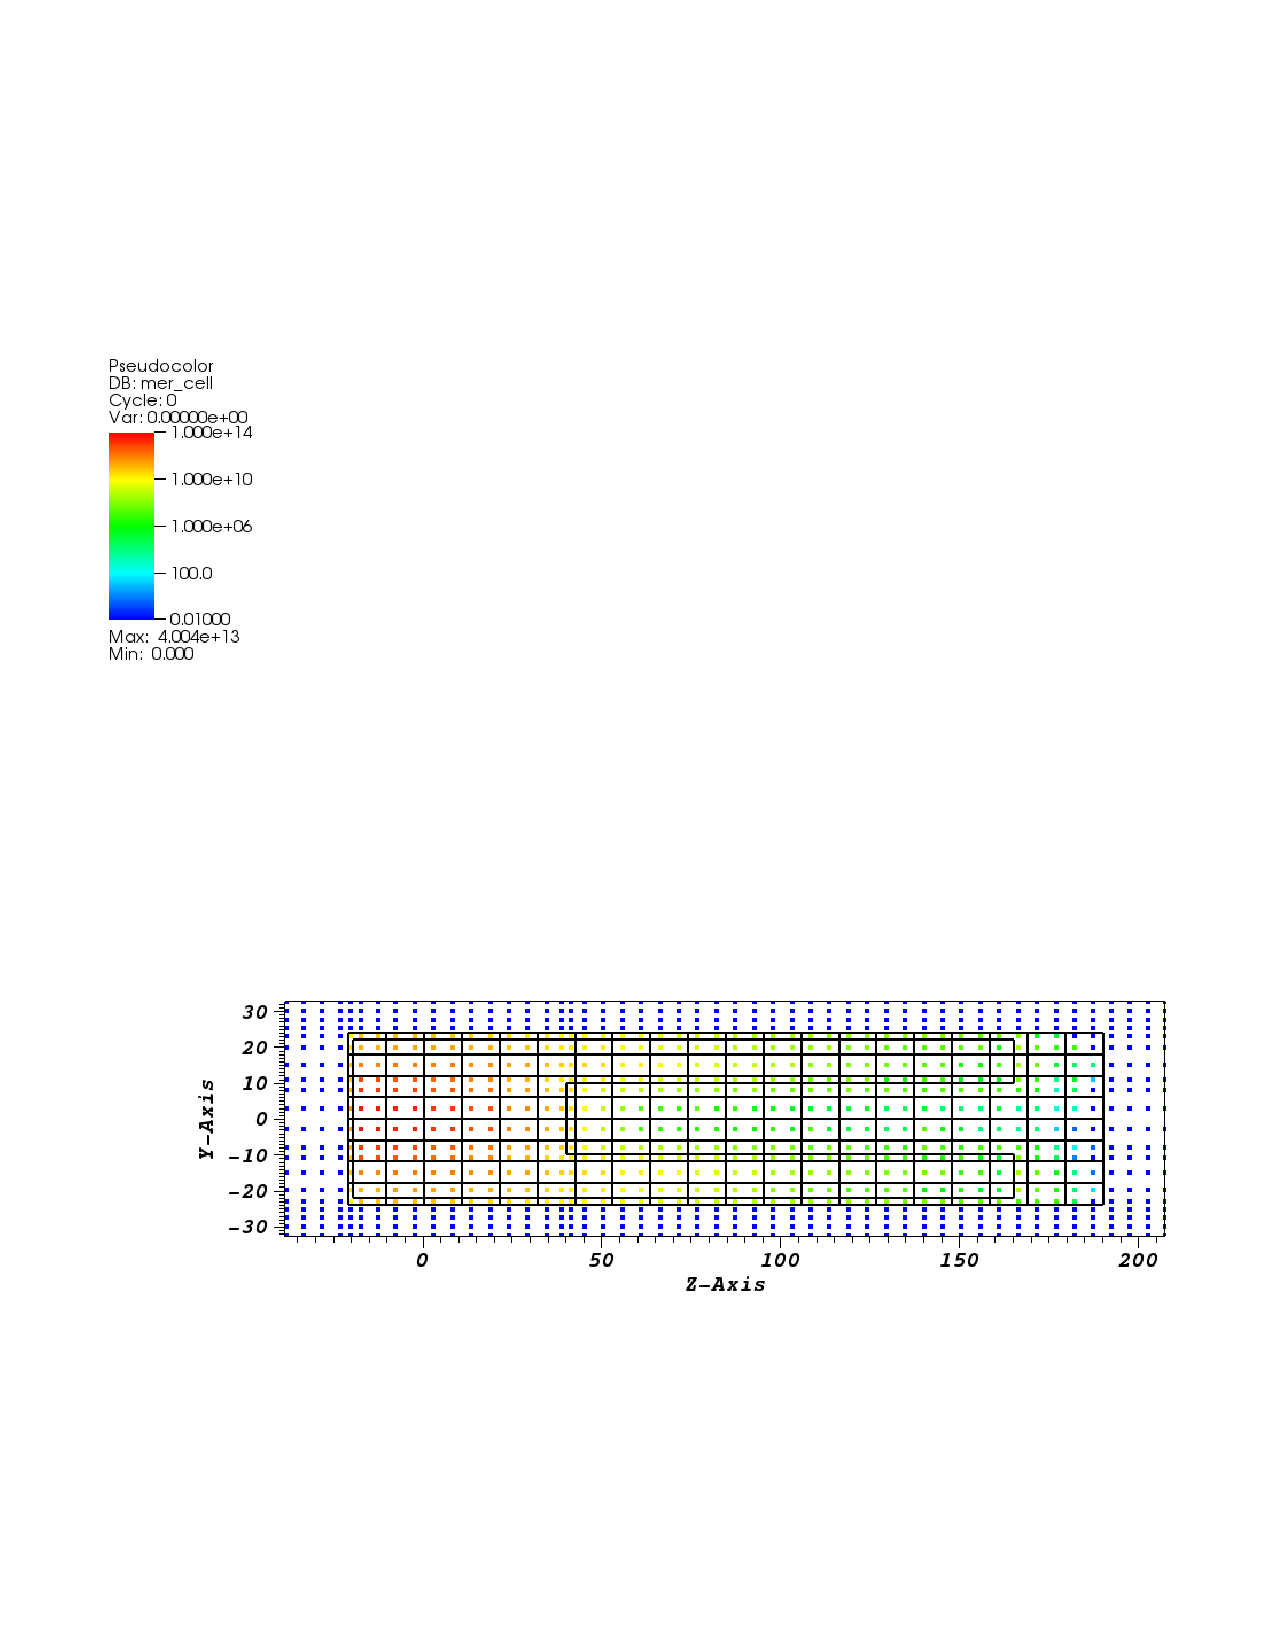
\includegraphics[scale=0.49,trim={1cm 16cm 9cm 5cm},clip]{figs/src_mer_cell.pdf}
        \end{figure}
\end{columns}

\begin{columns}[T]
        \column{0.75\textwidth}

        \textbf{Mesh Workflow}
        \begin{figure}
                \centering
                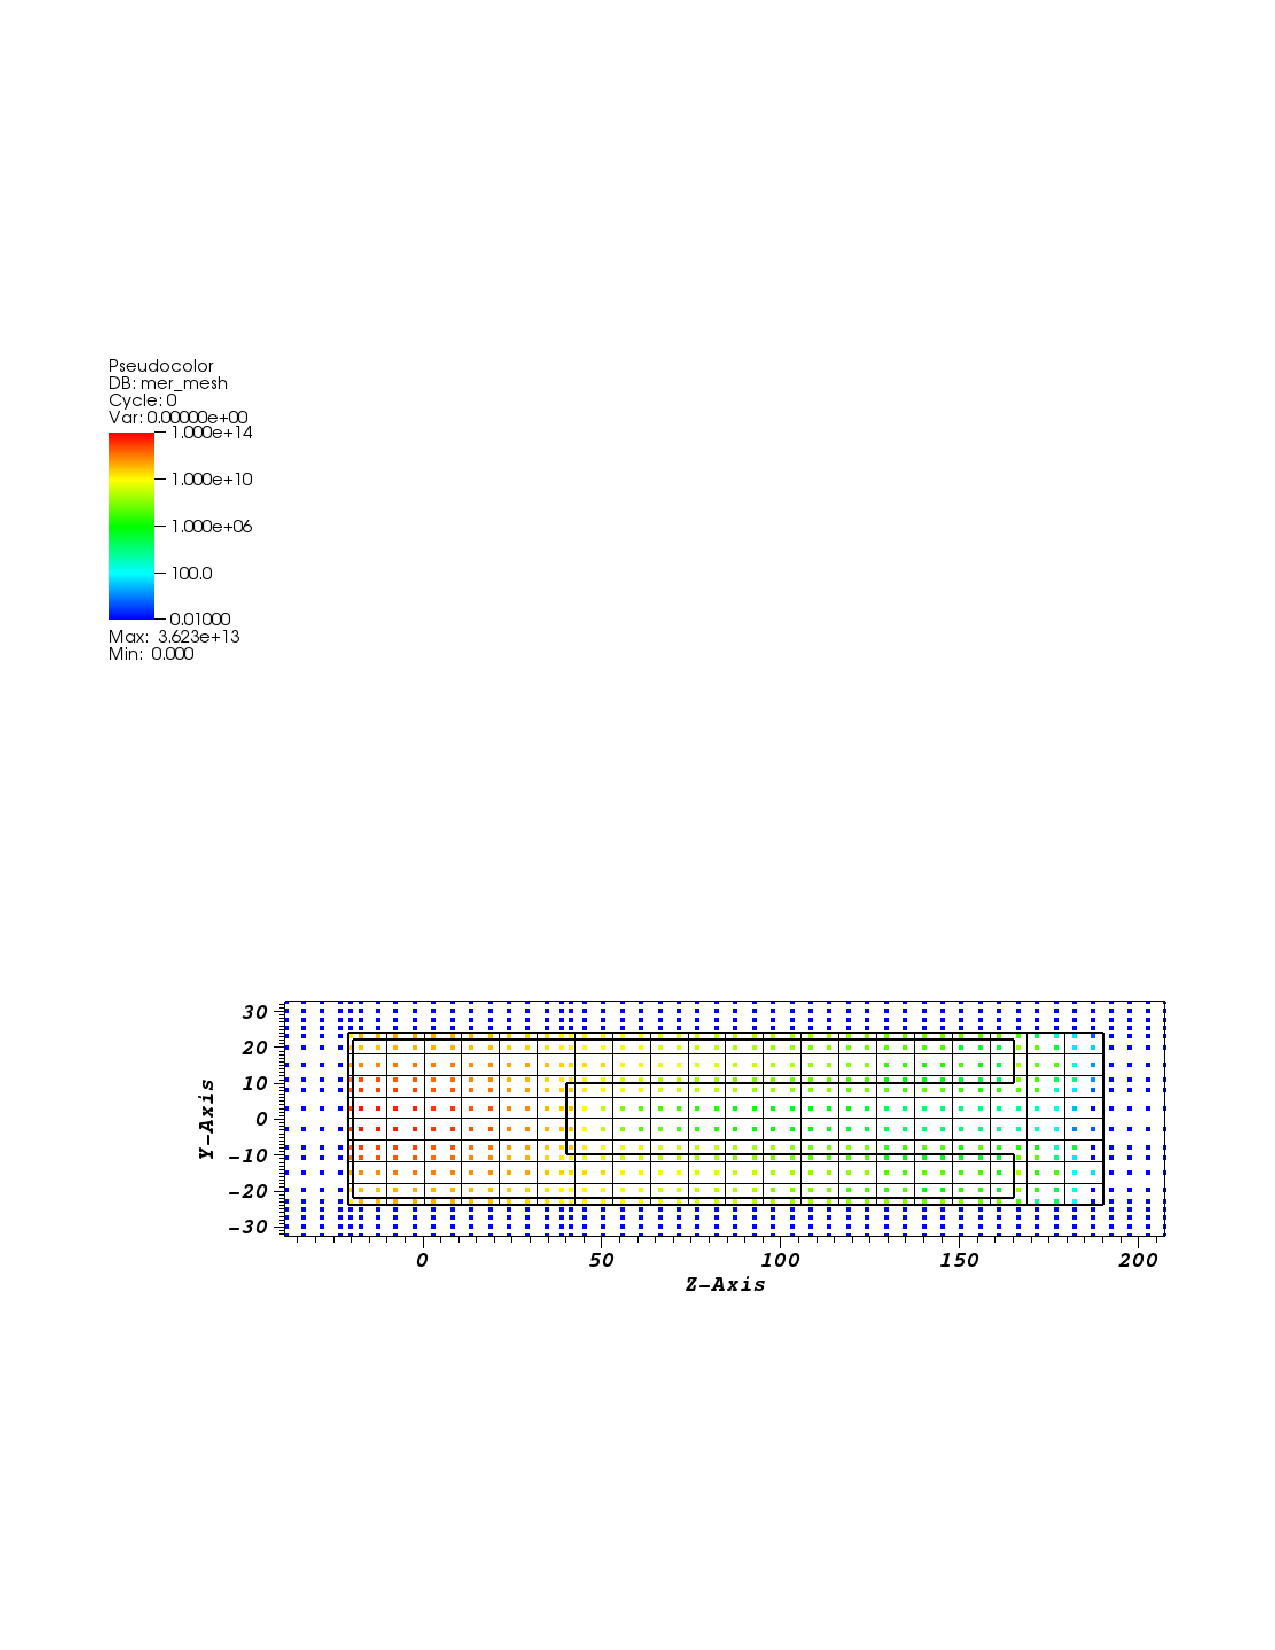
\includegraphics[scale=0.49,trim={2.5cm 6cm 1cm 16cm},clip]{figs/src_mer_mesh.pdf}
        \end{figure}
        \column{0.25\textwidth}

\end{columns}
\end{frame}

%%%%%%%% SLIDE %%%%%%%%%%
\begin{frame}{Source Ratio - Steel}

  \begin{columns}[T]
  \column{0.8\textwidth}
        \begin{figure}
                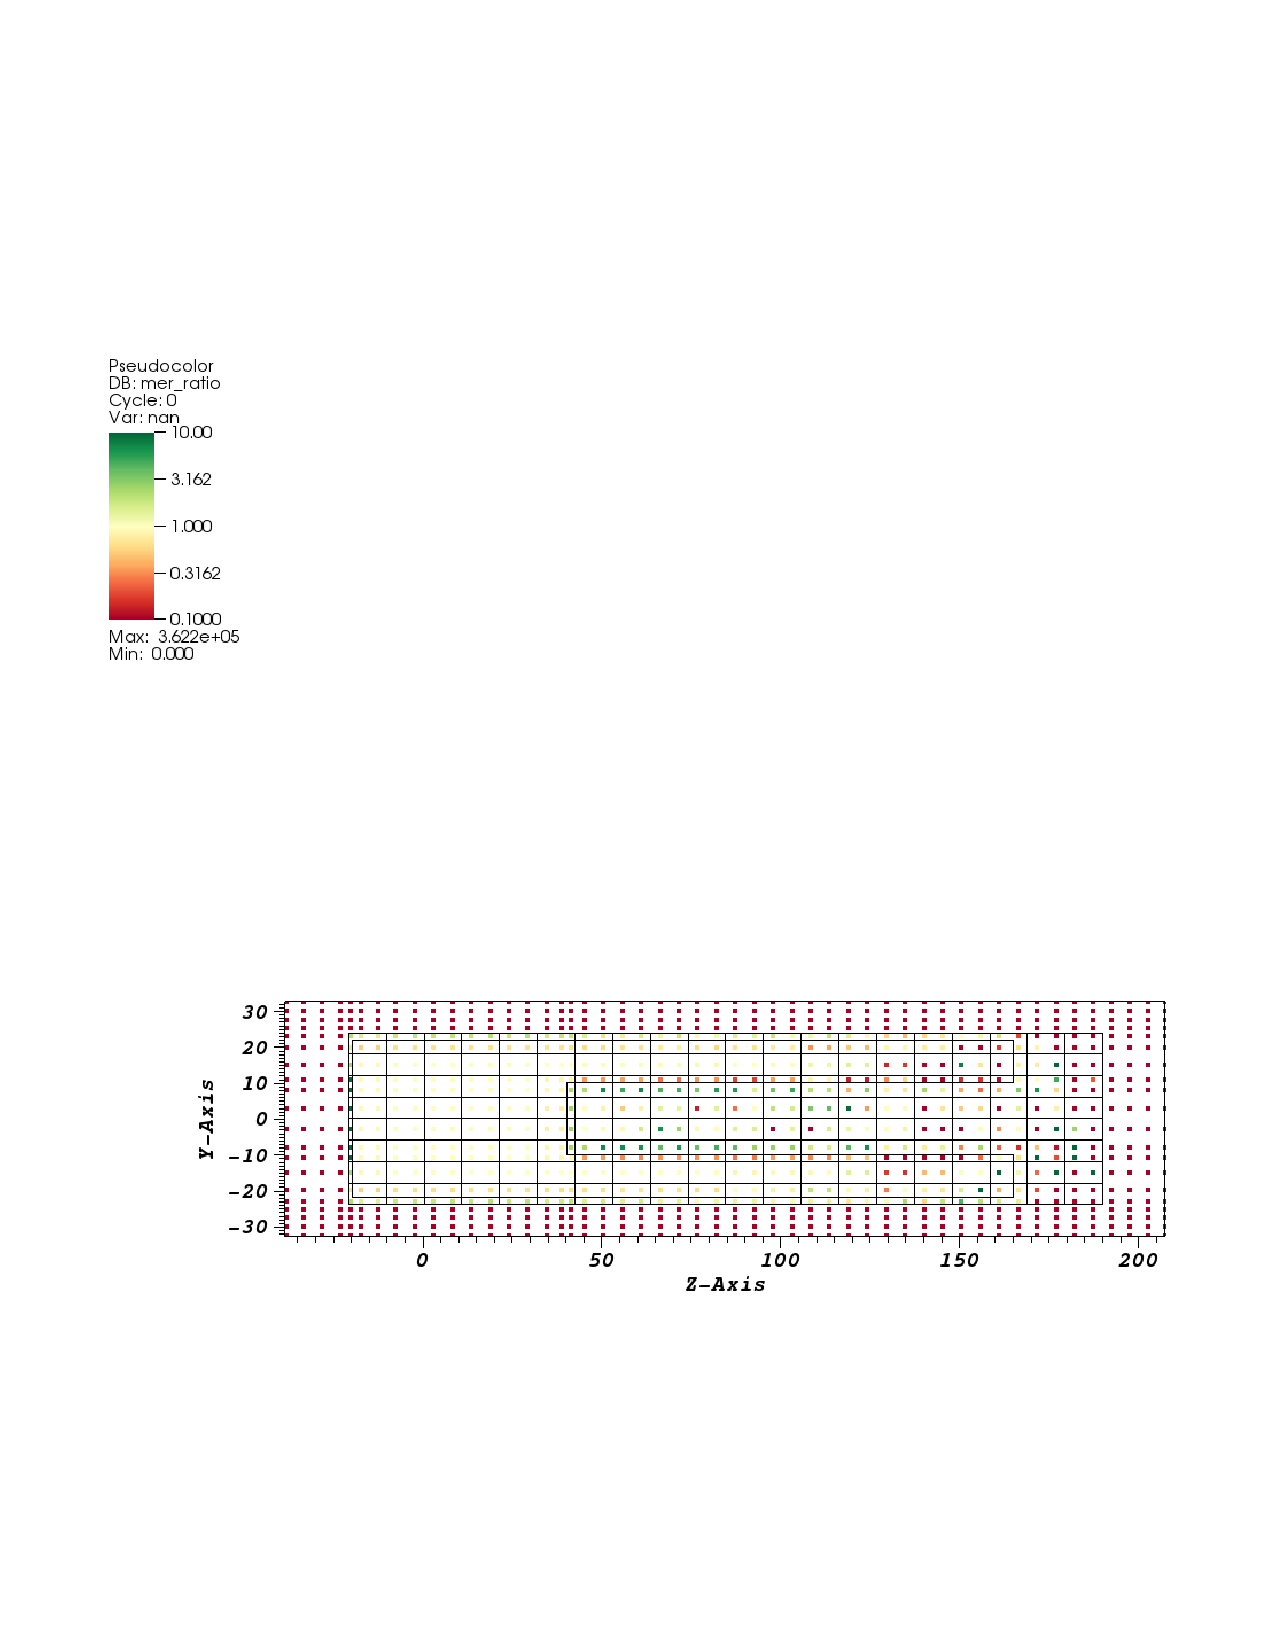
\includegraphics[scale=0.5,trim={2.5cm 6cm 1cm 15cm},clip]{figs/src_ratio_mer.pdf}
        \end{figure}

  \column{0.2\textwidth}
        \begin{figure}
                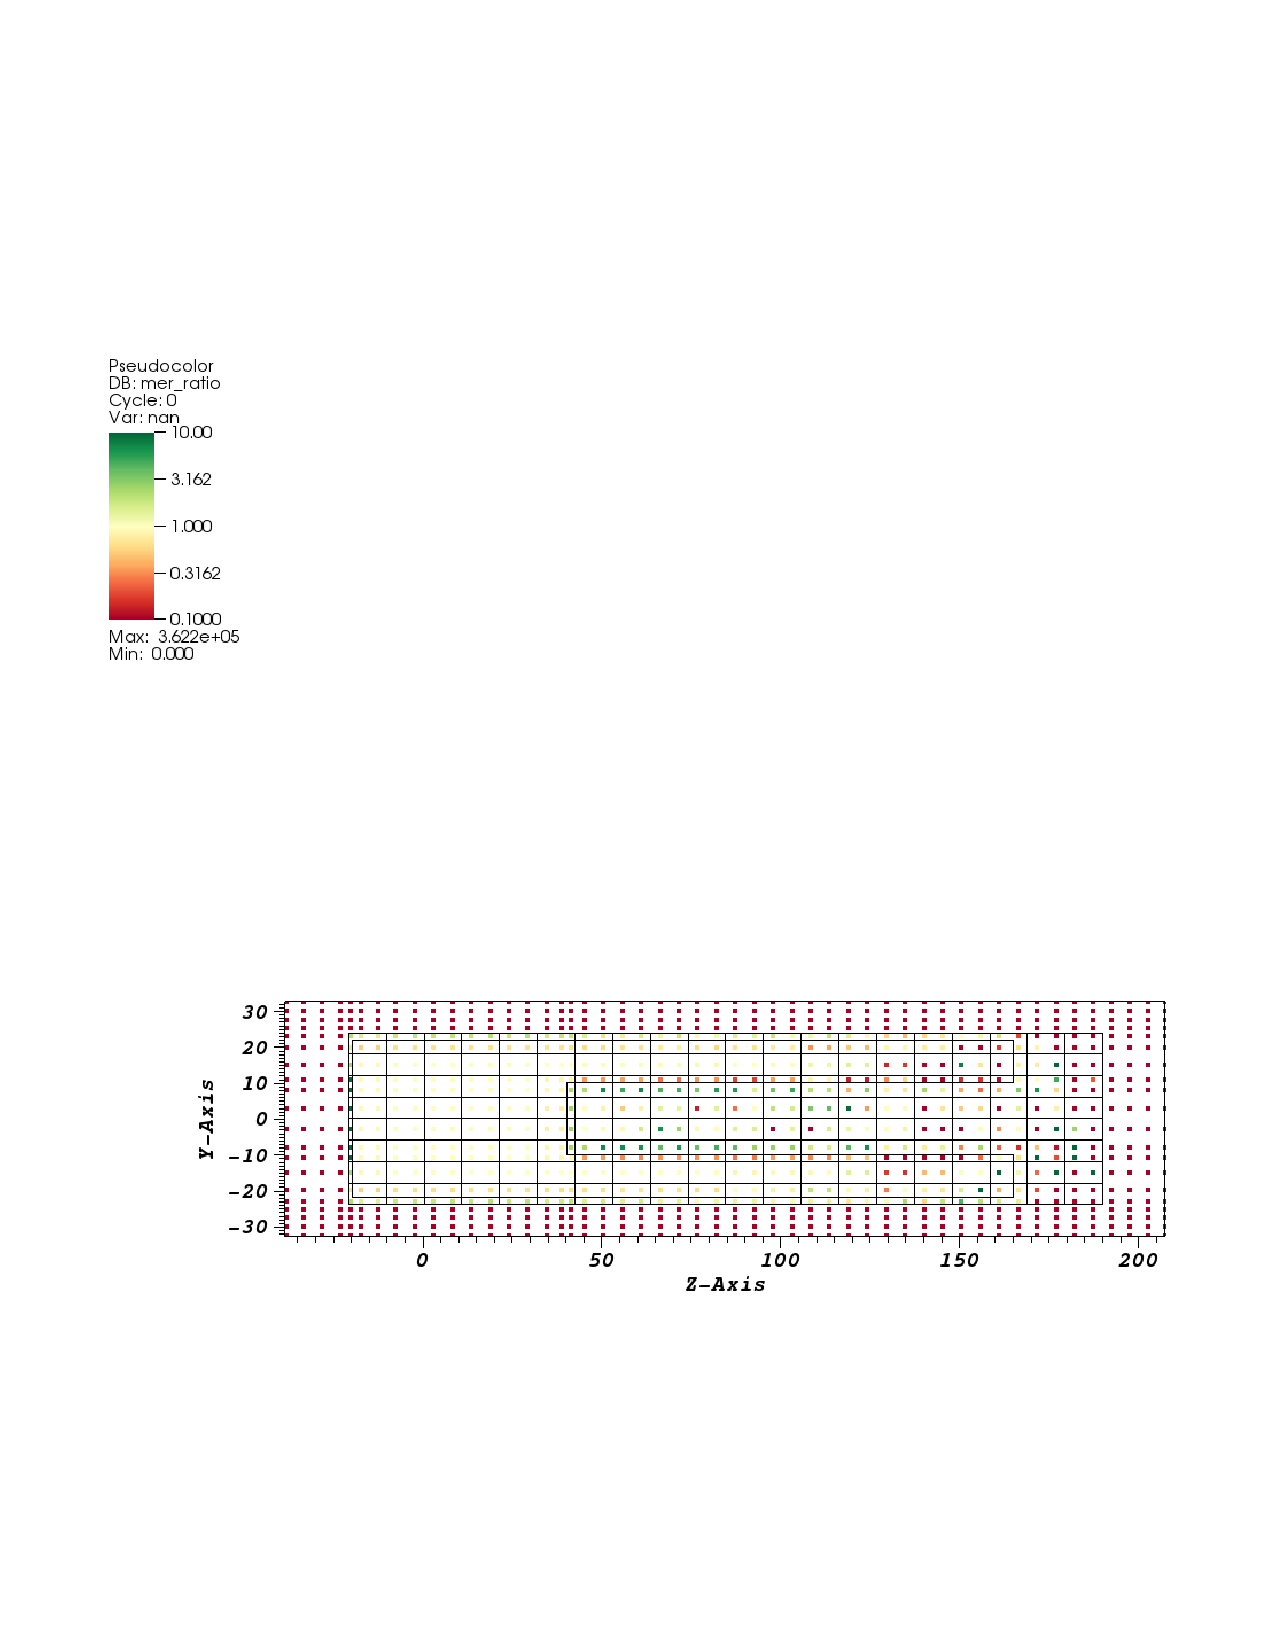
\includegraphics[scale=0.5,trim={1cm 16cm 9cm 5cm},clip]{figs/src_ratio_mer.pdf}
        % \end{flushleft}
        \end{figure}
  \end{columns}
\end{frame}

%%%%%%%% SLIDE %%%%%%%%%%
\begin{frame}{Photon Source - Steel}
\begin{columns}[T]
        \column{0.75\textwidth}
        \textbf{Cell Workflow}
        \begin{figure}
                \centering
                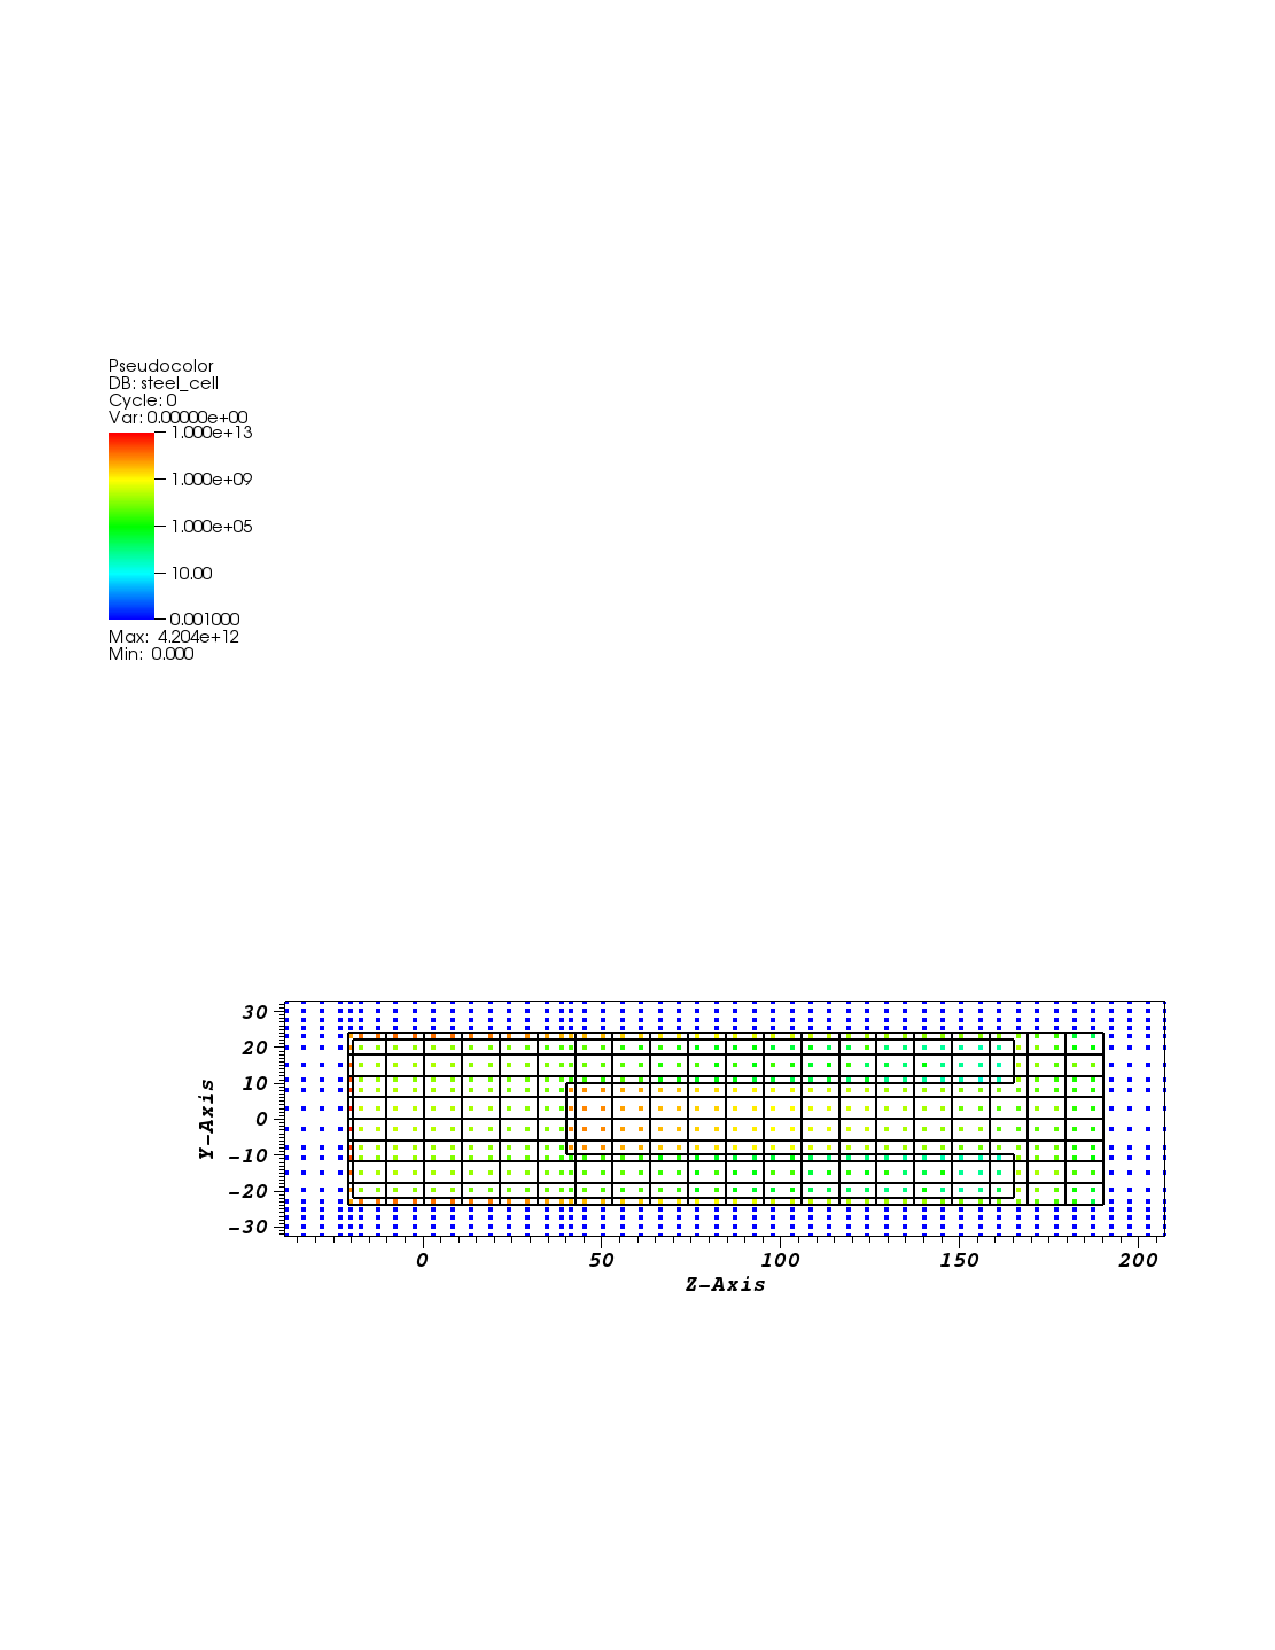
\includegraphics[scale=0.49,trim={2.5cm 6cm 1cm 16cm},clip]{figs/src_steel_cell.pdf}
        \end{figure}

        \column{0.25\textwidth}


        \begin{figure}
                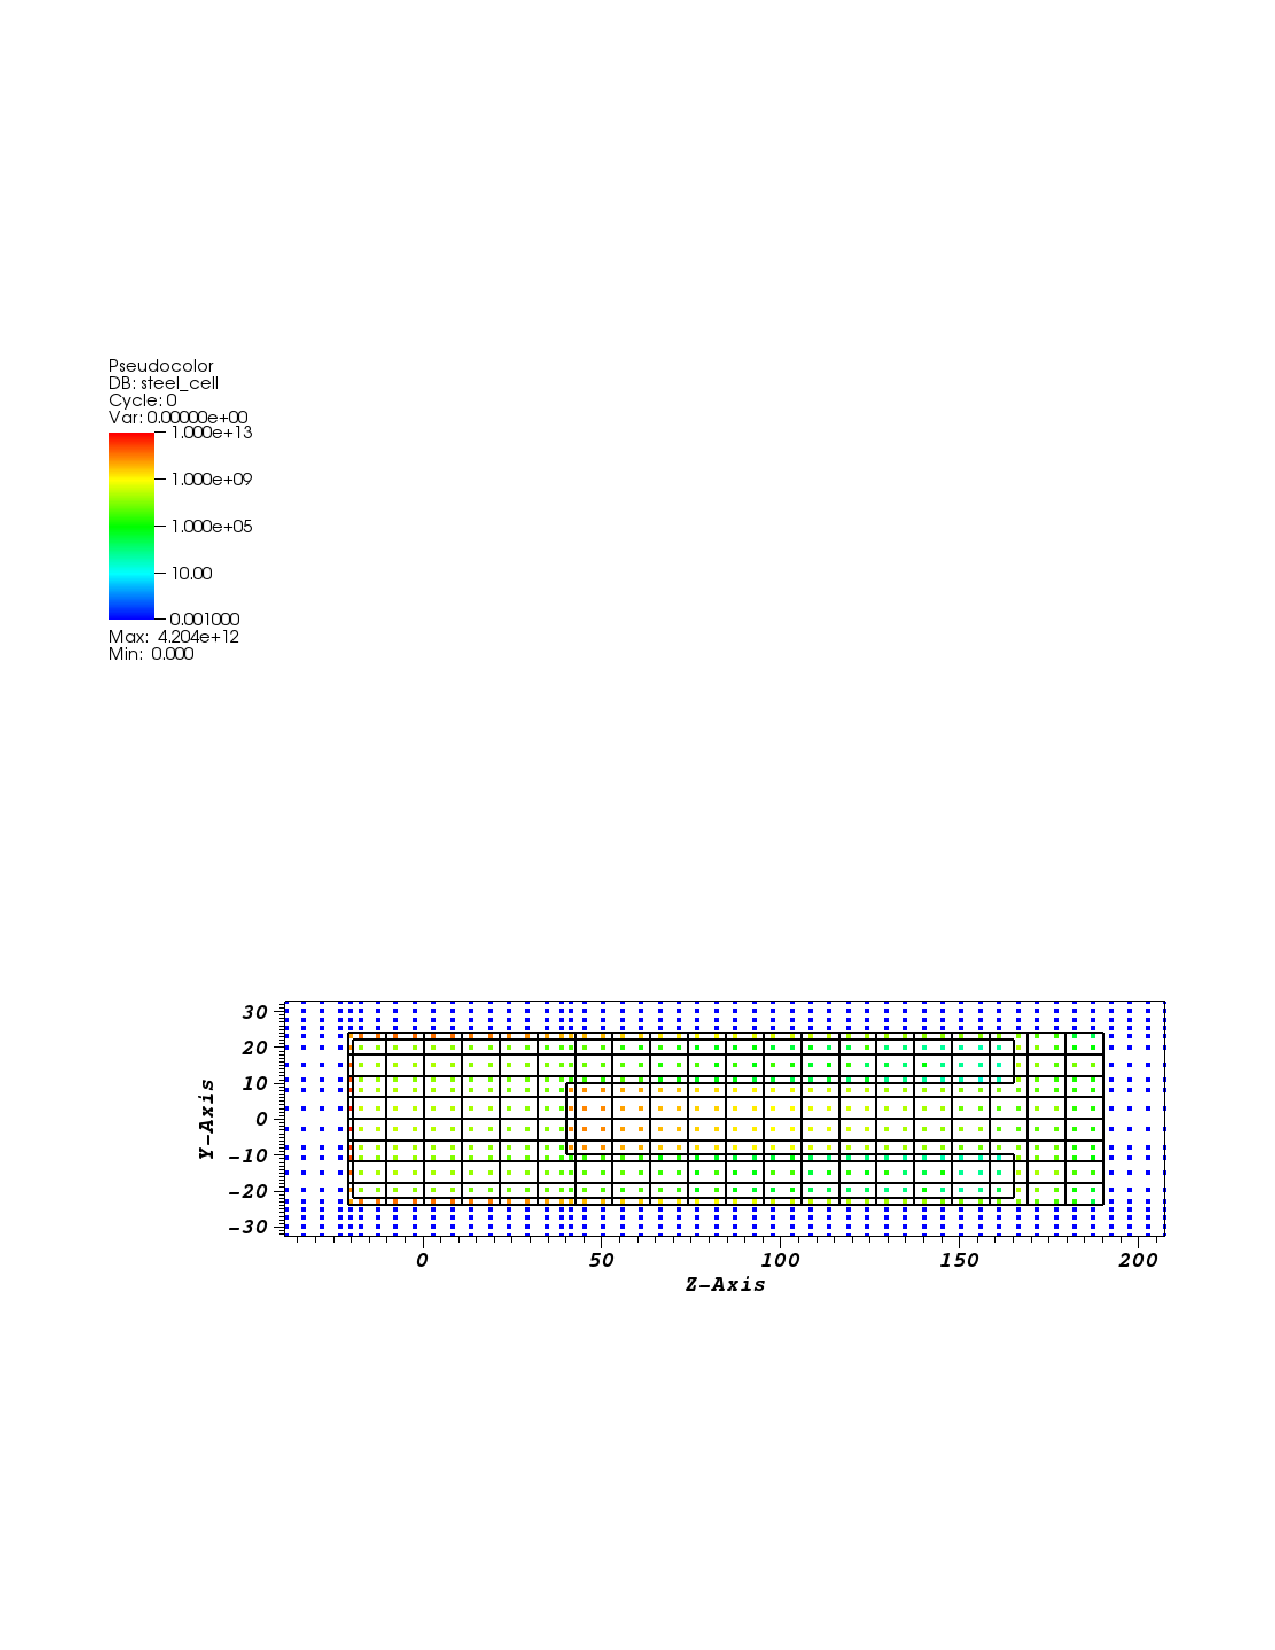
\includegraphics[scale=0.49,trim={1cm 16cm 9cm 5cm},clip]{figs/src_steel_cell.pdf}
        \end{figure}
\end{columns}

\begin{columns}[T]
        \column{0.75\textwidth}

        \textbf{Mesh Workflow}
        \begin{figure}
                \centering
                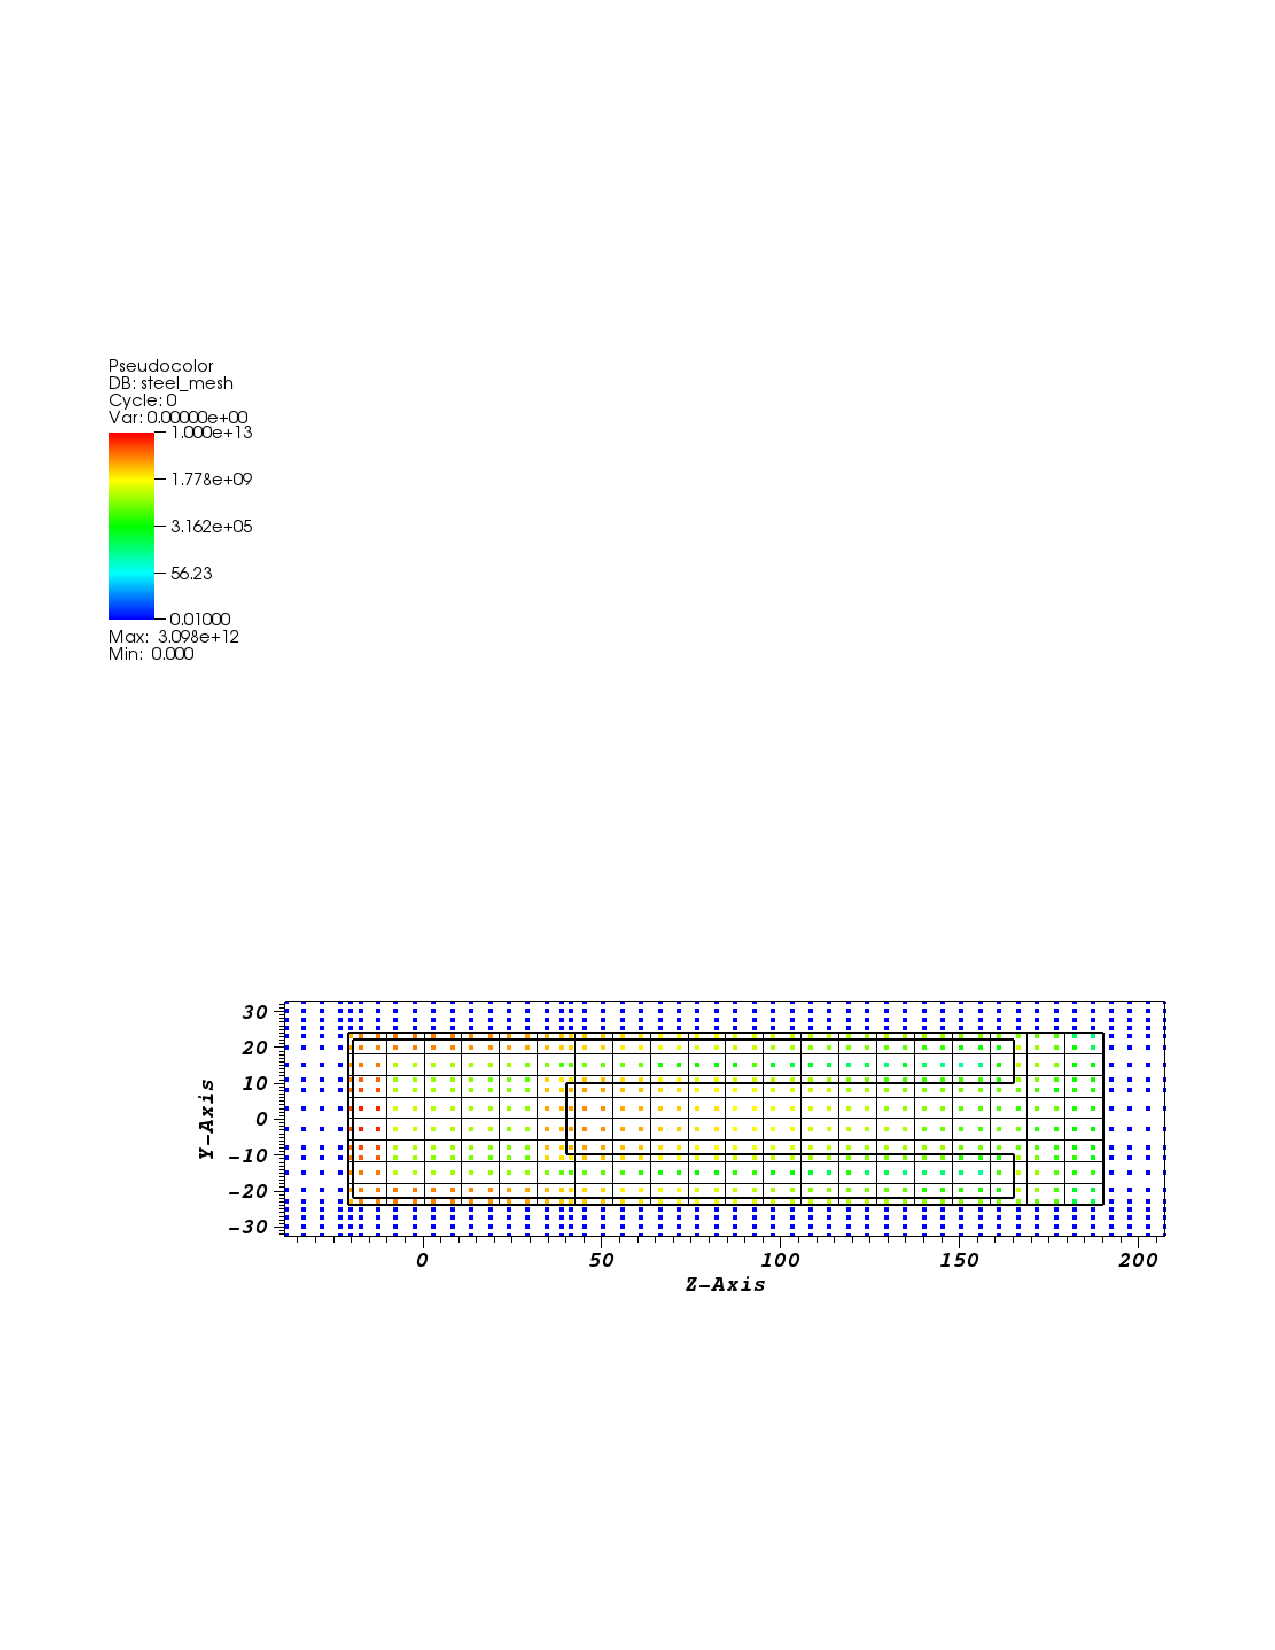
\includegraphics[scale=0.49,trim={2.5cm 6cm 1cm 16cm},clip]{figs/src_steel_mesh.pdf}
        \end{figure}
        \column{0.25\textwidth}

\end{columns}
\end{frame}

%%%%%%%% SLIDE %%%%%%%%%%
\begin{frame}{Source Ratio - Steel}

  \begin{columns}[T]
  \column{0.8\textwidth}
        \begin{figure}
                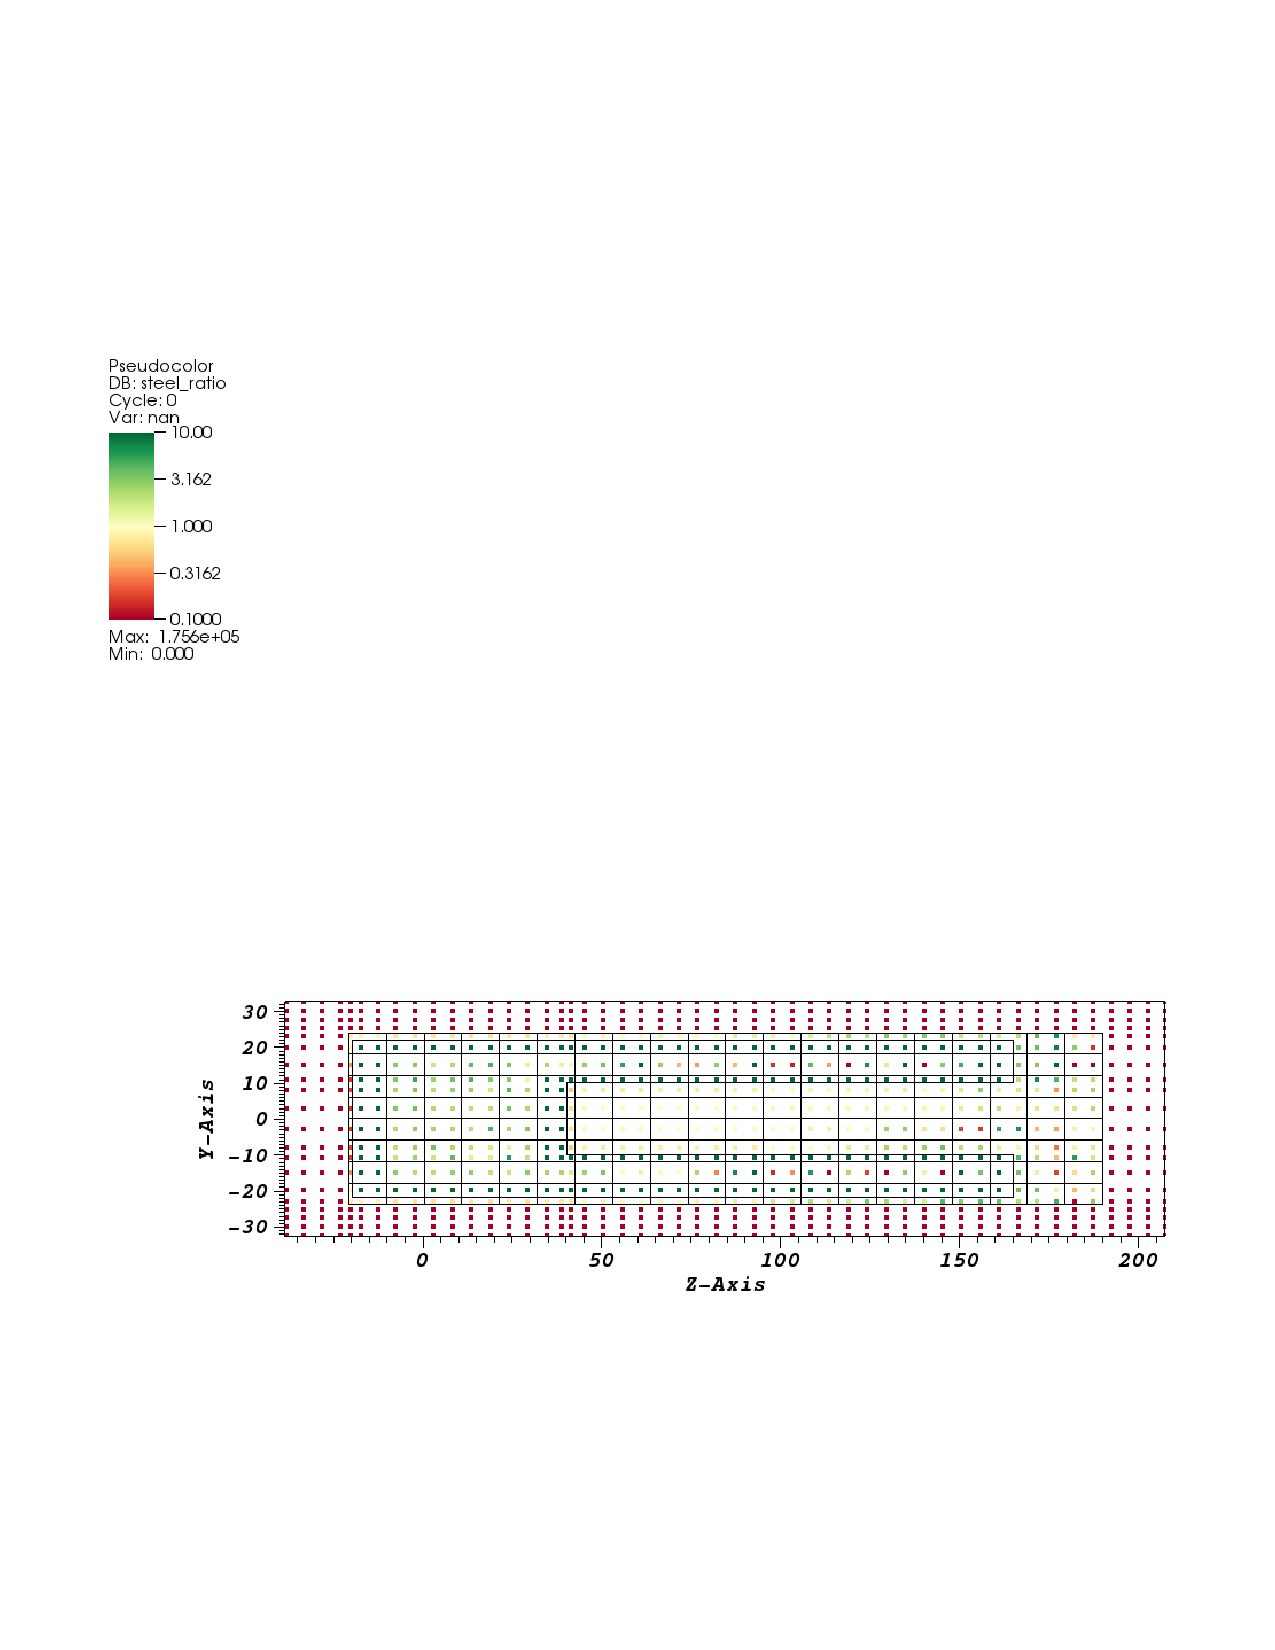
\includegraphics[scale=0.5,trim={2.5cm 6cm 1cm 15cm},clip]{figs/src_ratio_steel.pdf}
        \end{figure}

  \column{0.2\textwidth}
        \begin{figure}
                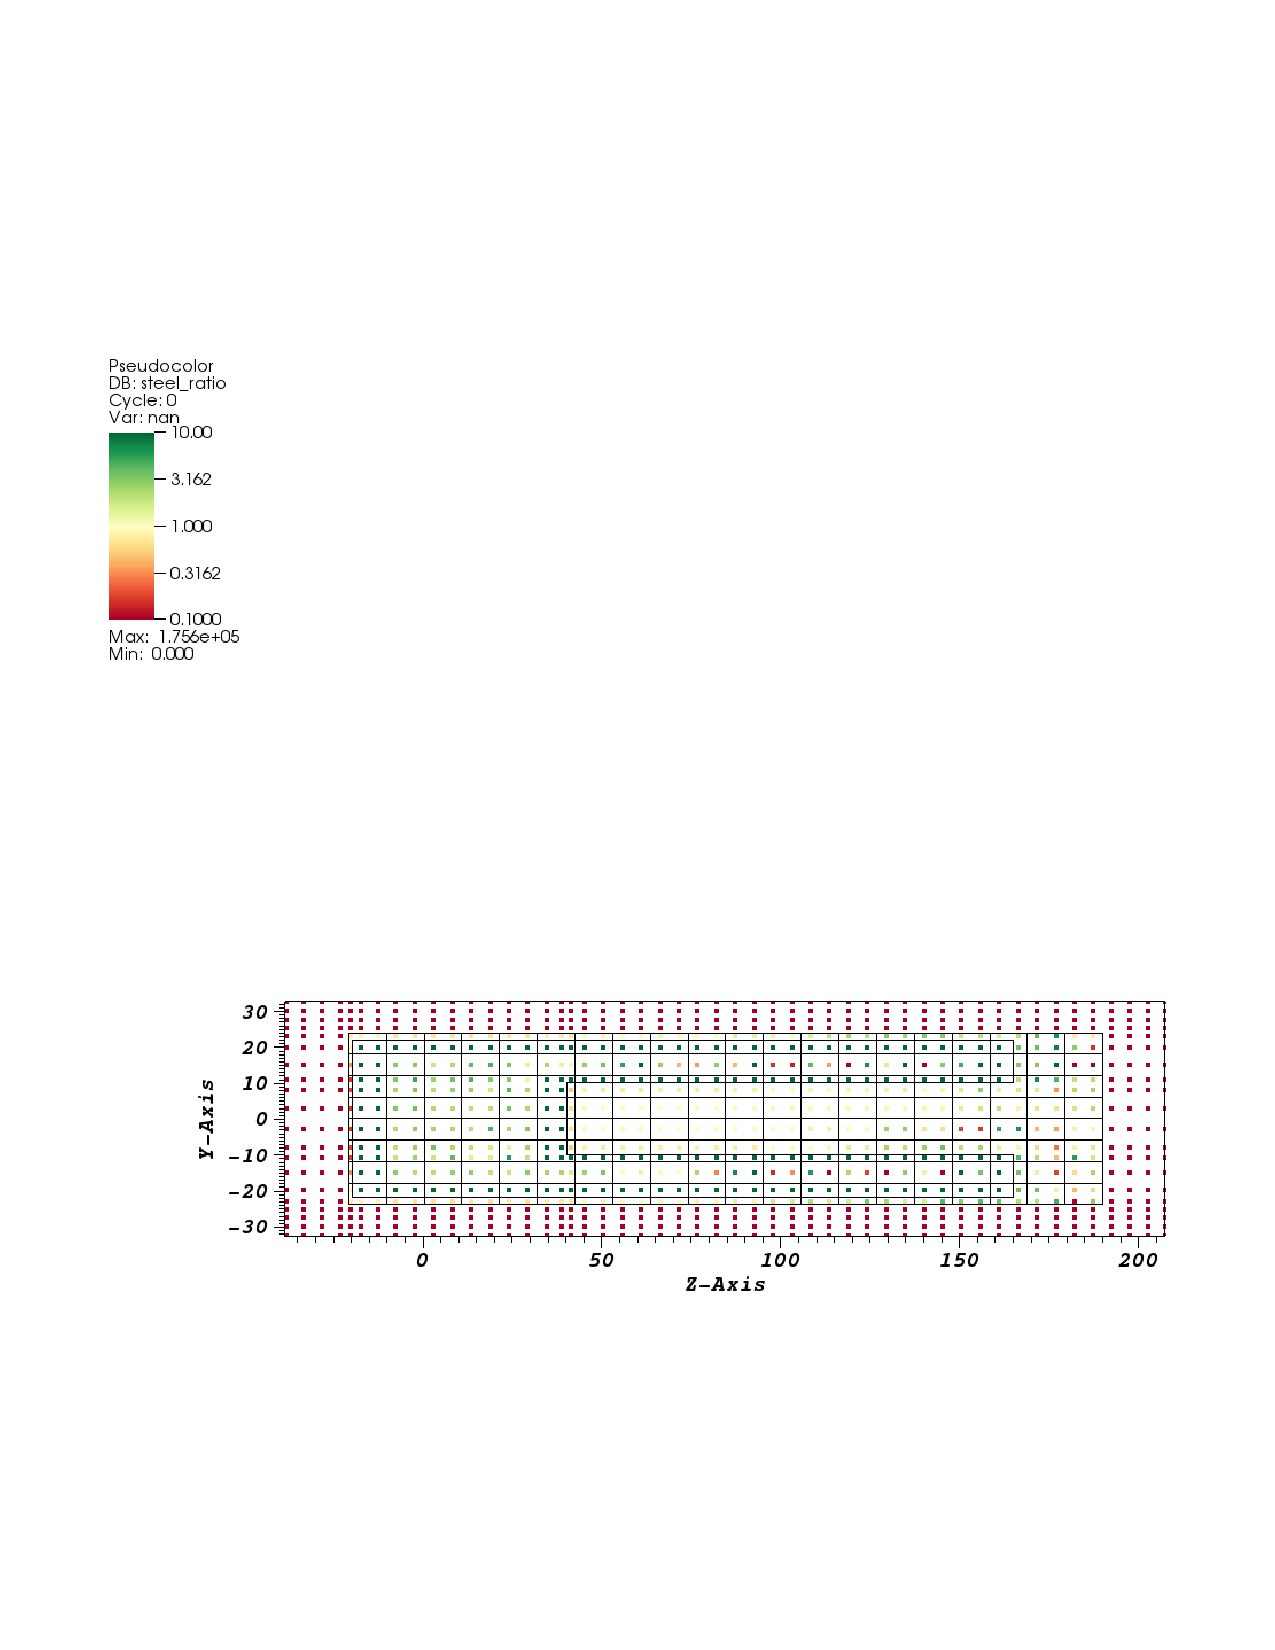
\includegraphics[scale=0.5,trim={1cm 16cm 9cm 5cm},clip]{figs/src_ratio_steel.pdf}
        \end{figure}
  \end{columns}
\end{frame}

\section{Dose Rates - Partially Voided Geometry}

\begin{frame}{Dose Rates: Mercury Source, Void Steel Volumes}
\begin{columns}[T]
        \column{0.8\textwidth}
        \textbf{Cell Workflow}
        \begin{figure}
                \centering
                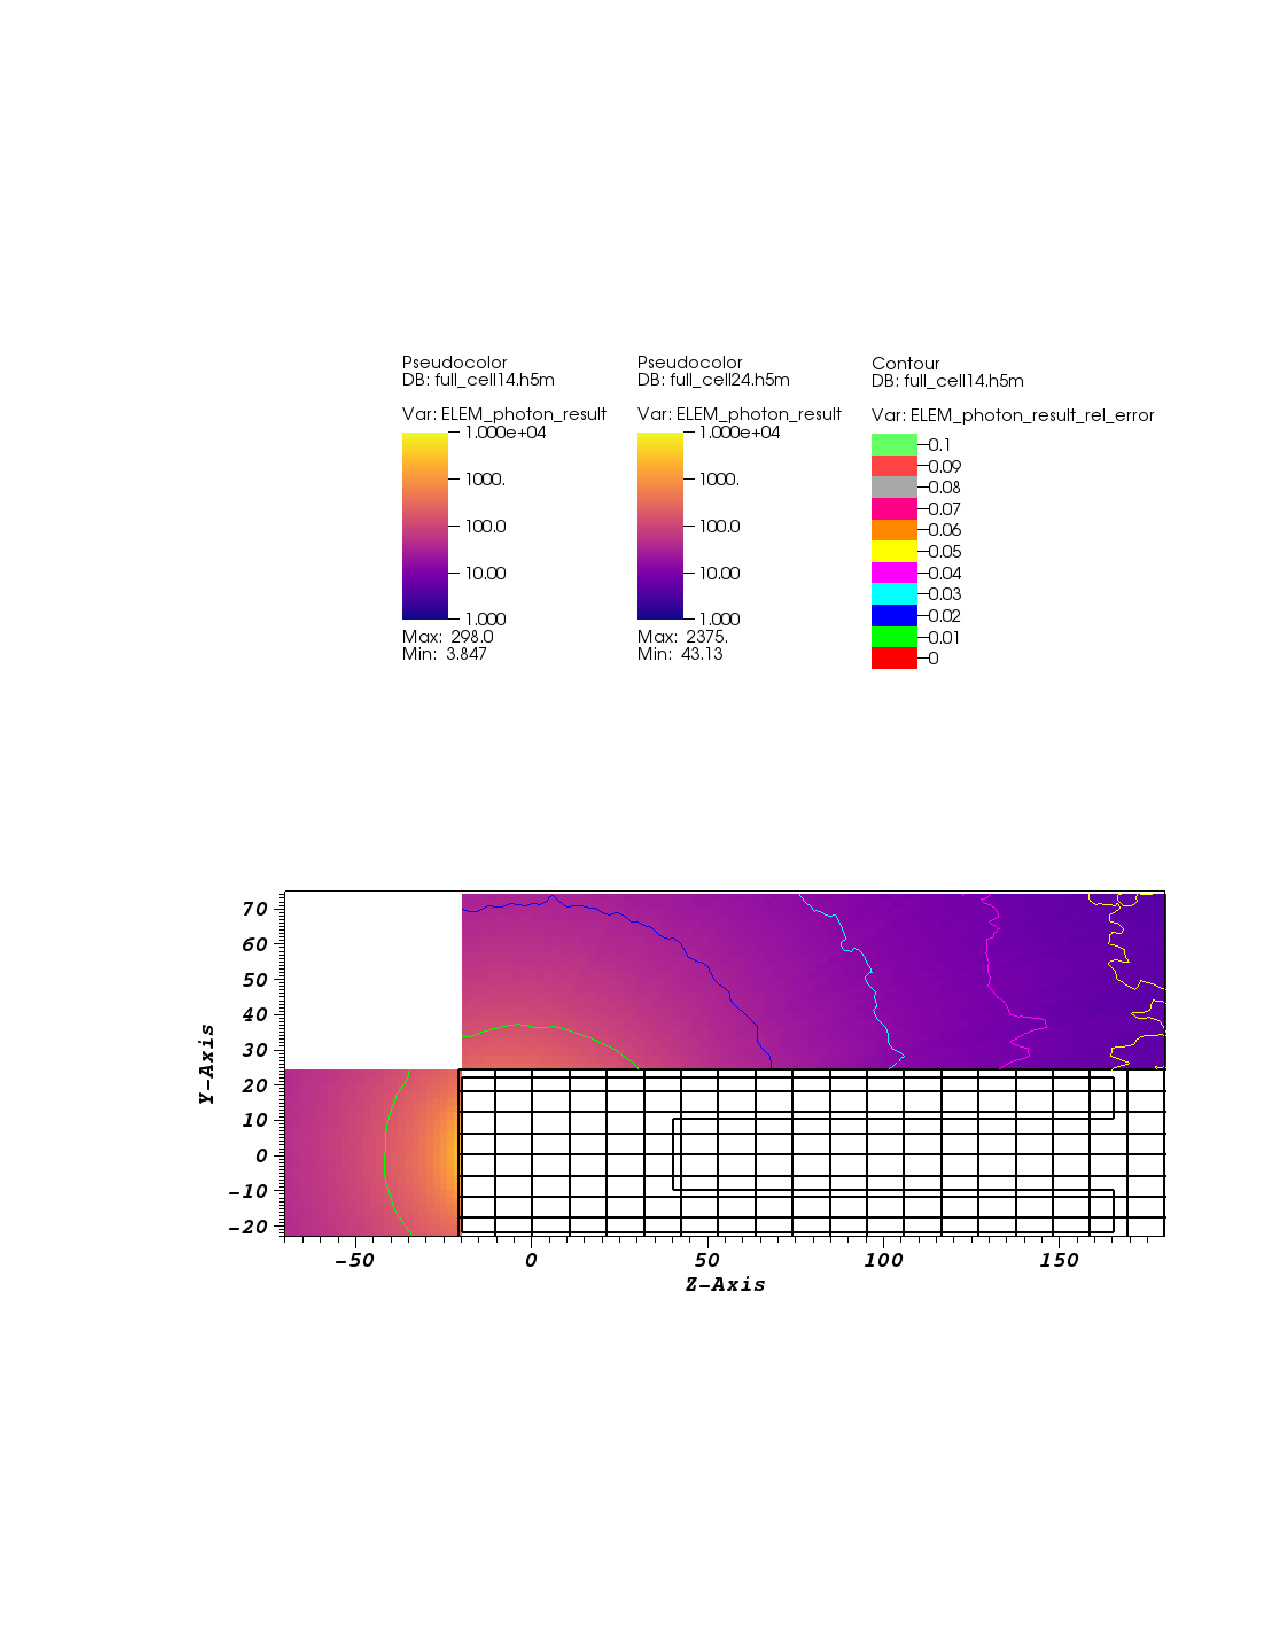
\includegraphics[scale=0.49,trim={2.5cm 6cm 1cm 15cm},clip]{figs/dose_mer_cell_void.pdf}
        \end{figure}

        \column{0.2\textwidth}

	\tiny{* thick line = geom} \\
	\tiny{* thin line = src mesh}

        \begin{figure}
                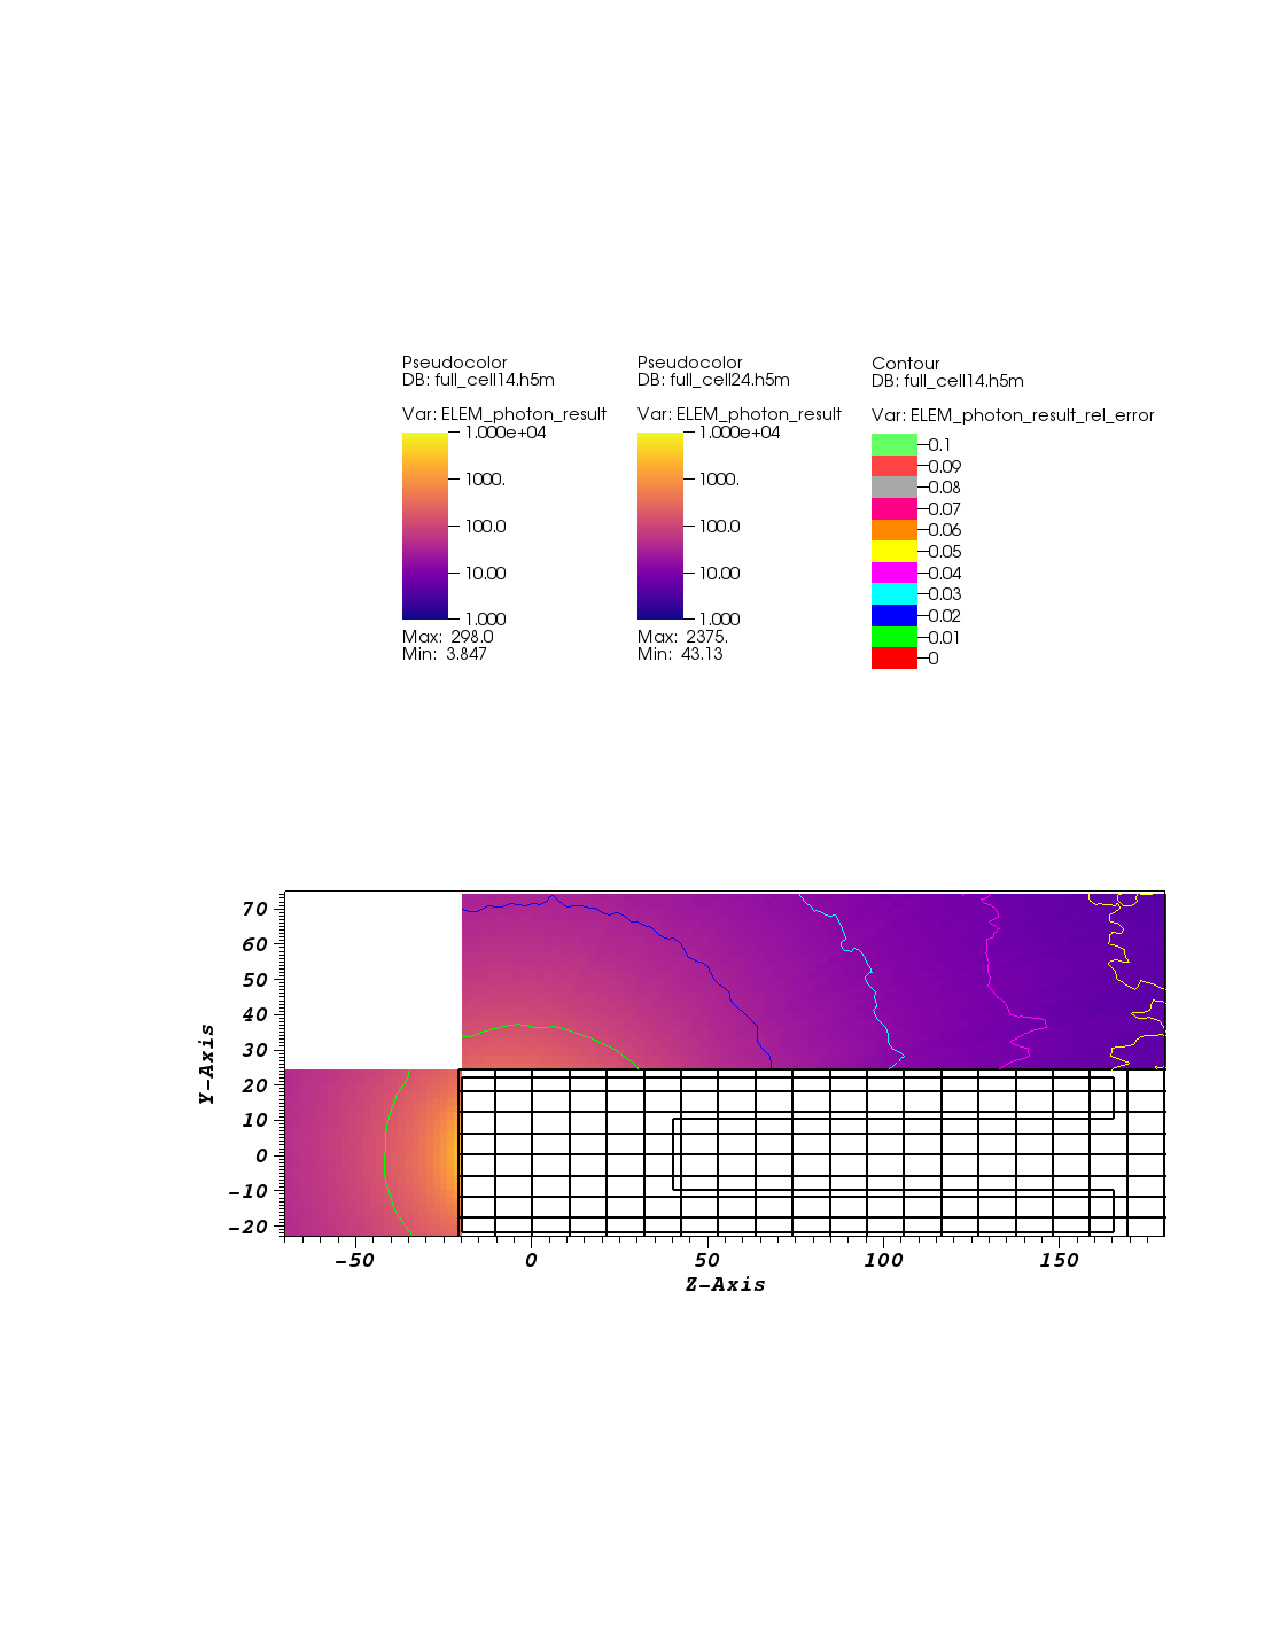
\includegraphics[scale=0.49,trim={6.75cm 16.5cm 11cm 6cm},clip]{figs/dose_mer_cell_void.pdf}
        \end{figure}
\end{columns}

\begin{columns}[T]
        \column{0.8\textwidth}

        \textbf{Mesh Workflow}
        \begin{figure}
                \centering
                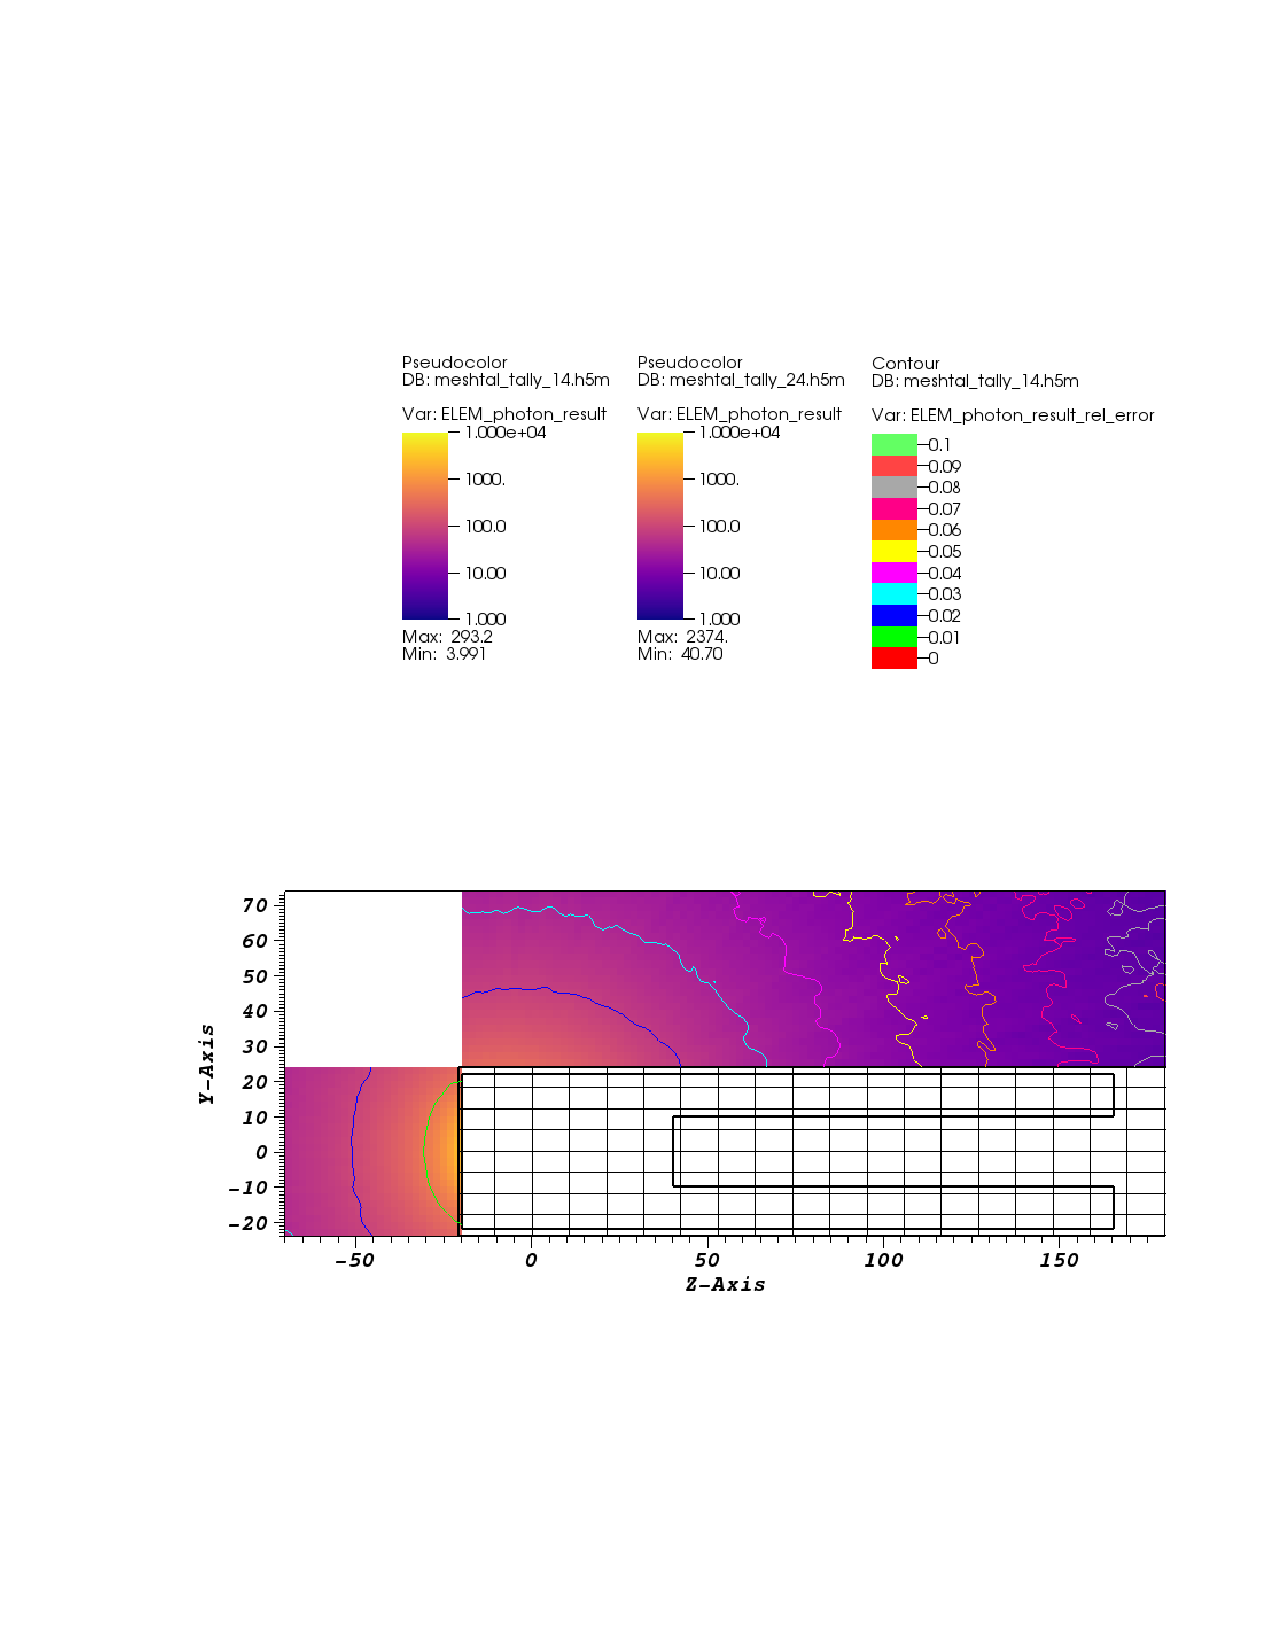
\includegraphics[scale=0.49,trim={2.5cm 6cm 1cm 15cm},clip]{figs/dose_mer_mesh_void.pdf}
        \end{figure}

        \column{0.2\textwidth}
        \begin{figure}
                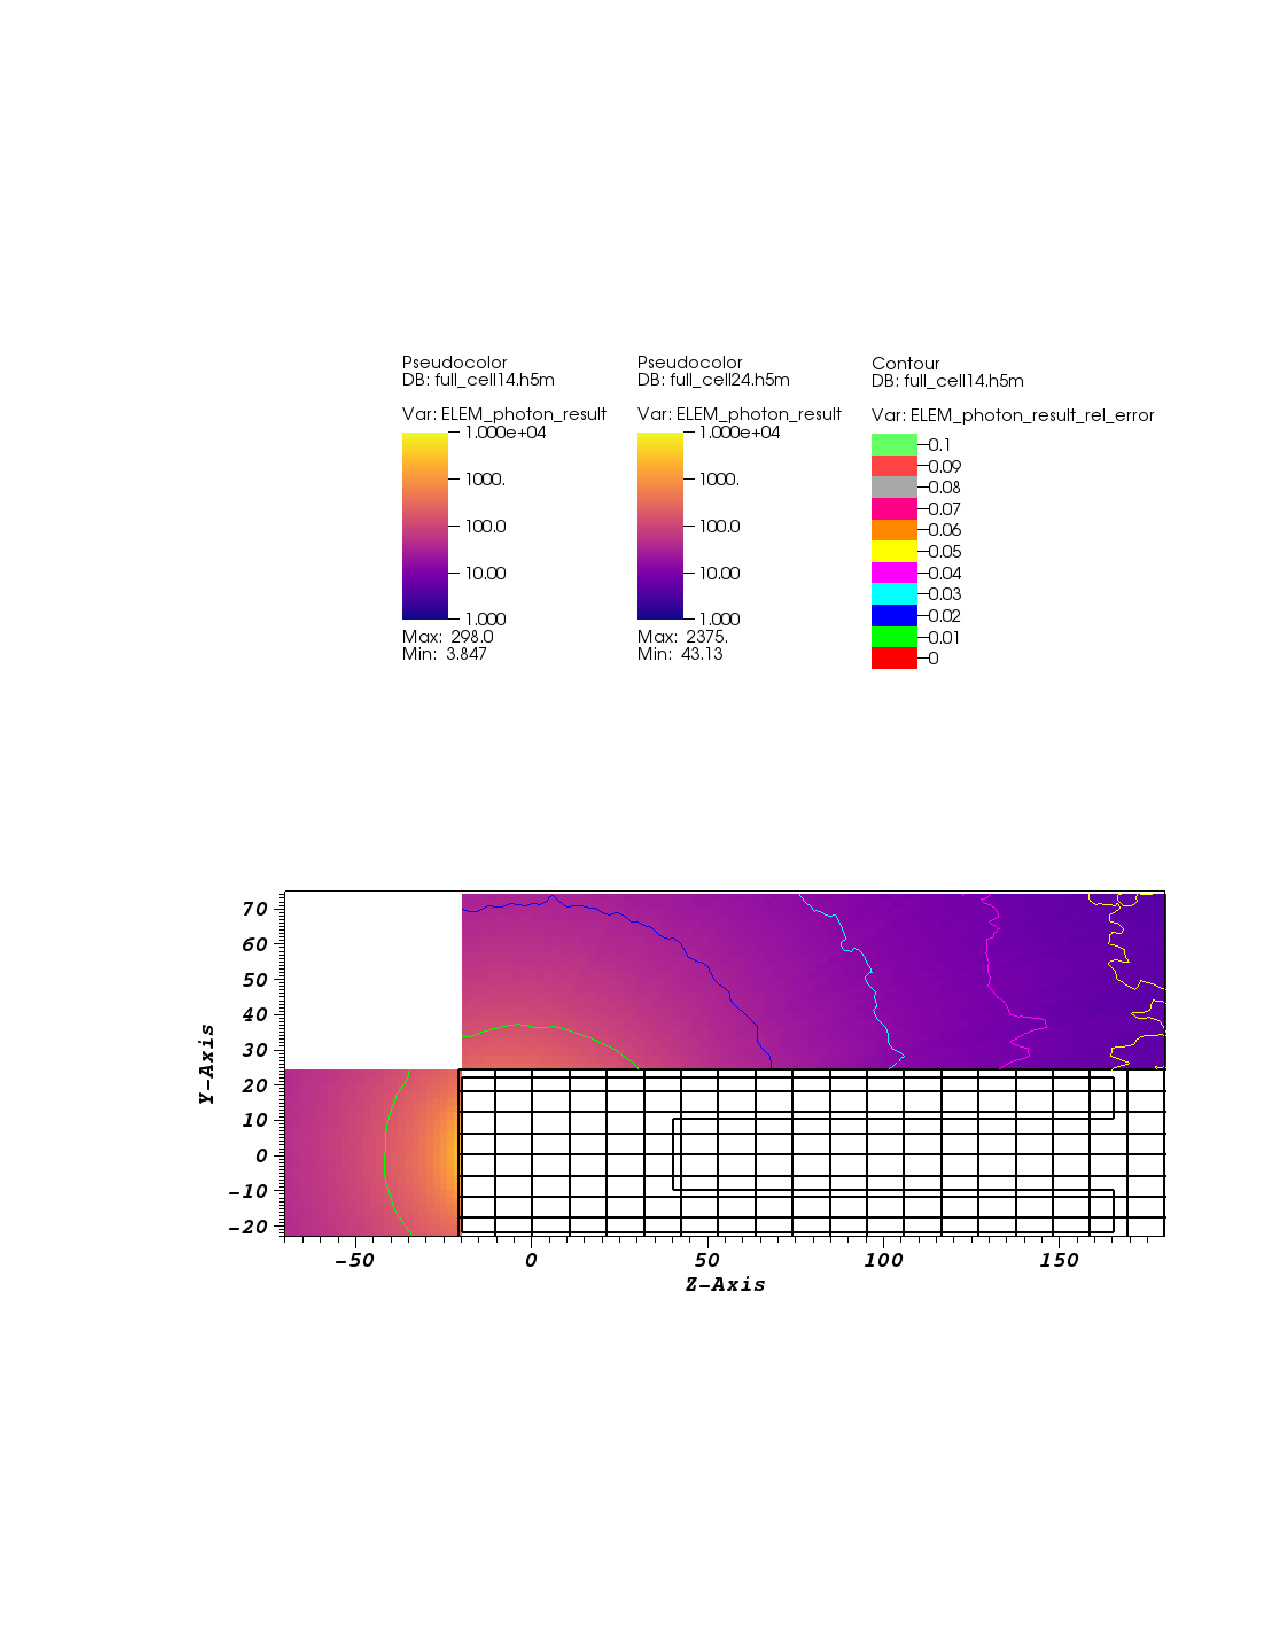
\includegraphics[scale=0.49,trim={20cm 16cm 7cm 5cm},clip]{figs/dose_mer_cell_void.pdf}
        \end{figure}

\end{columns}
\end{frame}

%%%%%%%%%%%%%%%SLIDE %%%%%%
\begin{frame}{Dose Ratio: Mercury Source, Void Steel Volumes}
	\begin{equation}
		ratio = \frac{Mesh}{Cell}
	\end{equation}
\begin{columns}[T]
	\column{0.7\textwidth}

        \begin{figure}
                \centering
		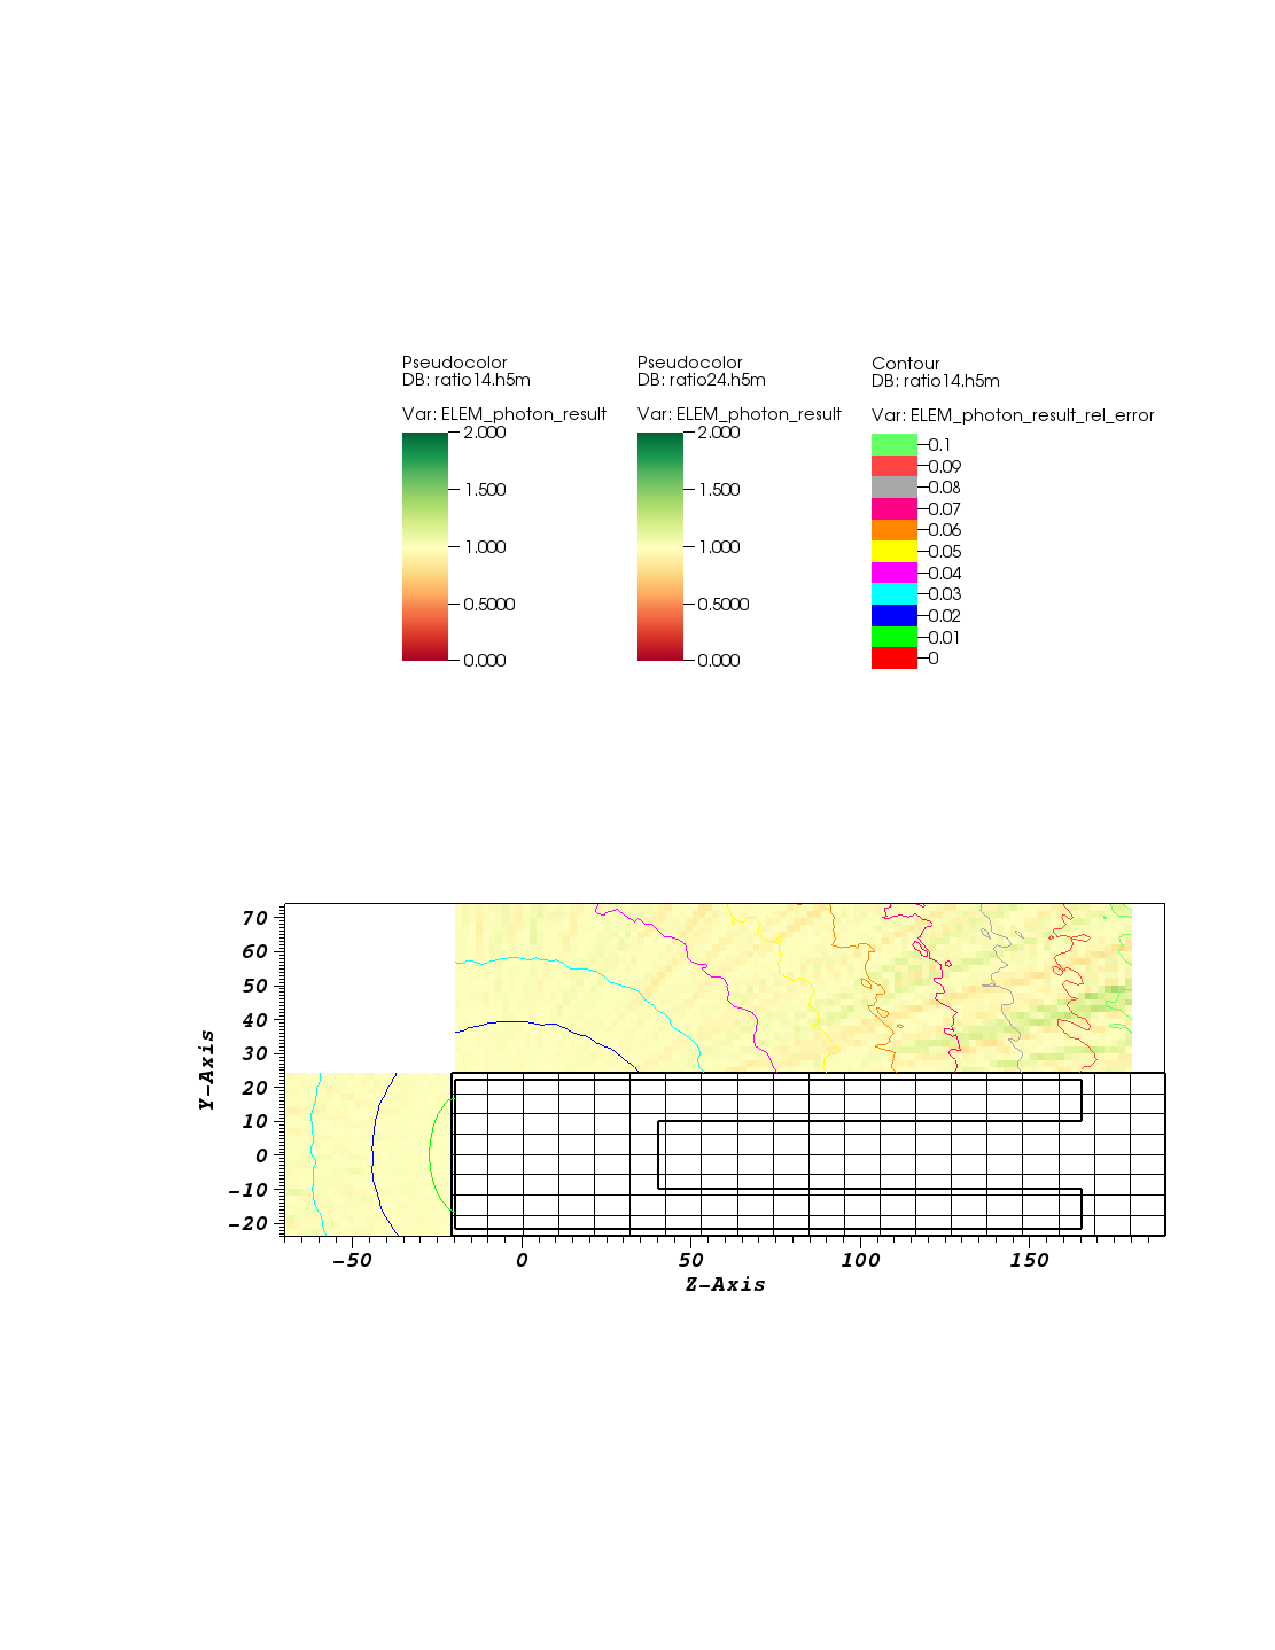
\includegraphics[scale=0.49,trim={2.5cm 6cm 1cm 15cm},clip]{figs/ratio_mer_void.pdf}
        \end{figure}

	\column{0.15\textwidth}
        \begin{figure}
                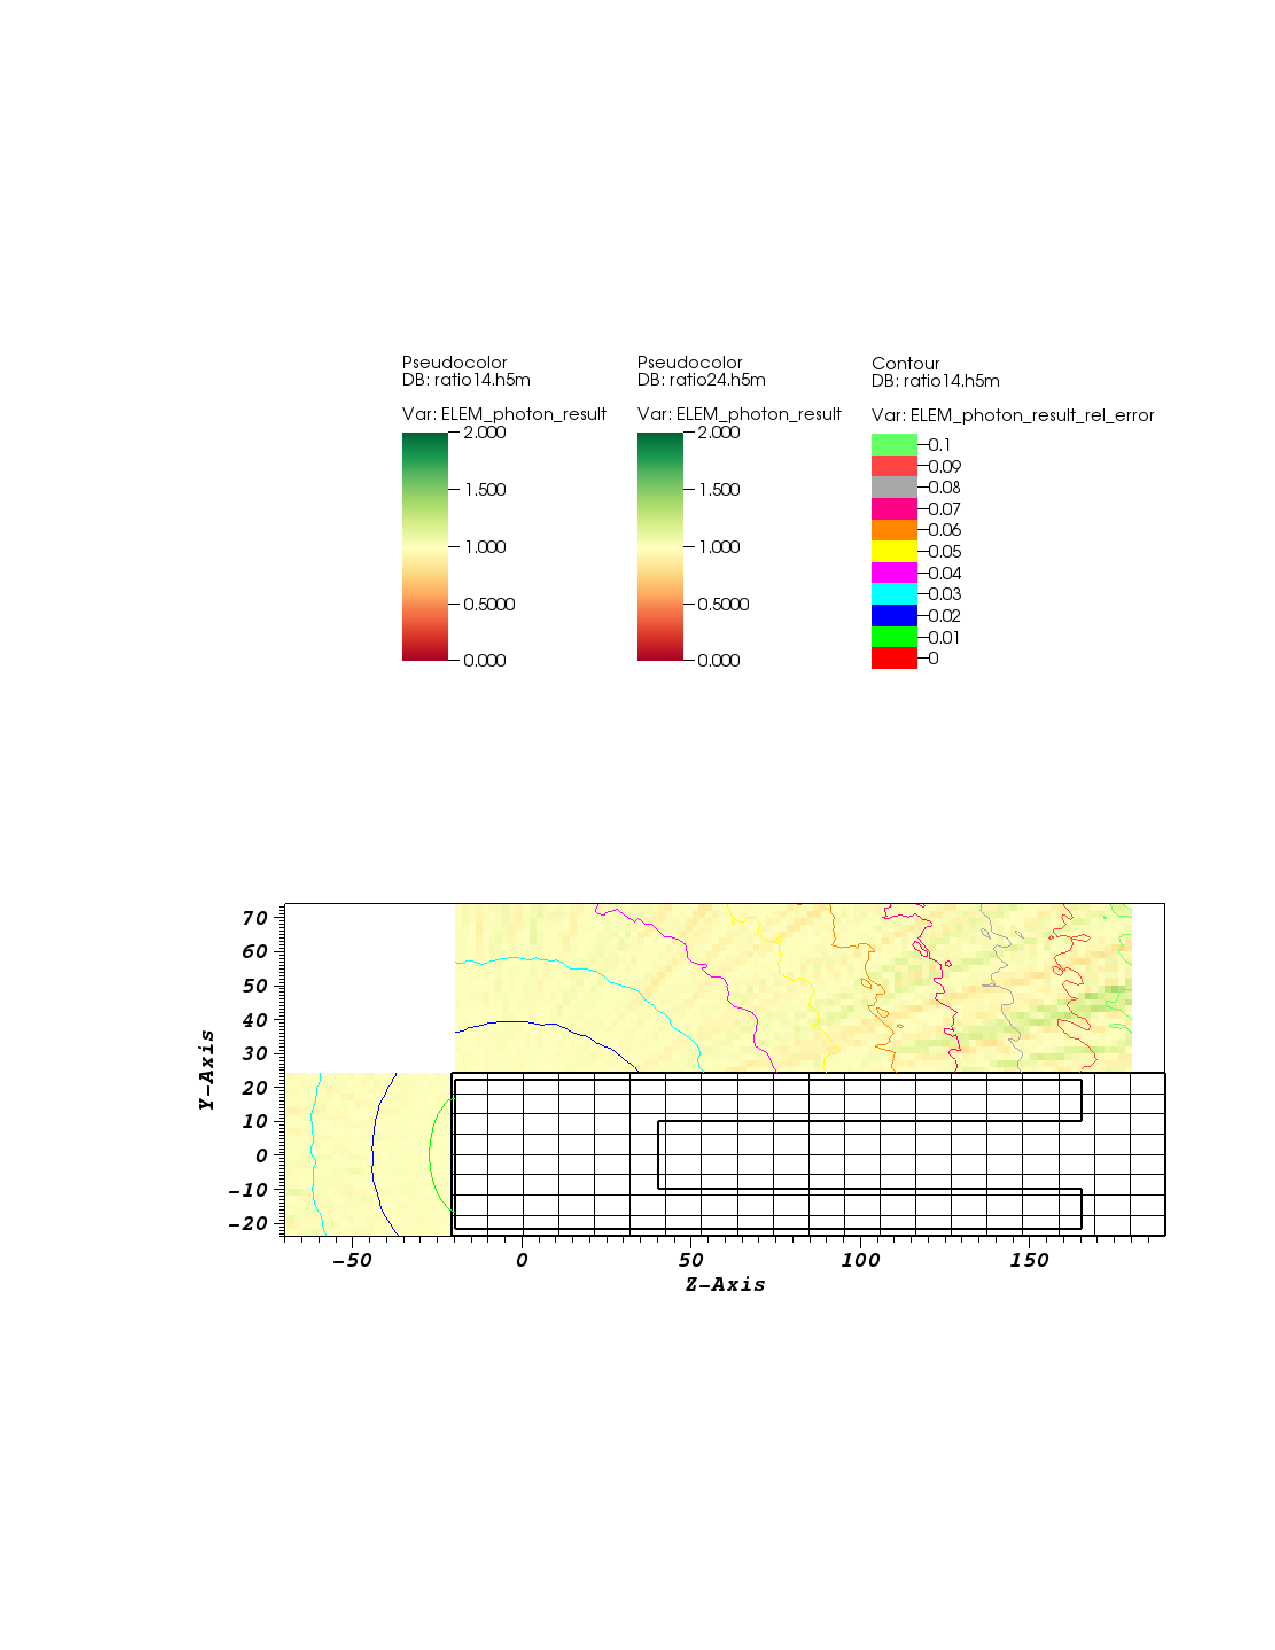
\includegraphics[scale=0.49,trim={6.75cm 16.5cm 11cm 6cm},clip]{figs/ratio_mer_void.pdf}
        \end{figure}
	\column{0.1\textwidth}
        \begin{figure}
                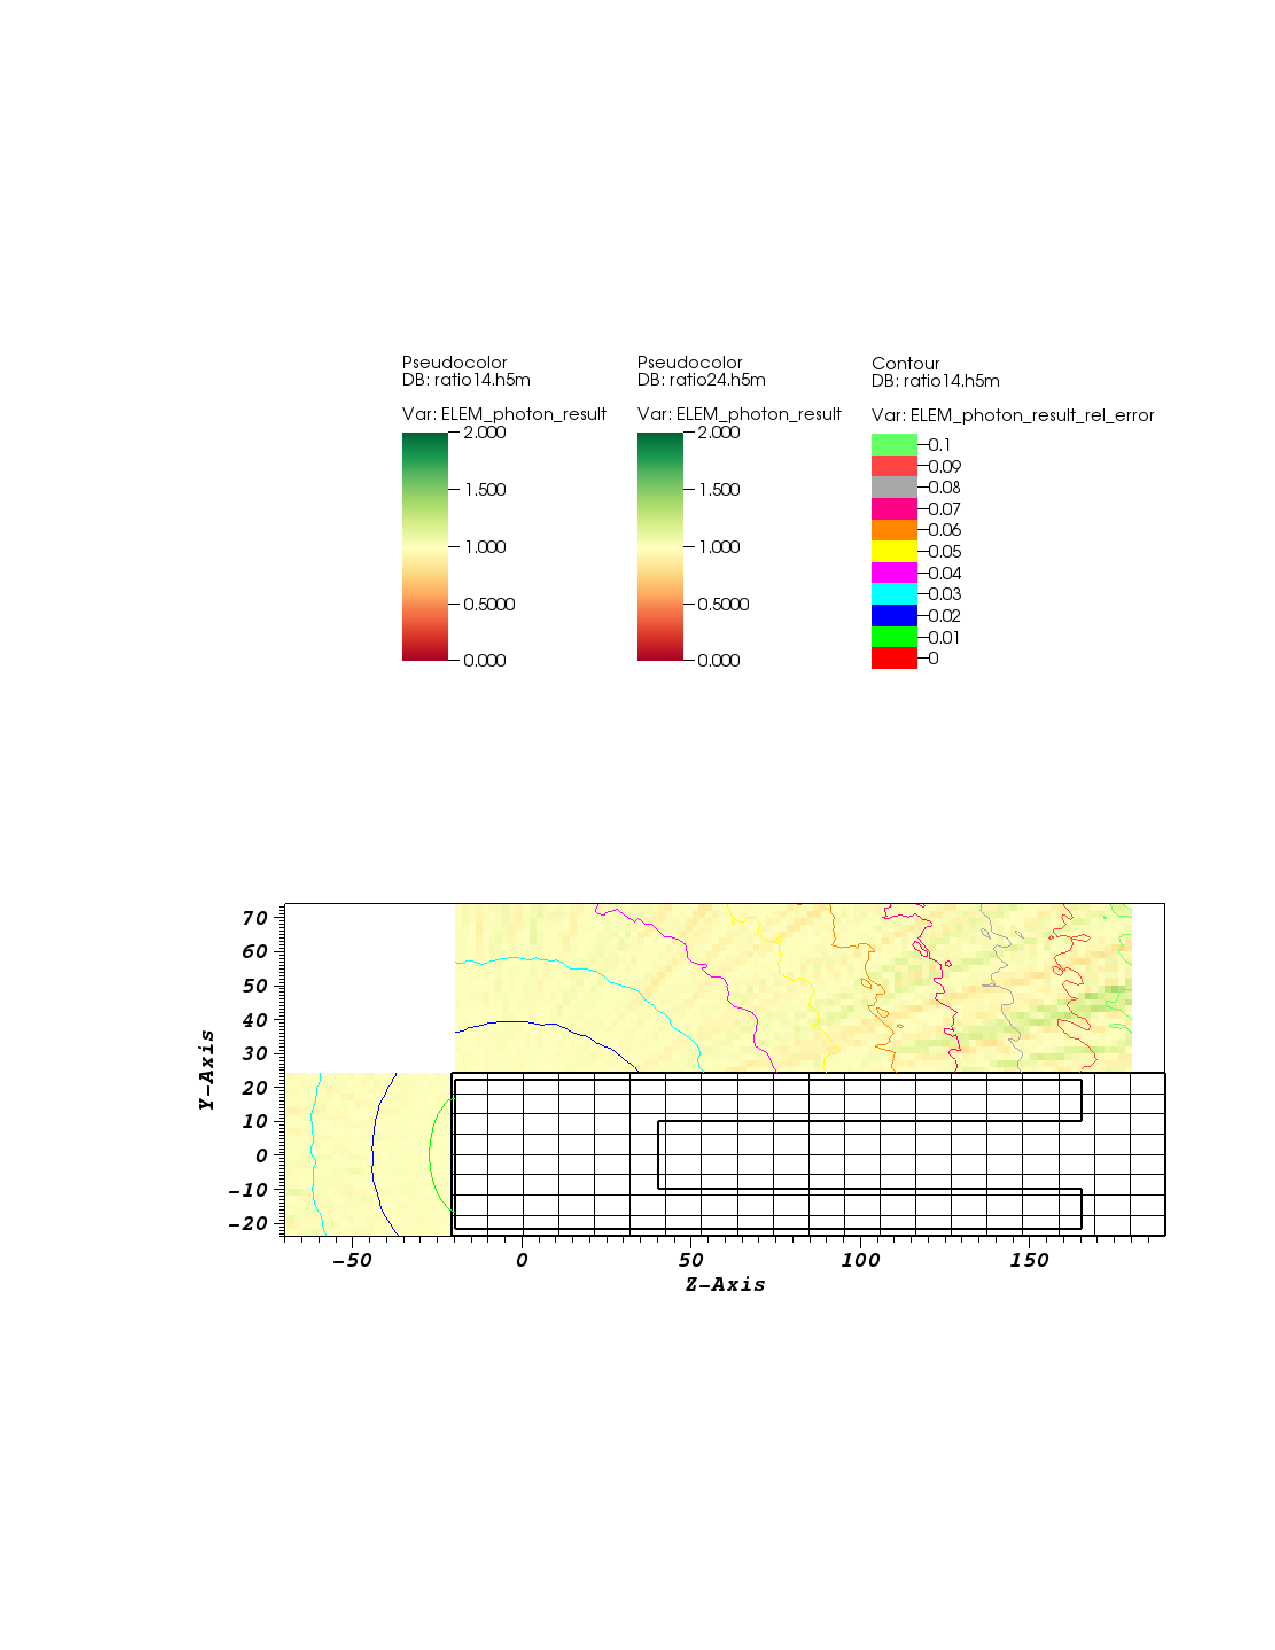
\includegraphics[scale=0.49,trim={20cm 16.5cm 7cm 6cm},clip]{figs/ratio_mer_void.pdf}
        \end{figure}

\end{columns}
\end{frame}

%%%%%%%%%%%%%%%%%%%% SLIDE

\begin{frame}{Dose Rates: Steel Source, Void Mercury Volumes}
\begin{columns}[T]
        \column{0.8\textwidth}
        \textbf{Cell Workflow}
        \begin{figure}
                \centering
                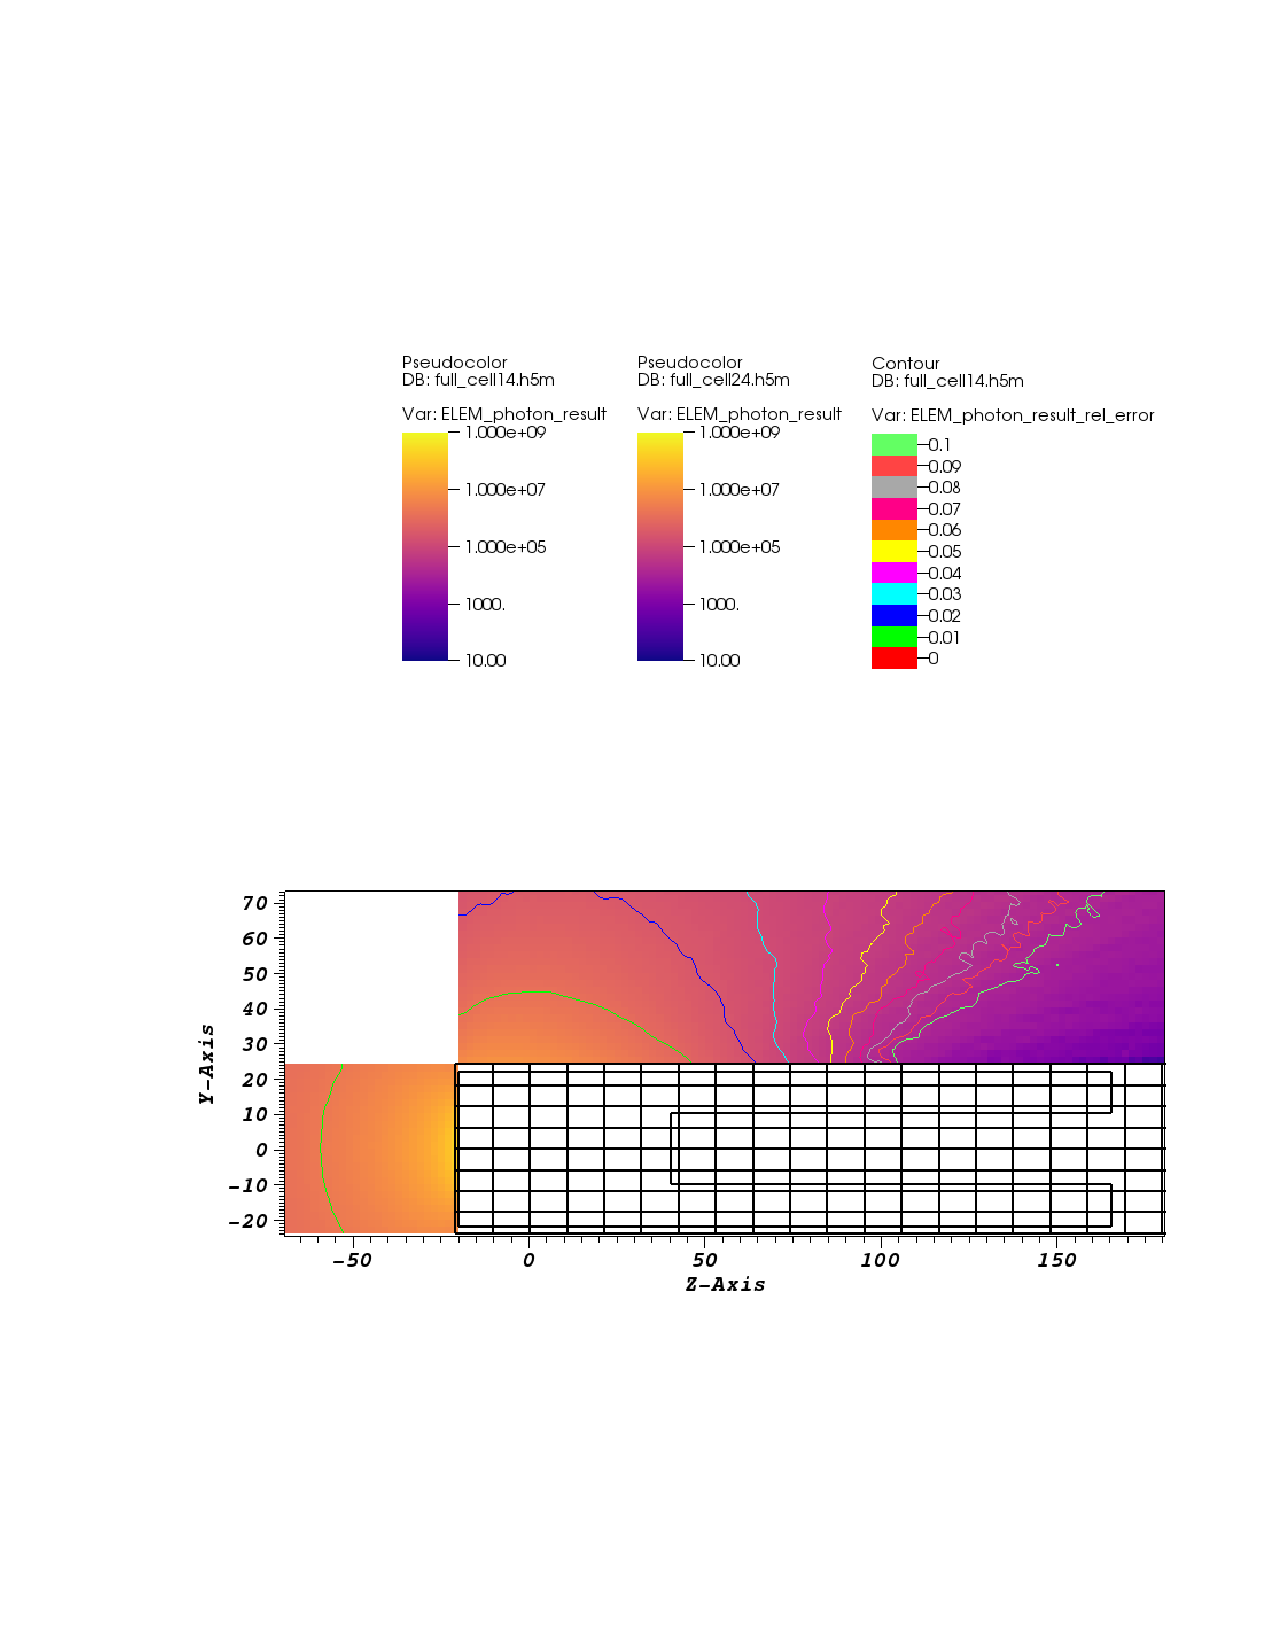
\includegraphics[scale=0.49,trim={2.5cm 6cm 1cm 15cm},clip]{figs/dose_steel_cell_void.pdf}
        \end{figure}

        \column{0.2\textwidth}

	\tiny{* thick line = geom} \\
	\tiny{* thin line = src mesh}

        \begin{figure}
                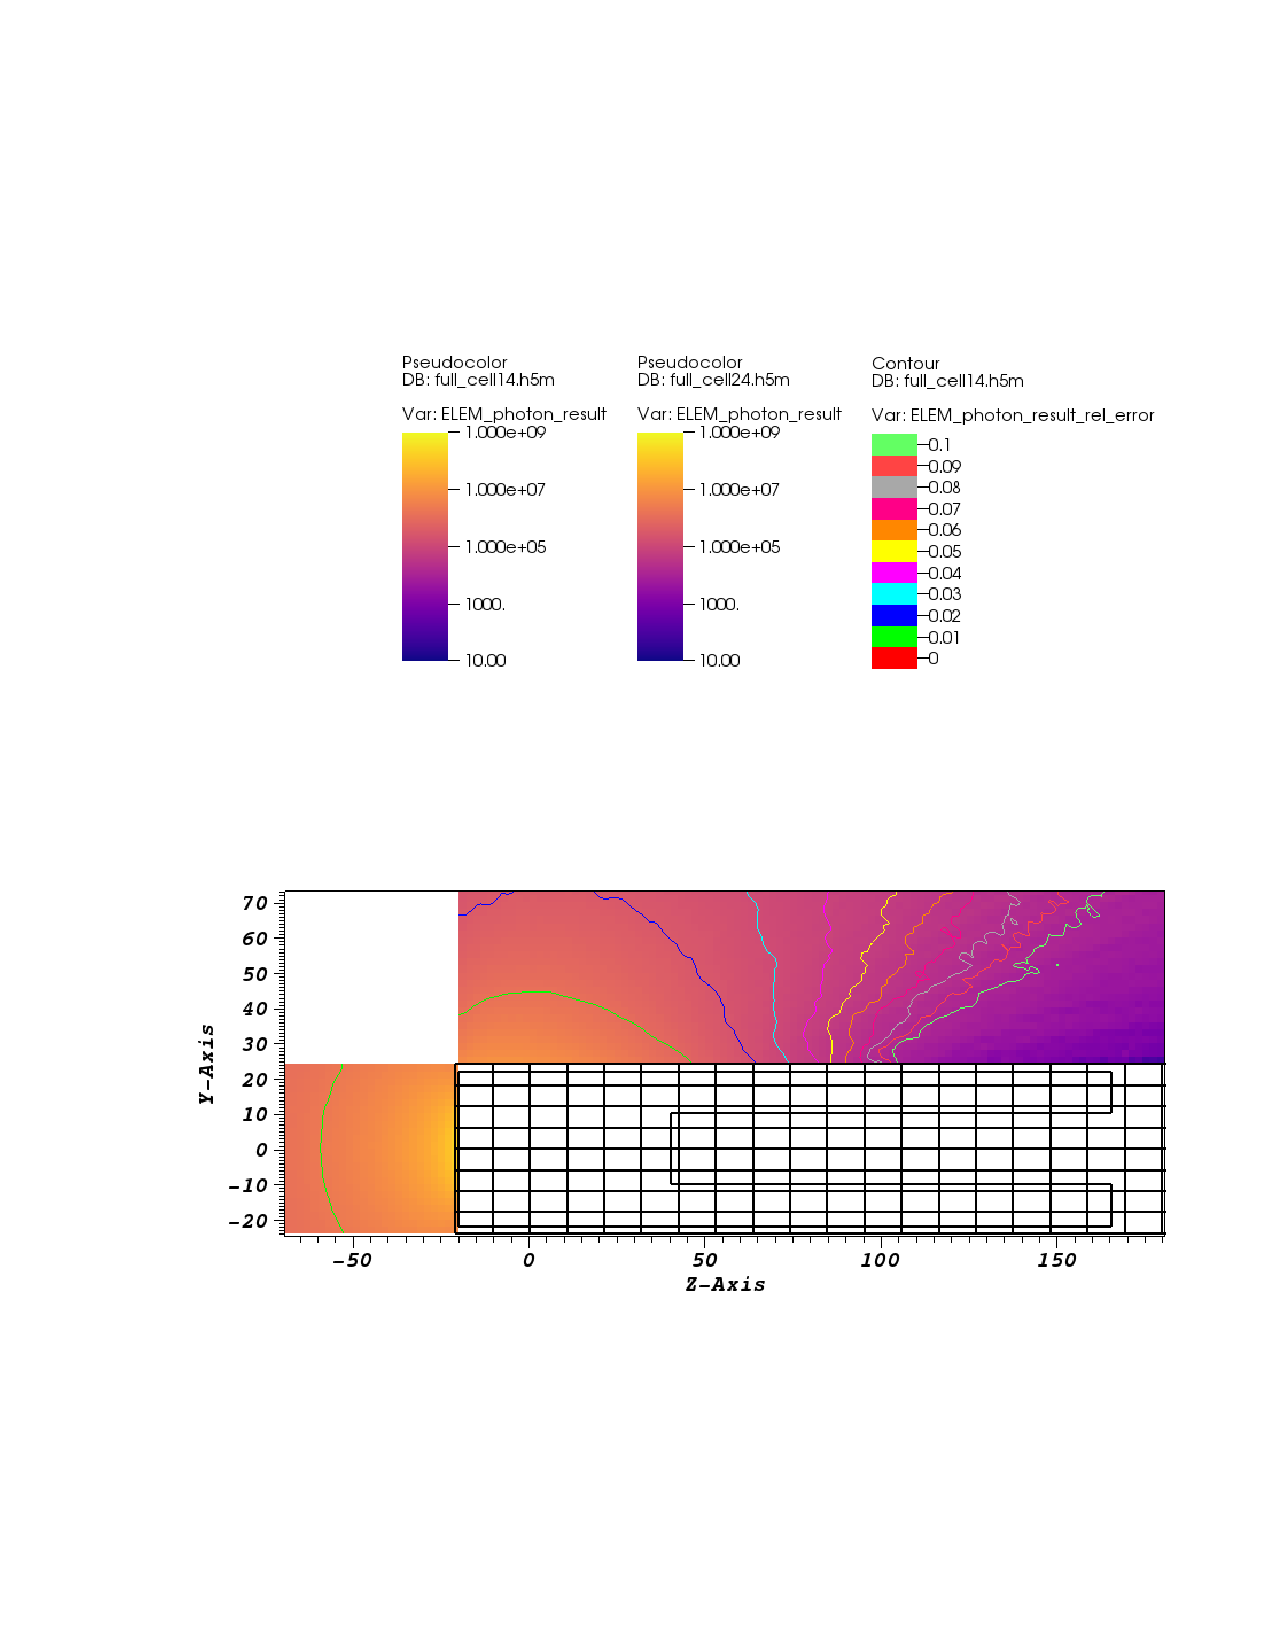
\includegraphics[scale=0.49,trim={6.75cm 16.5cm 11cm 6cm},clip]{figs/dose_steel_cell_void.pdf}
        \end{figure}
\end{columns}

\begin{columns}[T]
        \column{0.8\textwidth}

        \textbf{Mesh Workflow}
        \begin{figure}
                \centering
                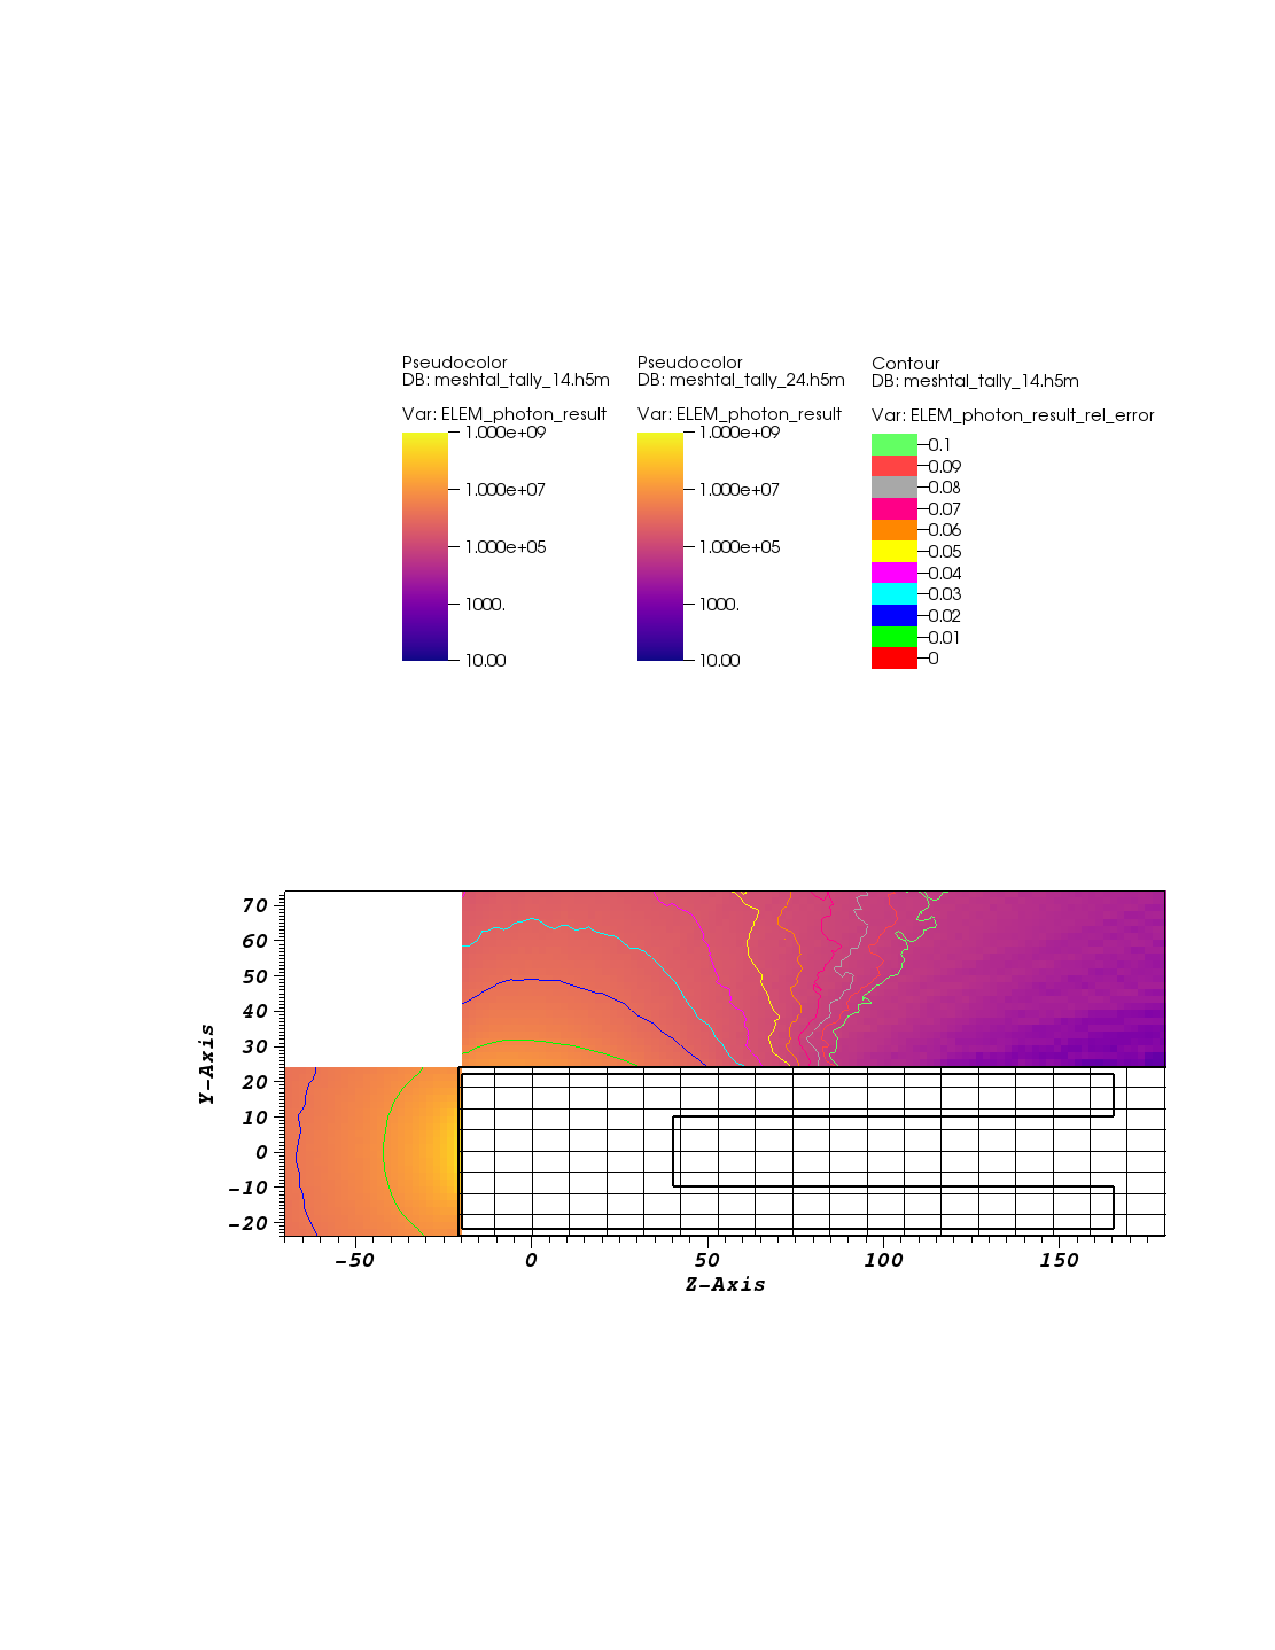
\includegraphics[scale=0.49,trim={2.5cm 6cm 1cm 15cm},clip]{figs/dose_steel_mesh_void.pdf}
        \end{figure}

        \column{0.2\textwidth}
        \begin{figure}
                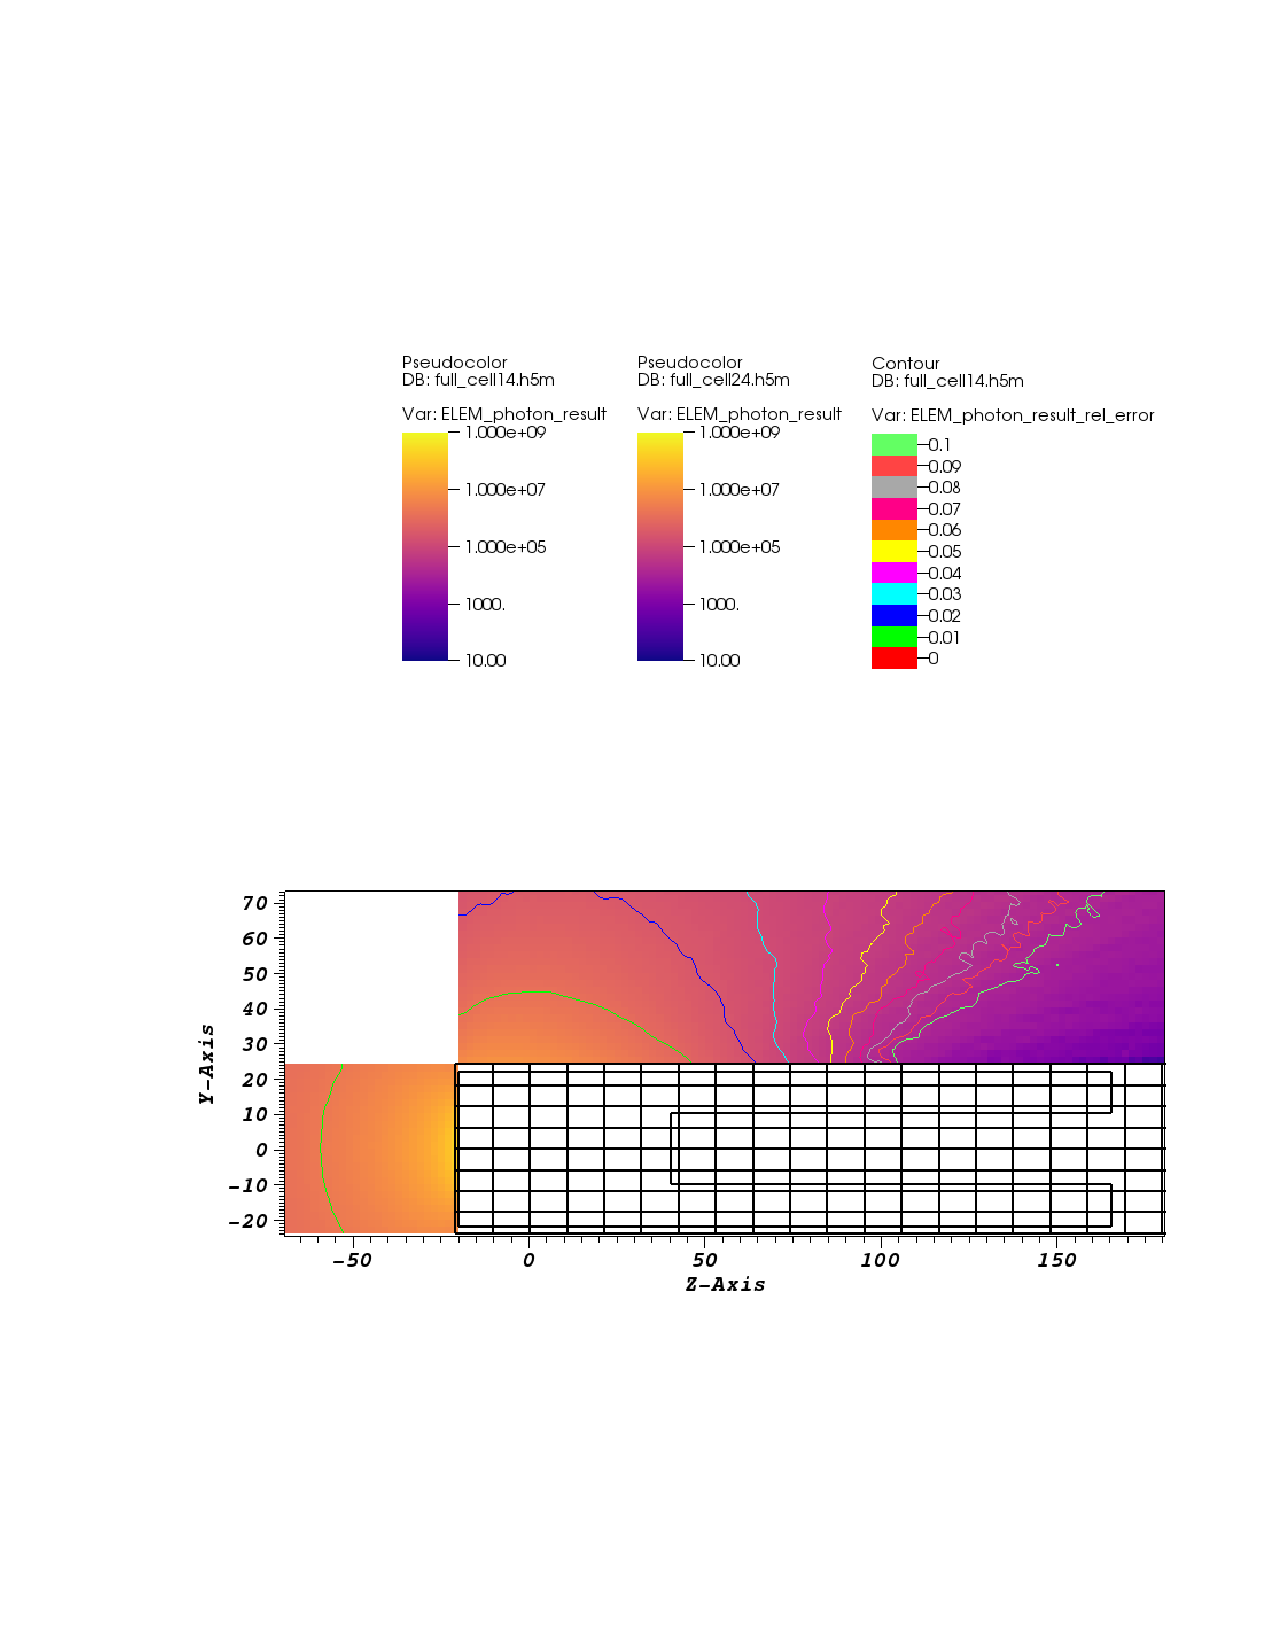
\includegraphics[scale=0.49,trim={20cm 16cm 7cm 5cm},clip]{figs/dose_steel_cell_void.pdf}
        \end{figure}

\end{columns}
\end{frame}

%%%%%%%%%%%%%%%SLIDE %%%%%%
\begin{frame}{Dose Ratio: Steel Source, Void Mercury Volumes}
\begin{columns}[T]
	\column{0.7\textwidth}

        \begin{figure}
                \centering
                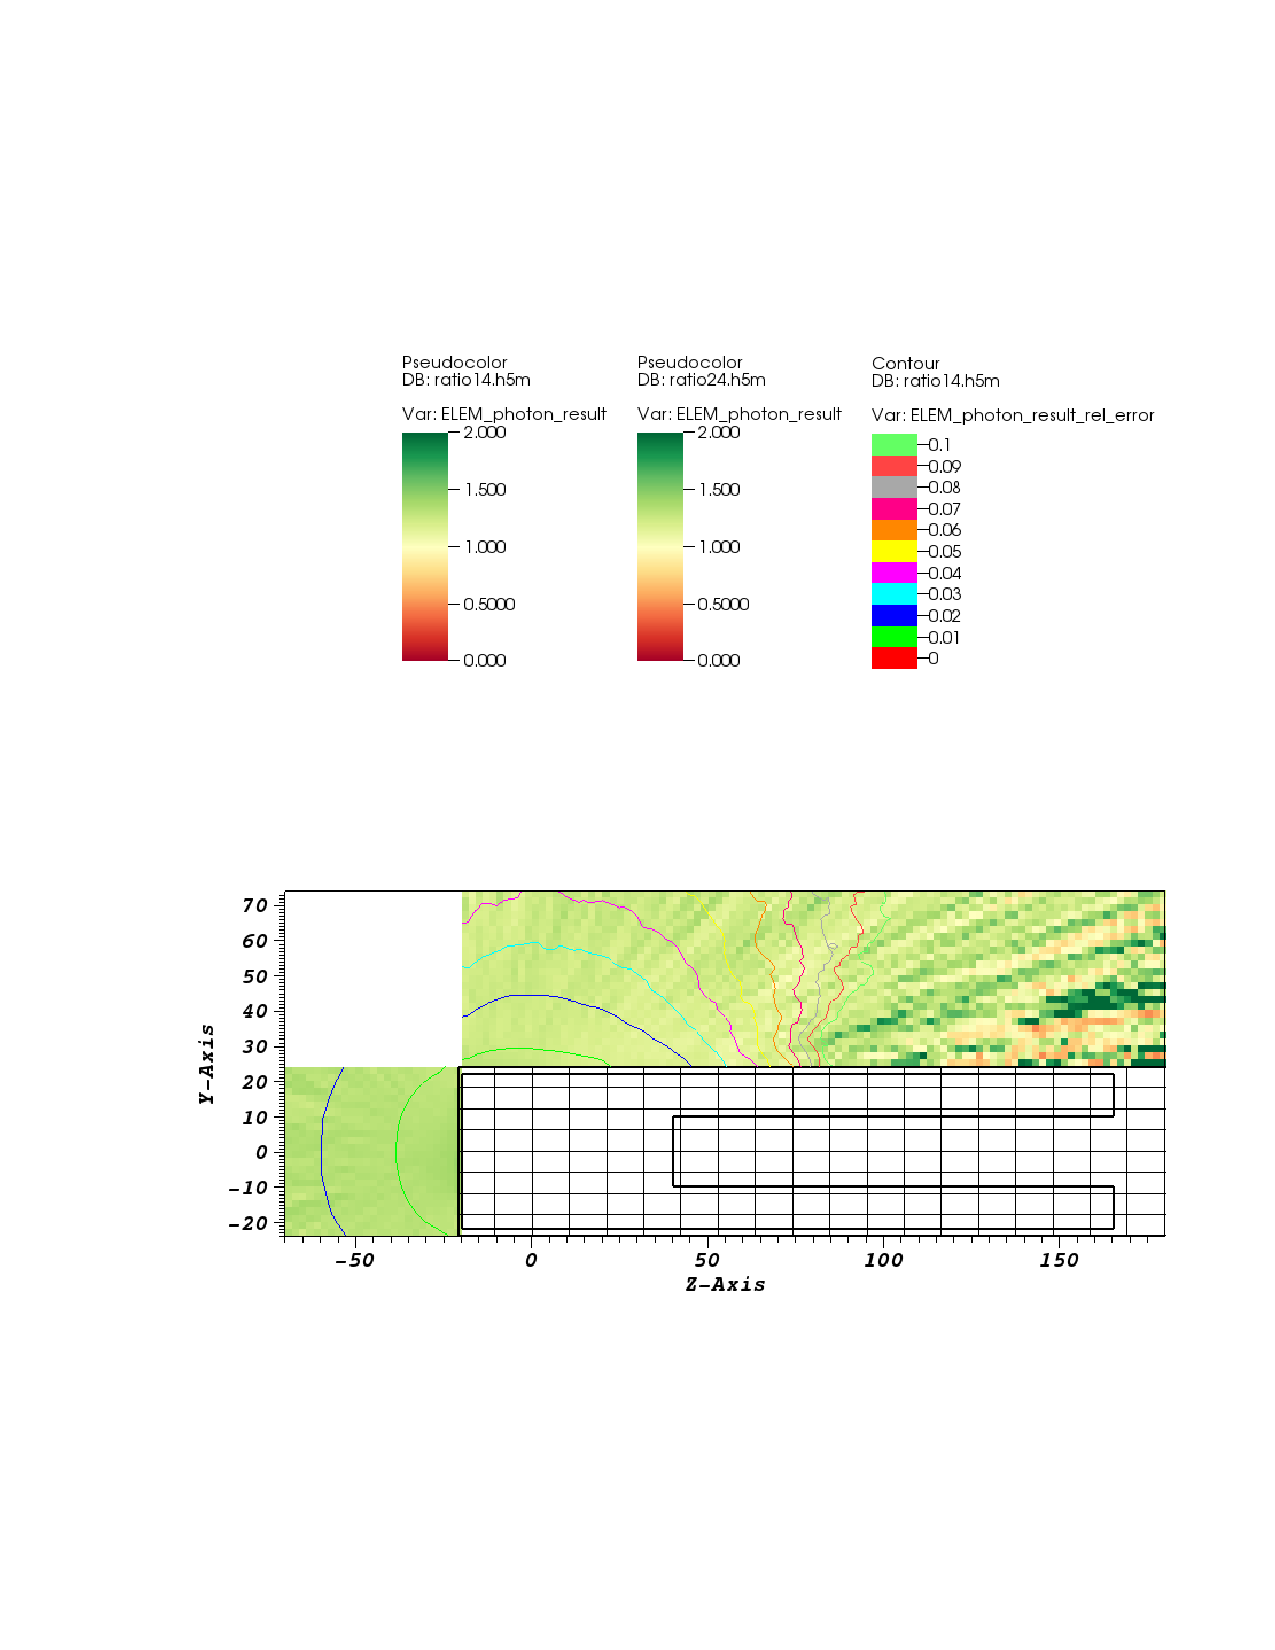
\includegraphics[scale=0.49,trim={2.5cm 6cm 1cm 15cm},clip]{figs/ratio_steel_void.pdf}
        \end{figure}

	\column{0.15\textwidth}
        \begin{figure}
                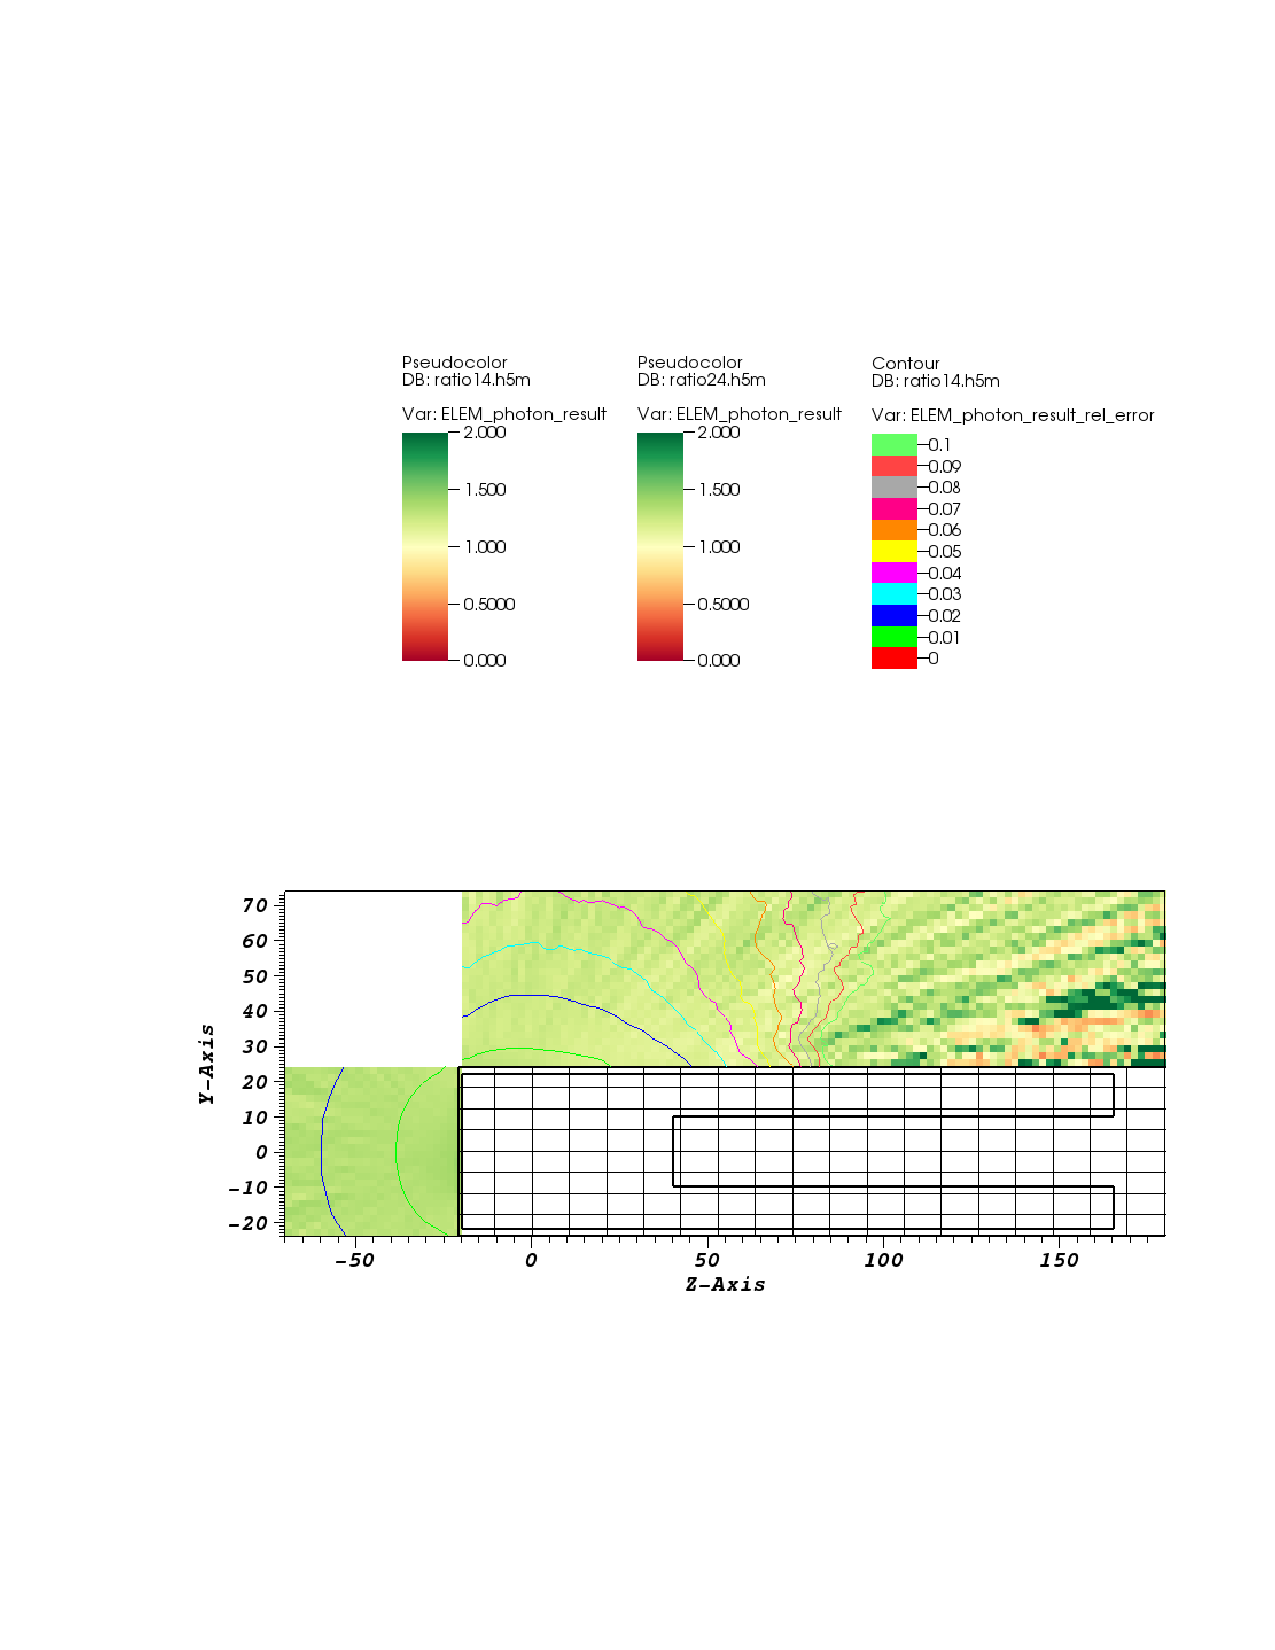
\includegraphics[scale=0.49,trim={6.75cm 16.5cm 11cm 6cm},clip]{figs/ratio_steel_void.pdf}
        \end{figure}
	\column{0.1\textwidth}
        \begin{figure}
                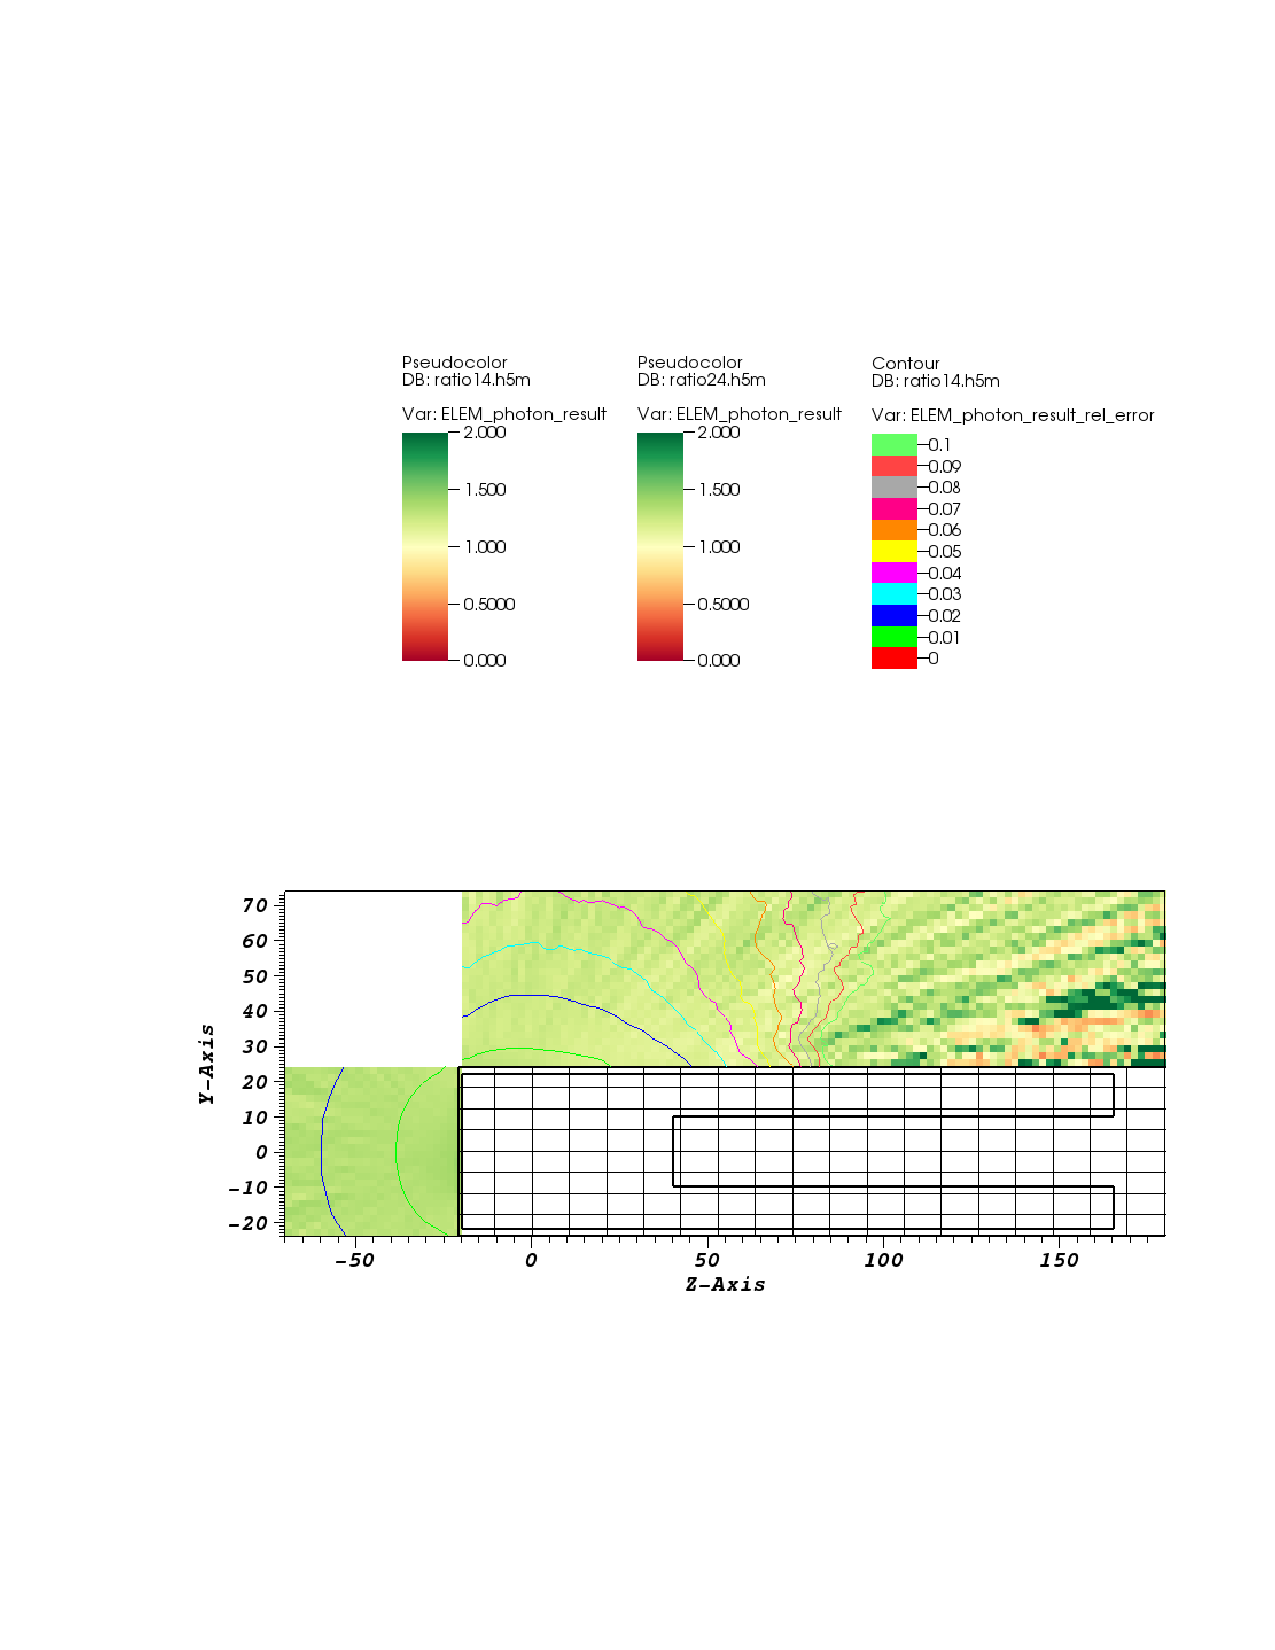
\includegraphics[scale=0.49,trim={20cm 16.5cm 7cm 6cm},clip]{figs/ratio_steel_void.pdf}
        \end{figure}

\end{columns}
\end{frame}

\section{Dose Rates - Full Geometry}

\begin{frame}{Dose Rates: Mercury Source}
\begin{columns}[T]
        \column{0.8\textwidth}
        \textbf{Cell Workflow}
        \begin{figure}
                \centering
                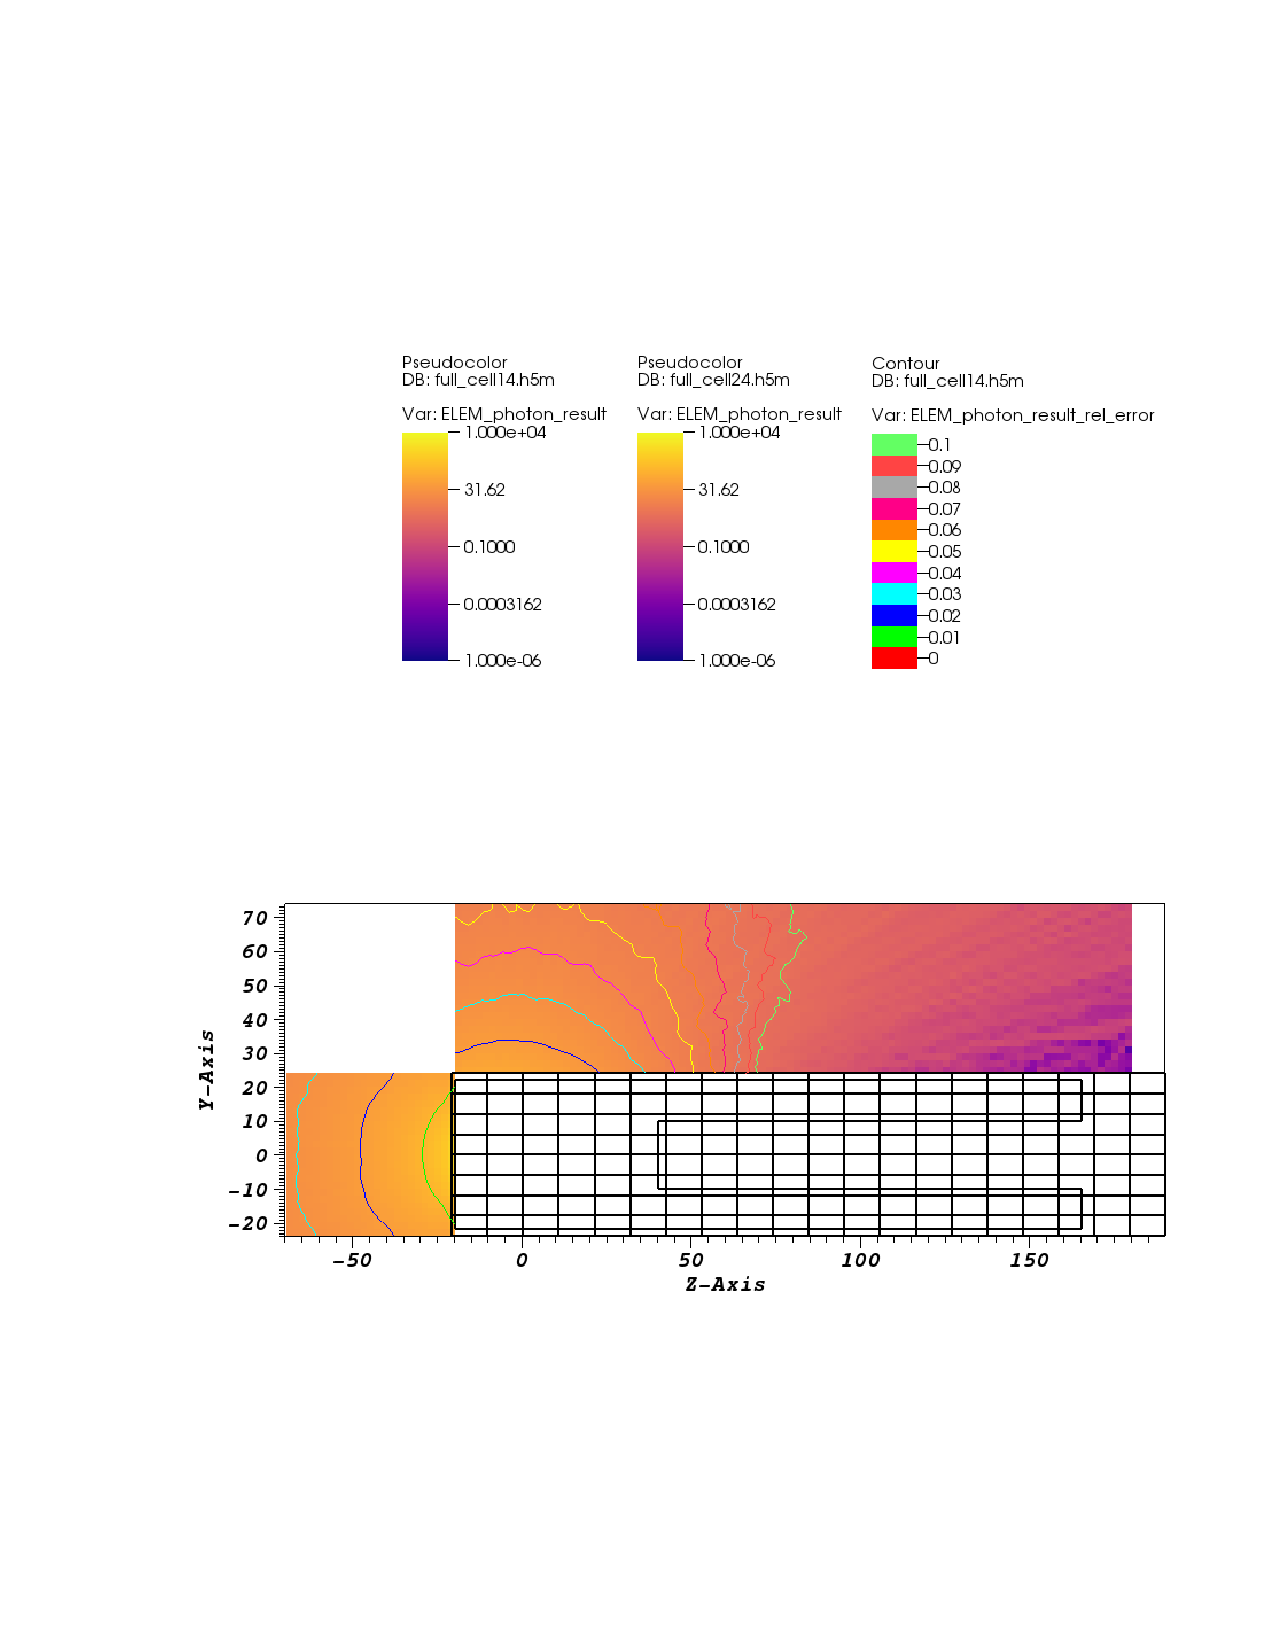
\includegraphics[scale=0.49,trim={2.5cm 6cm 1cm 15cm},clip]{figs/dose_mer_cell_novoid.pdf}
        \end{figure}

        \column{0.2\textwidth}

	\tiny{* thick line = geom} \\
	\tiny{* thin line = src mesh}

        \begin{figure}
                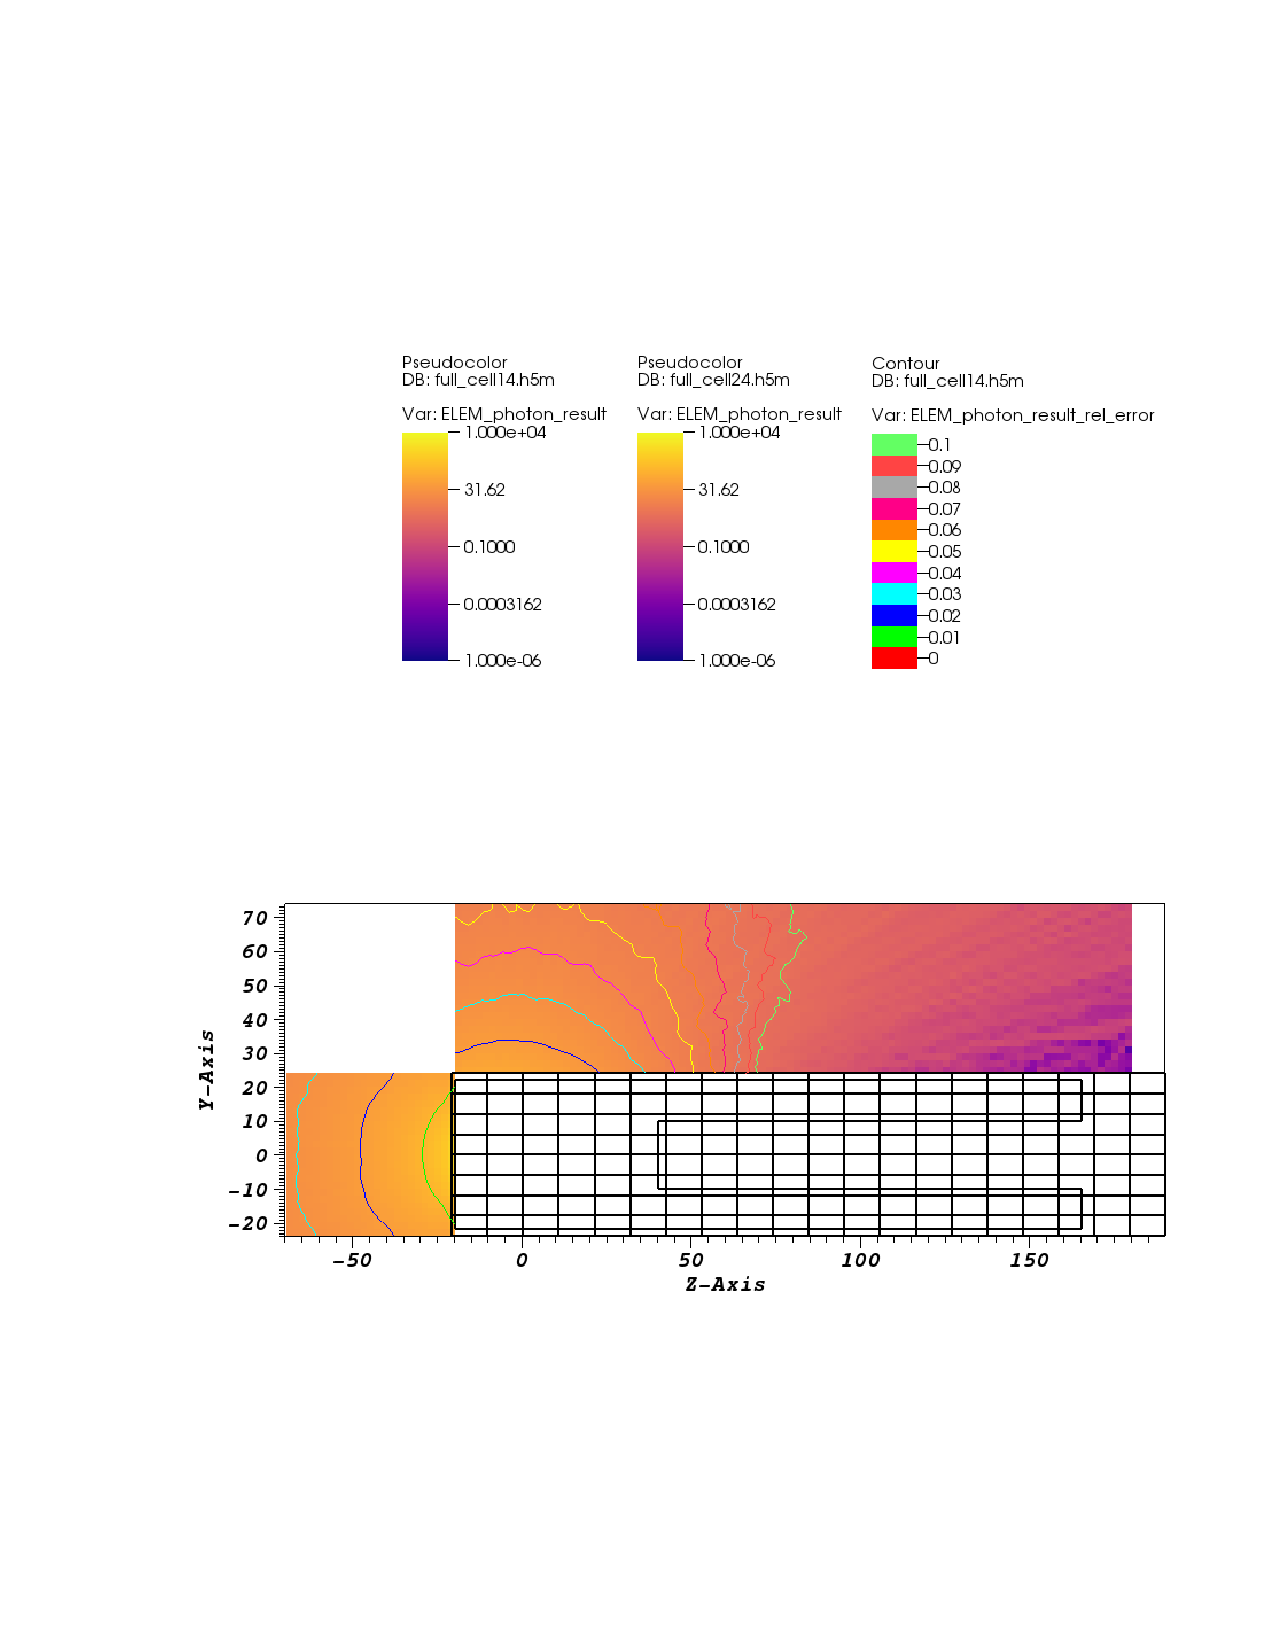
\includegraphics[scale=0.49,trim={6.75cm 16.5cm 11cm 6cm},clip]{figs/dose_mer_cell_novoid.pdf}
        \end{figure}
\end{columns}

\begin{columns}[T]
        \column{0.8\textwidth}

        \textbf{Mesh Workflow}
        \begin{figure}
                \centering
                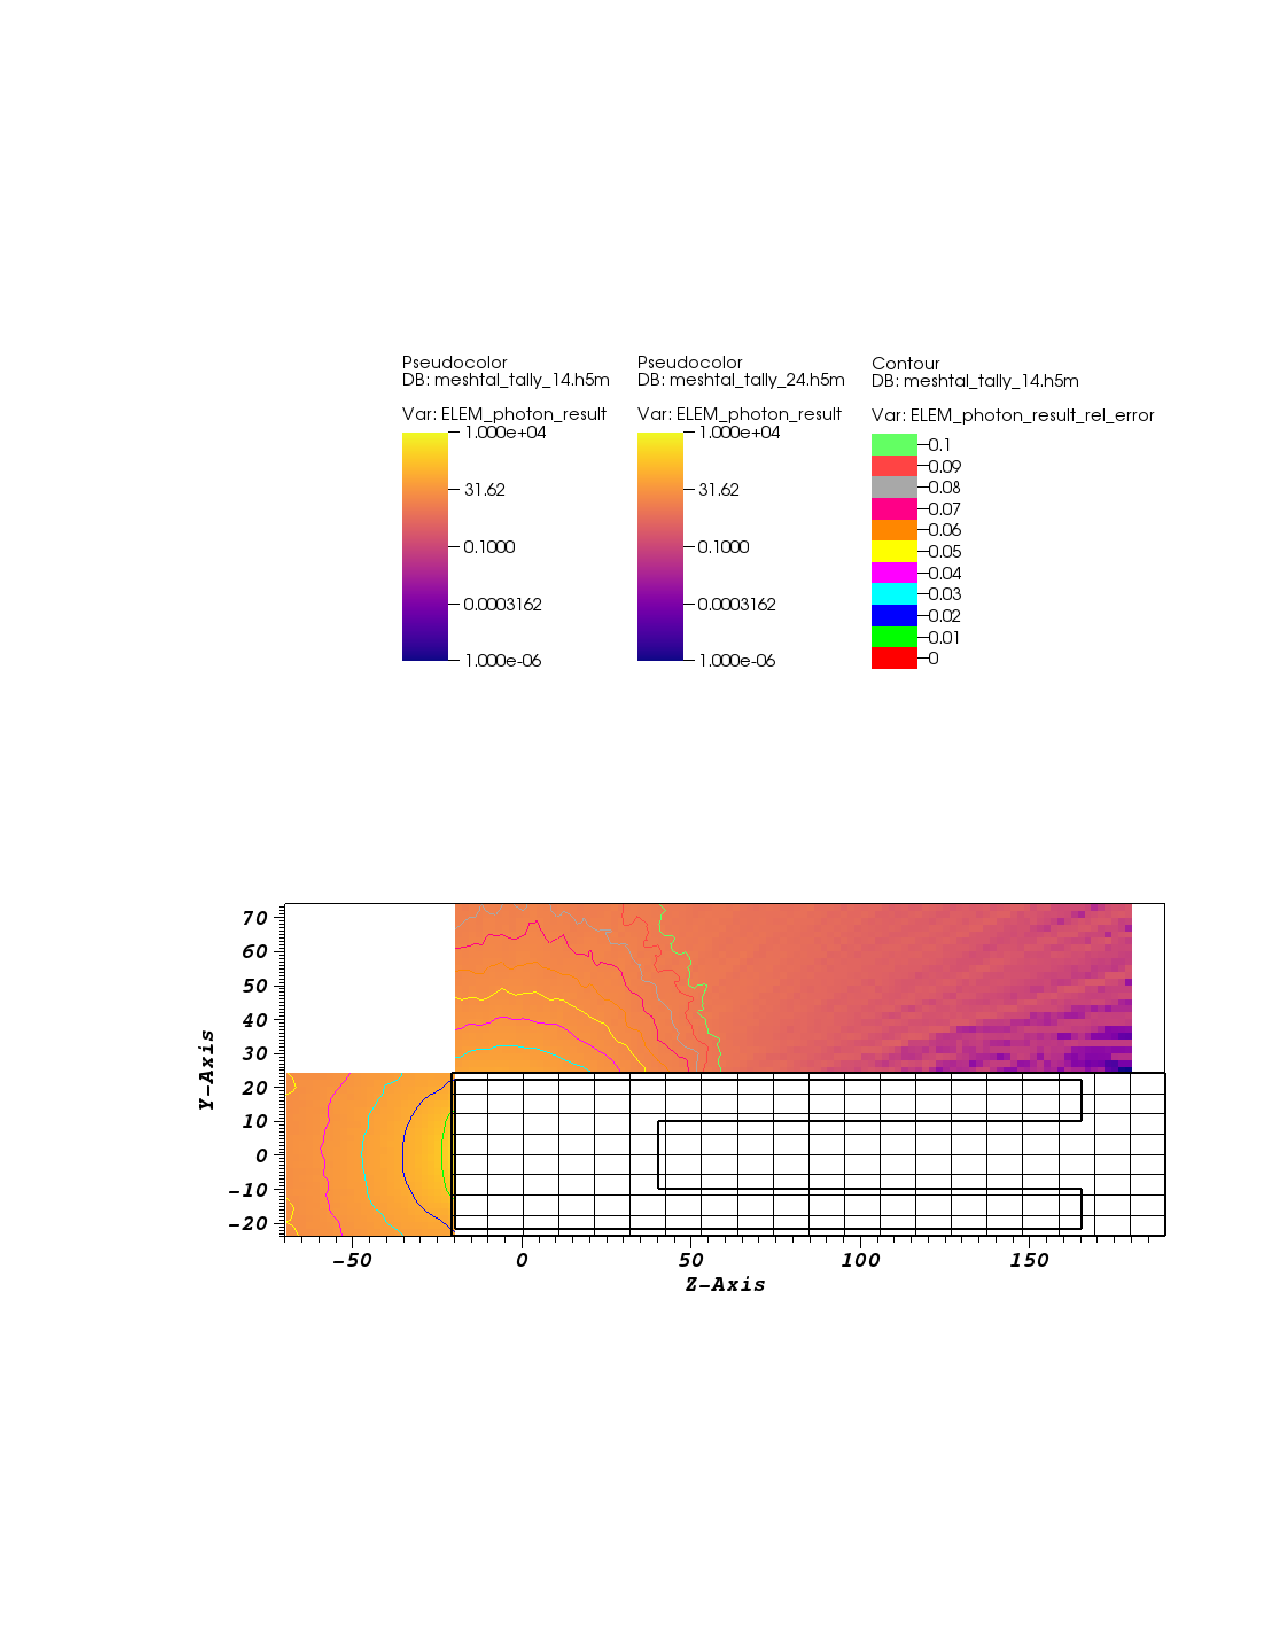
\includegraphics[scale=0.49,trim={2.5cm 6cm 1cm 15cm},clip]{figs/dose_mer_mesh_novoid.pdf}
        \end{figure}

        \column{0.2\textwidth}
        \begin{figure}
                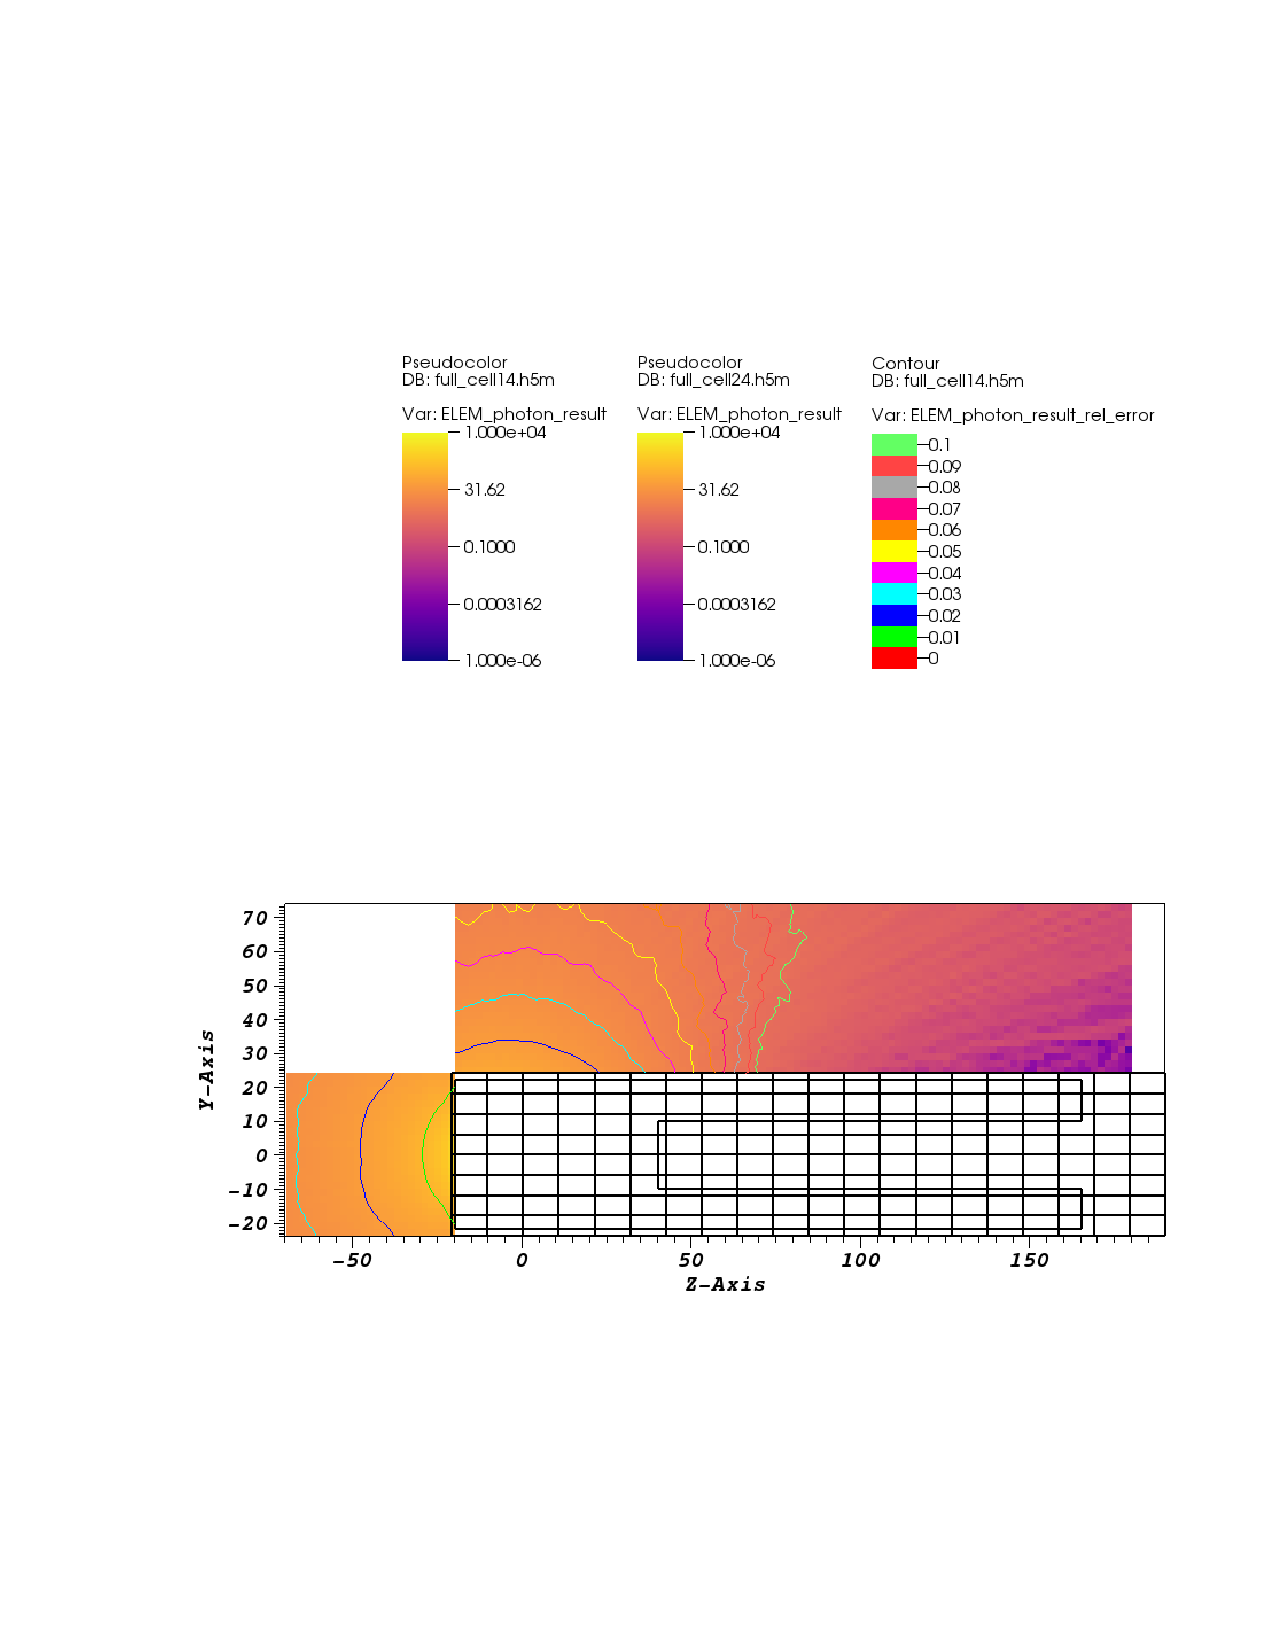
\includegraphics[scale=0.49,trim={20cm 16cm 7cm 5cm},clip]{figs/dose_mer_cell_novoid.pdf}
        \end{figure}

\end{columns}
\end{frame}

%%%%%%%%%%%%%%%SLIDE %%%%%%
\begin{frame}{Dose Ratio: Mercury Source}
\begin{columns}[T]
	\column{0.7\textwidth}

        \begin{figure}
                \centering
                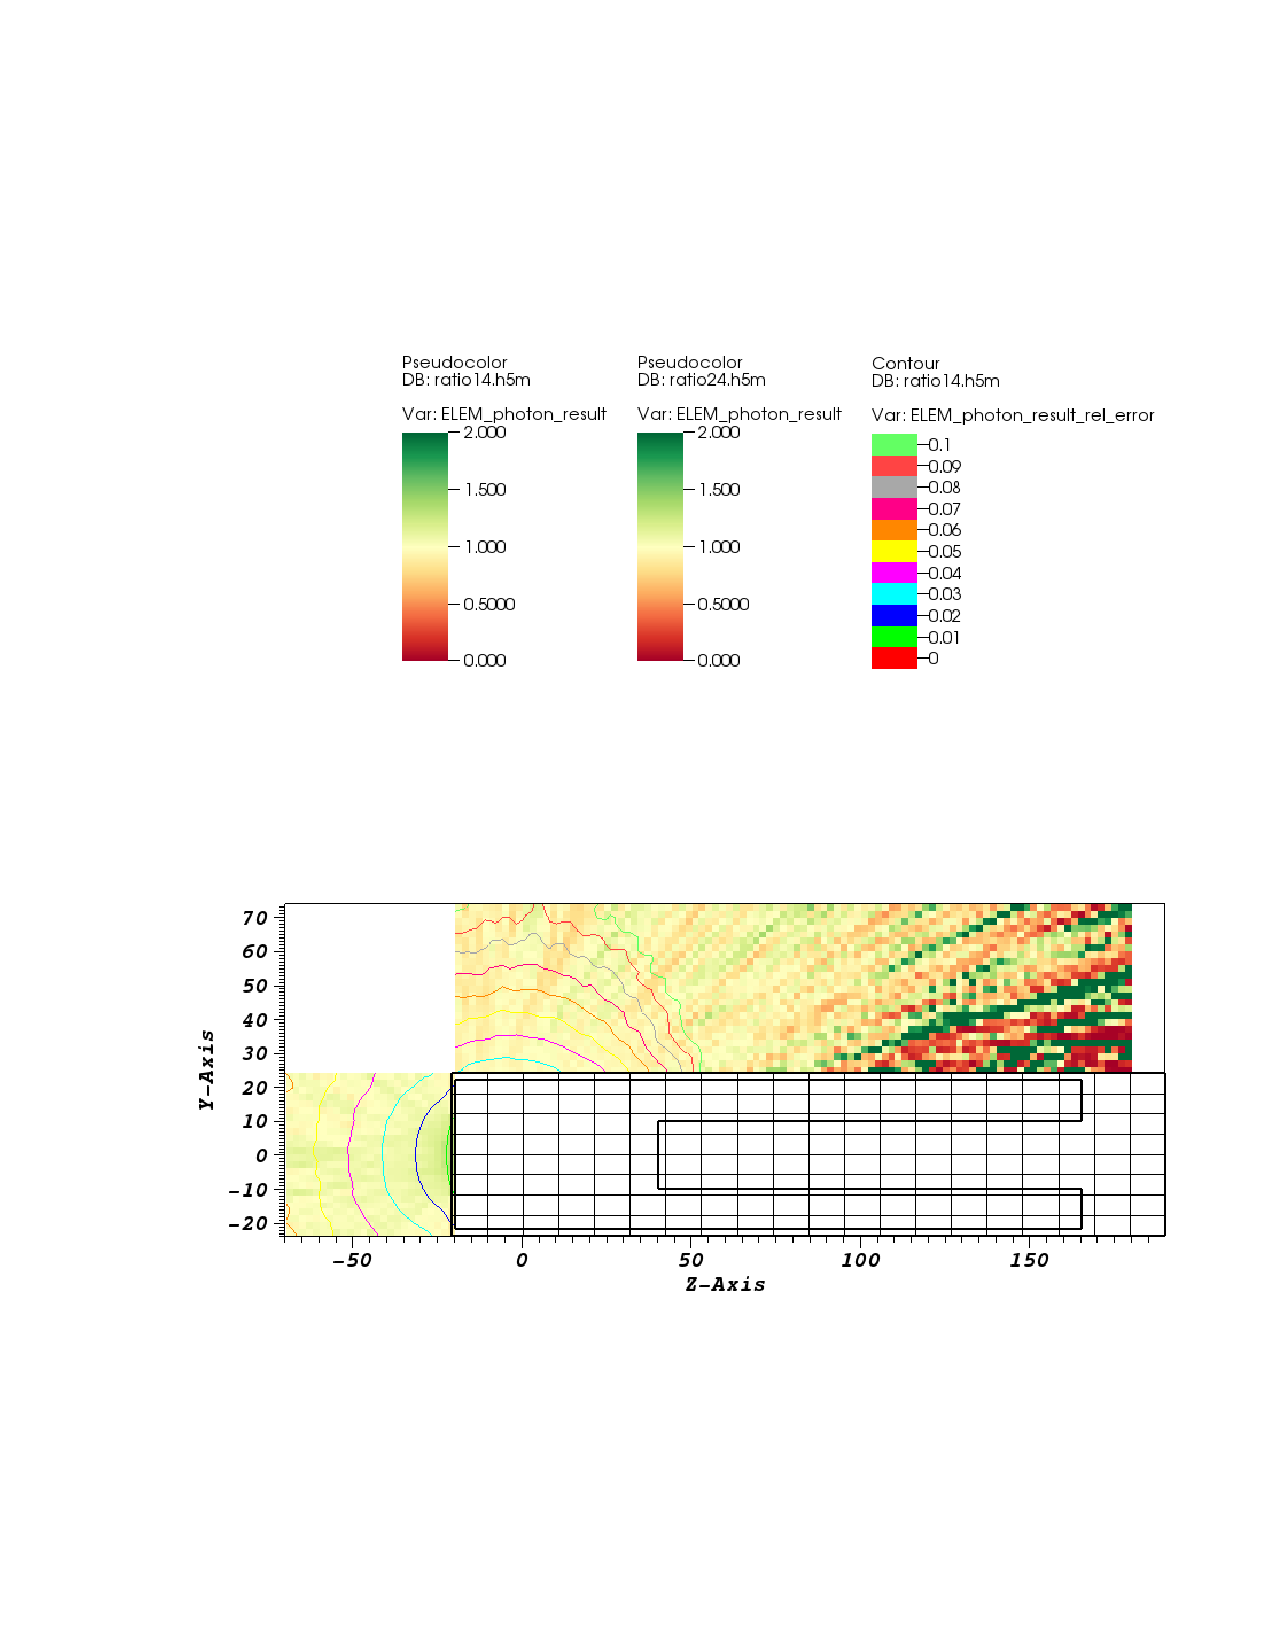
\includegraphics[scale=0.49,trim={2.5cm 6cm 1cm 15cm},clip]{figs/ratio_mer_novoid.pdf}
        \end{figure}

	\column{0.15\textwidth}
        \begin{figure}
                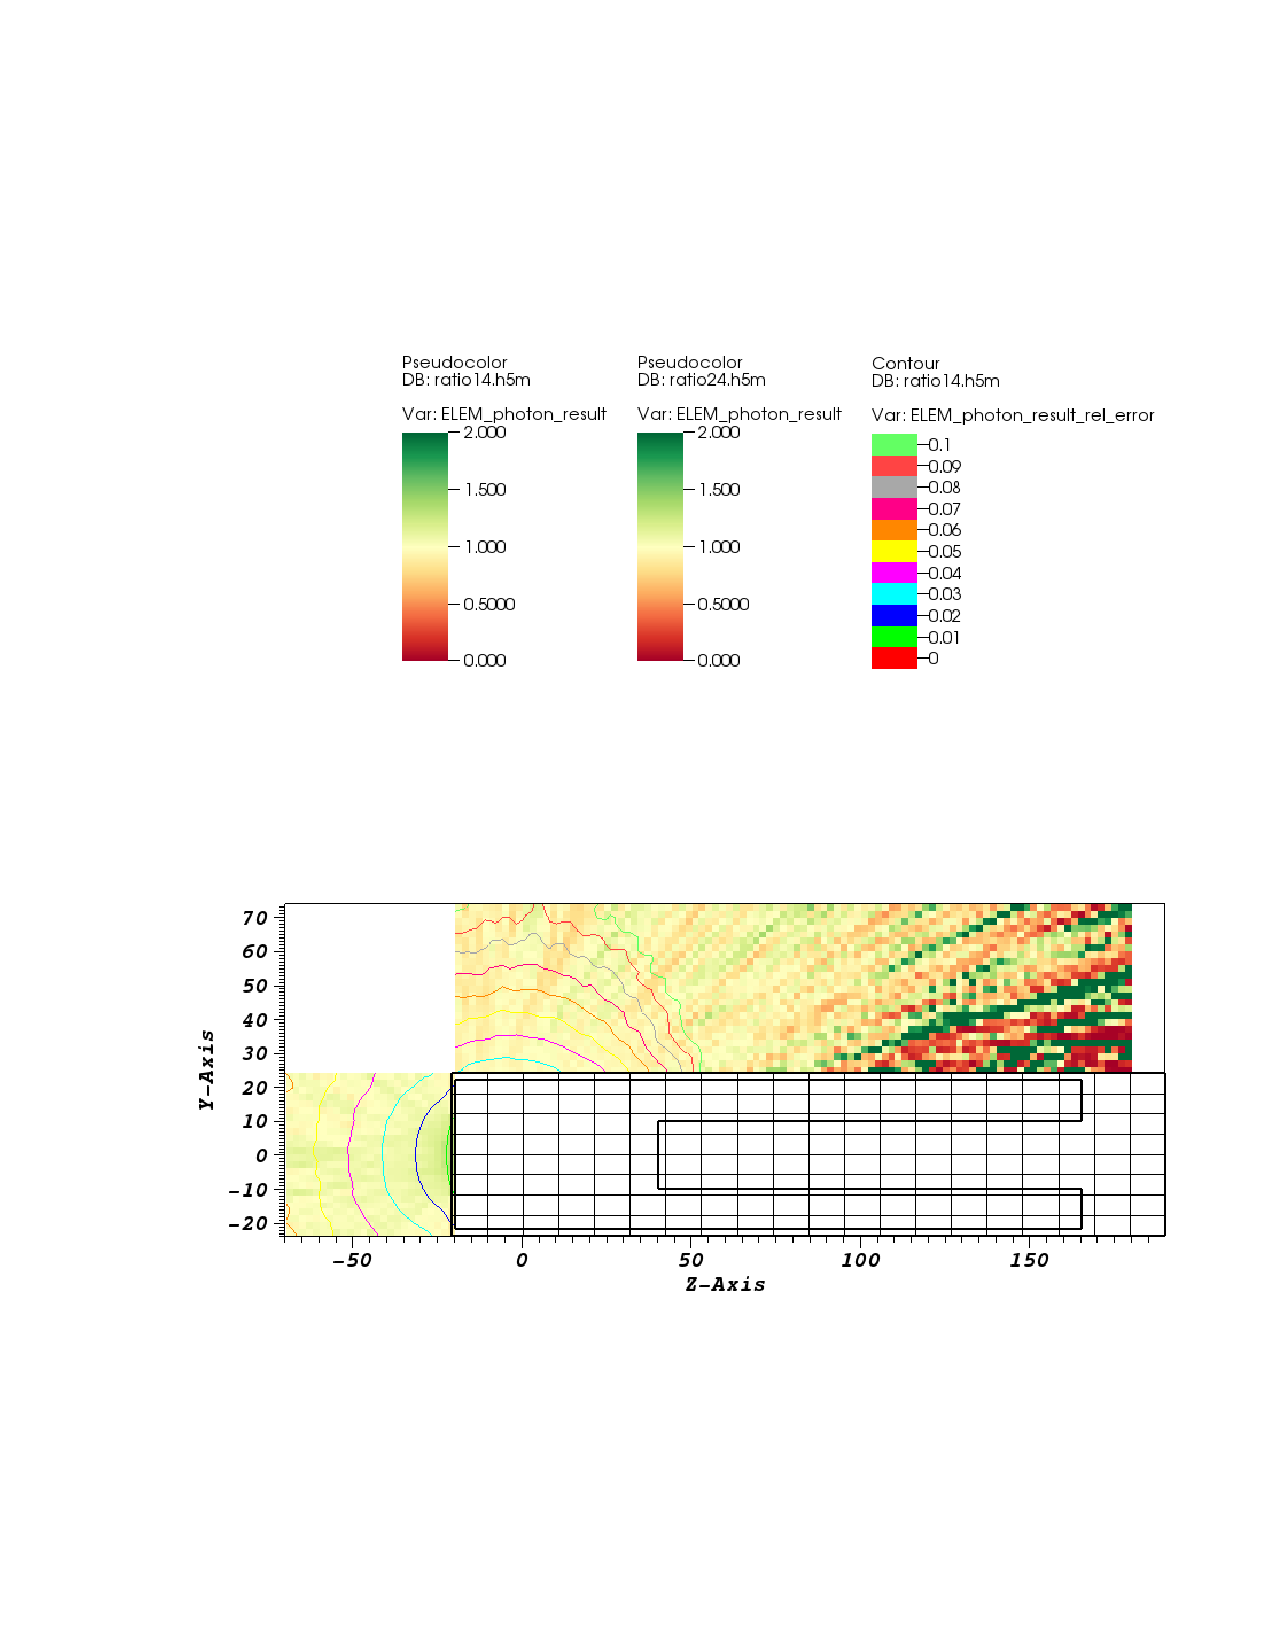
\includegraphics[scale=0.49,trim={6.75cm 16.5cm 11cm 6cm},clip]{figs/ratio_mer_novoid.pdf}
        \end{figure}
	\column{0.1\textwidth}
        \begin{figure}
                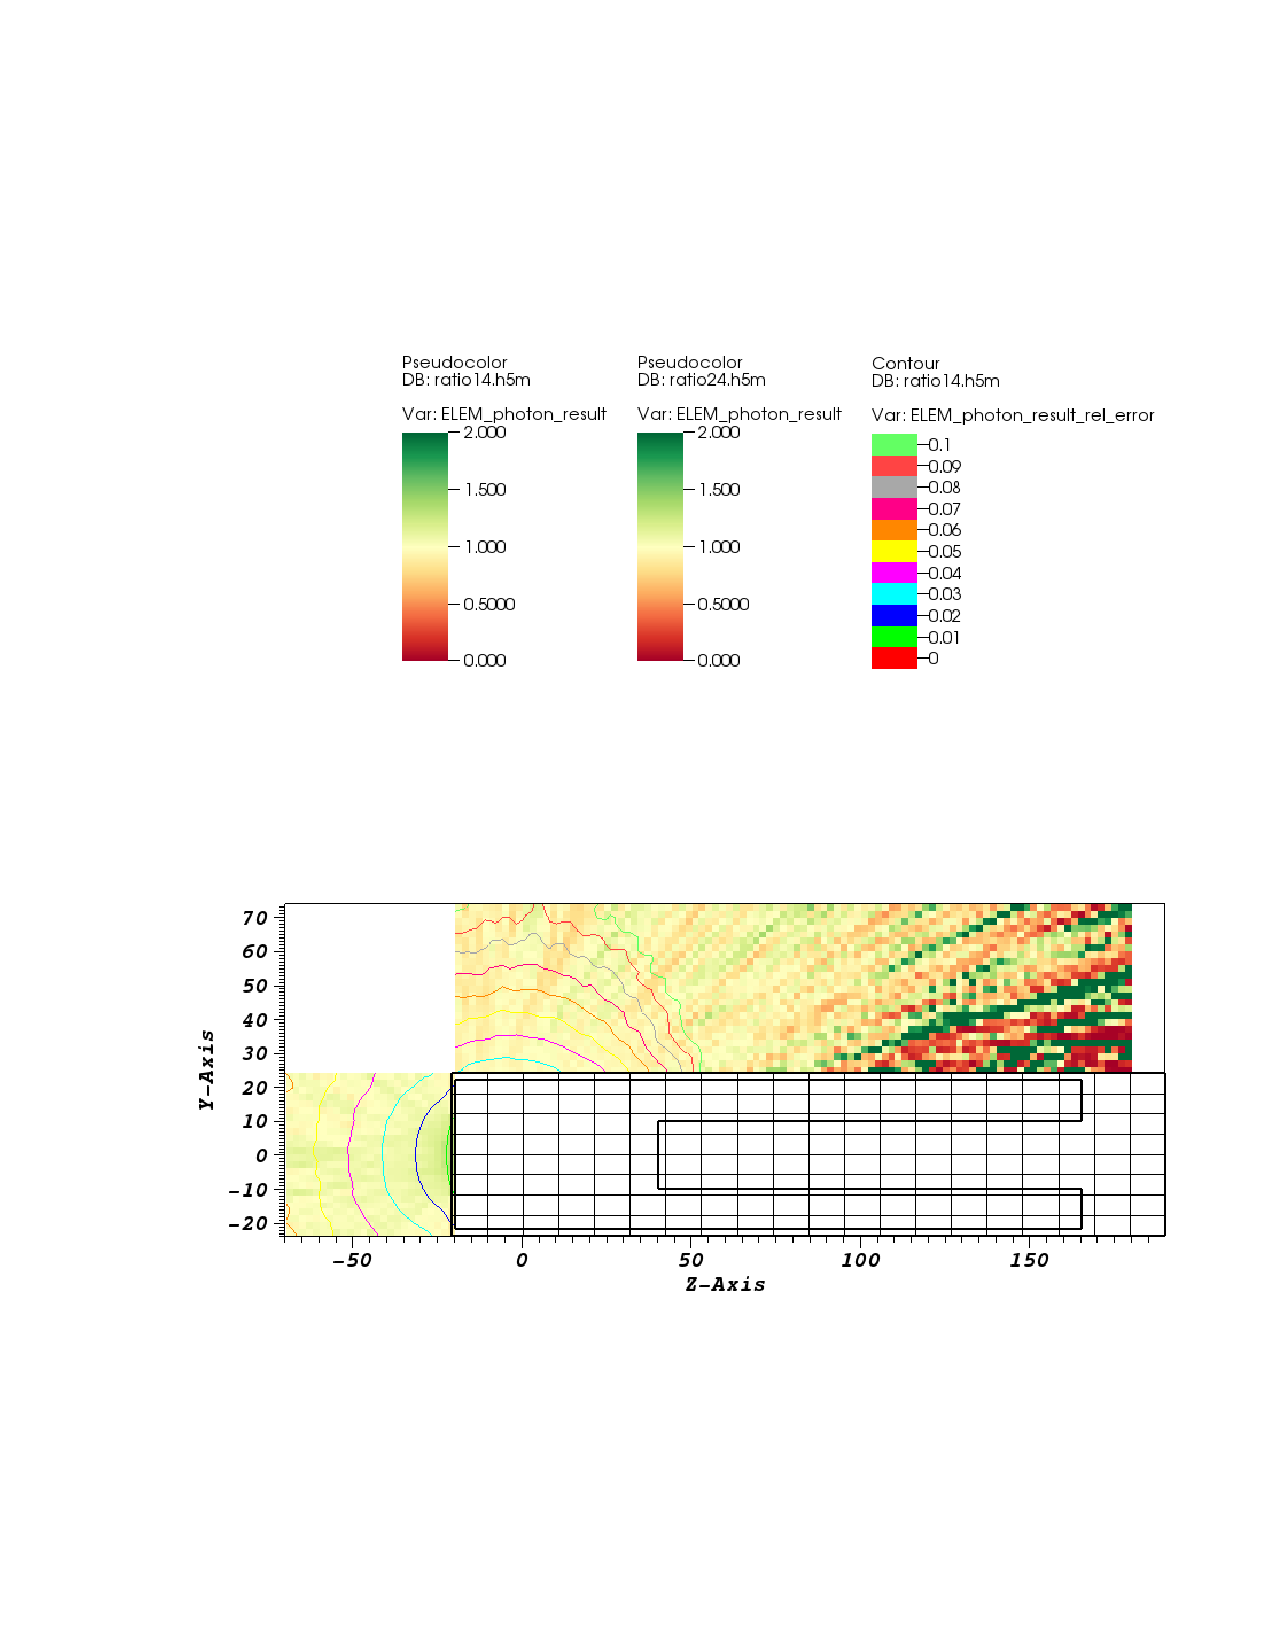
\includegraphics[scale=0.49,trim={20cm 16.5cm 7cm 6cm},clip]{figs/ratio_mer_novoid.pdf}
        \end{figure}

\end{columns}
\end{frame}


%%%%%%%%%%%%%%%%%%%% SLIDE

\begin{frame}{Dose Rates: Steel Source}
\begin{columns}[T]
        \column{0.8\textwidth}
        \textbf{Cell Workflow}
        \begin{figure}
                \centering
                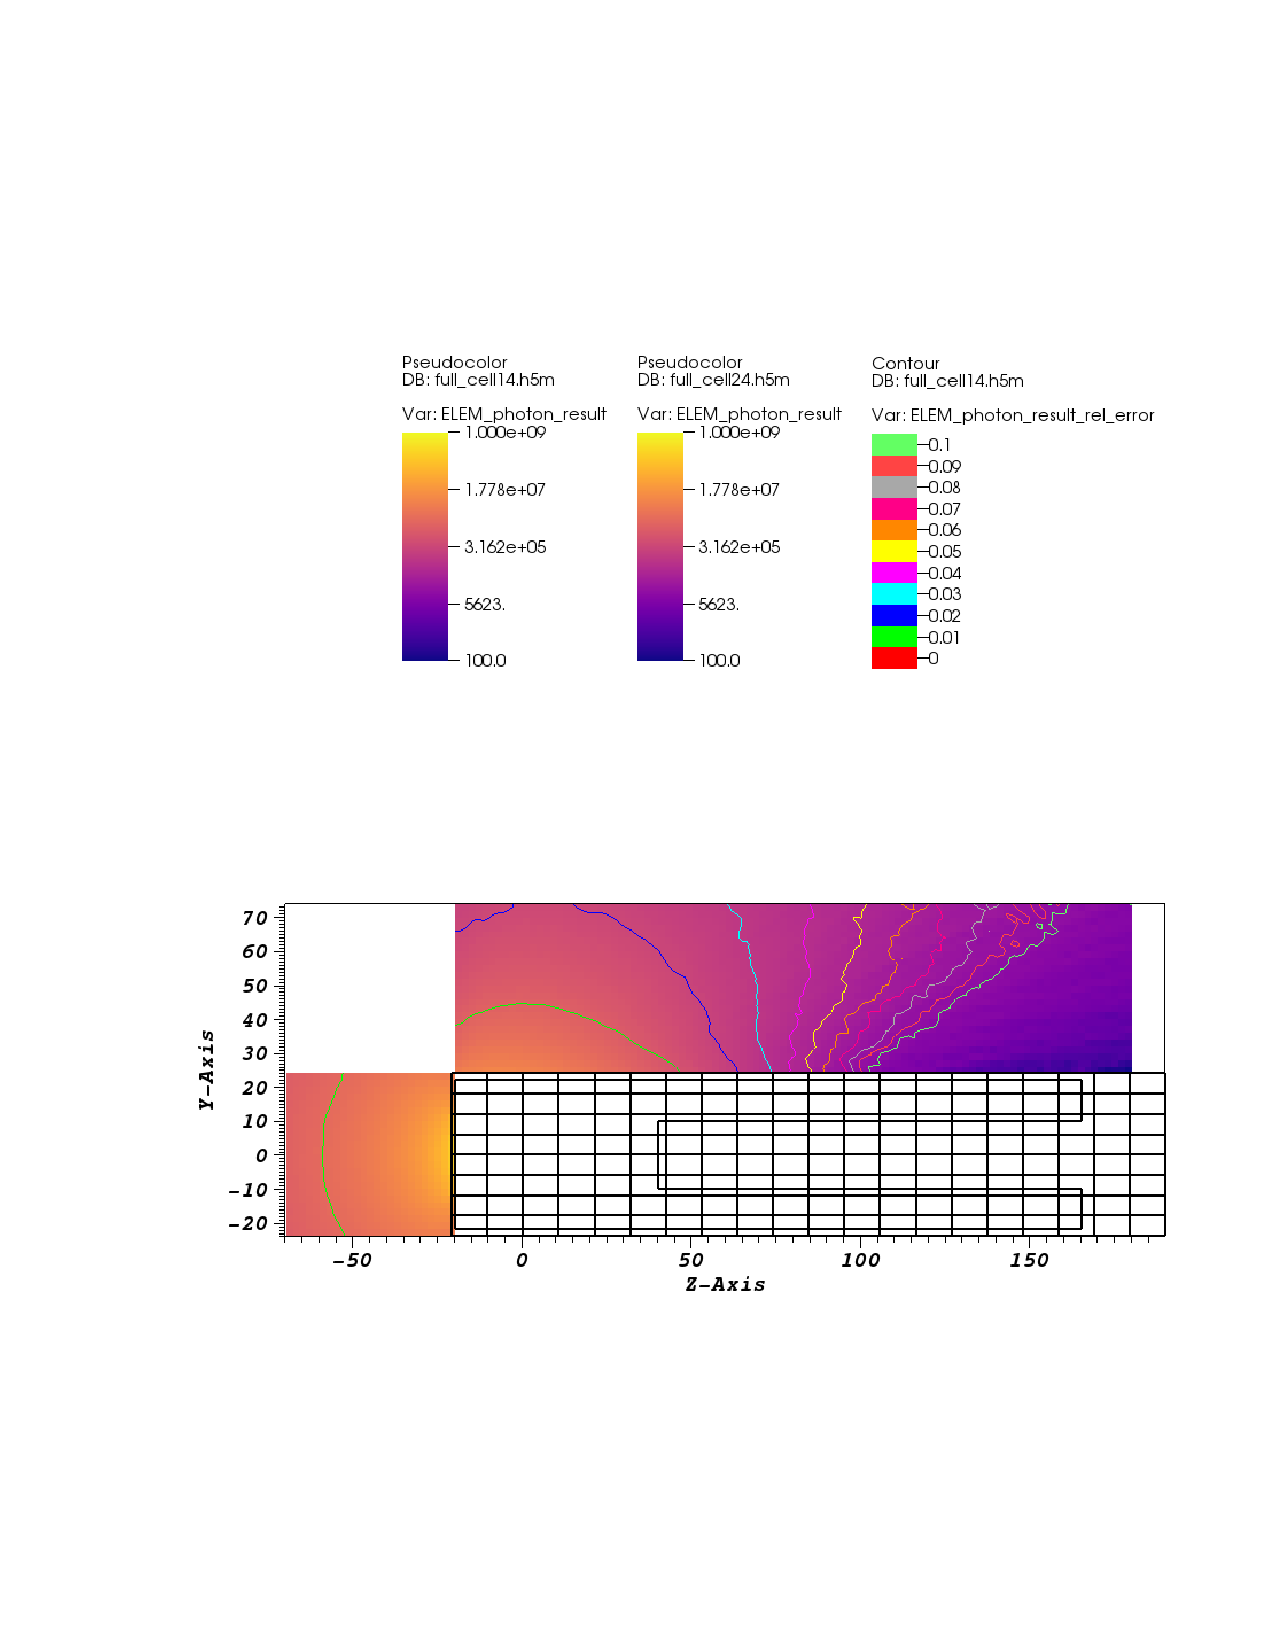
\includegraphics[scale=0.49,trim={2.5cm 6cm 1cm 15cm},clip]{figs/dose_steel_cell_novoid.pdf}
        \end{figure}

        \column{0.2\textwidth}

	\tiny{* thick line = geom} \\
	\tiny{* thin line = src mesh}

        \begin{figure}
                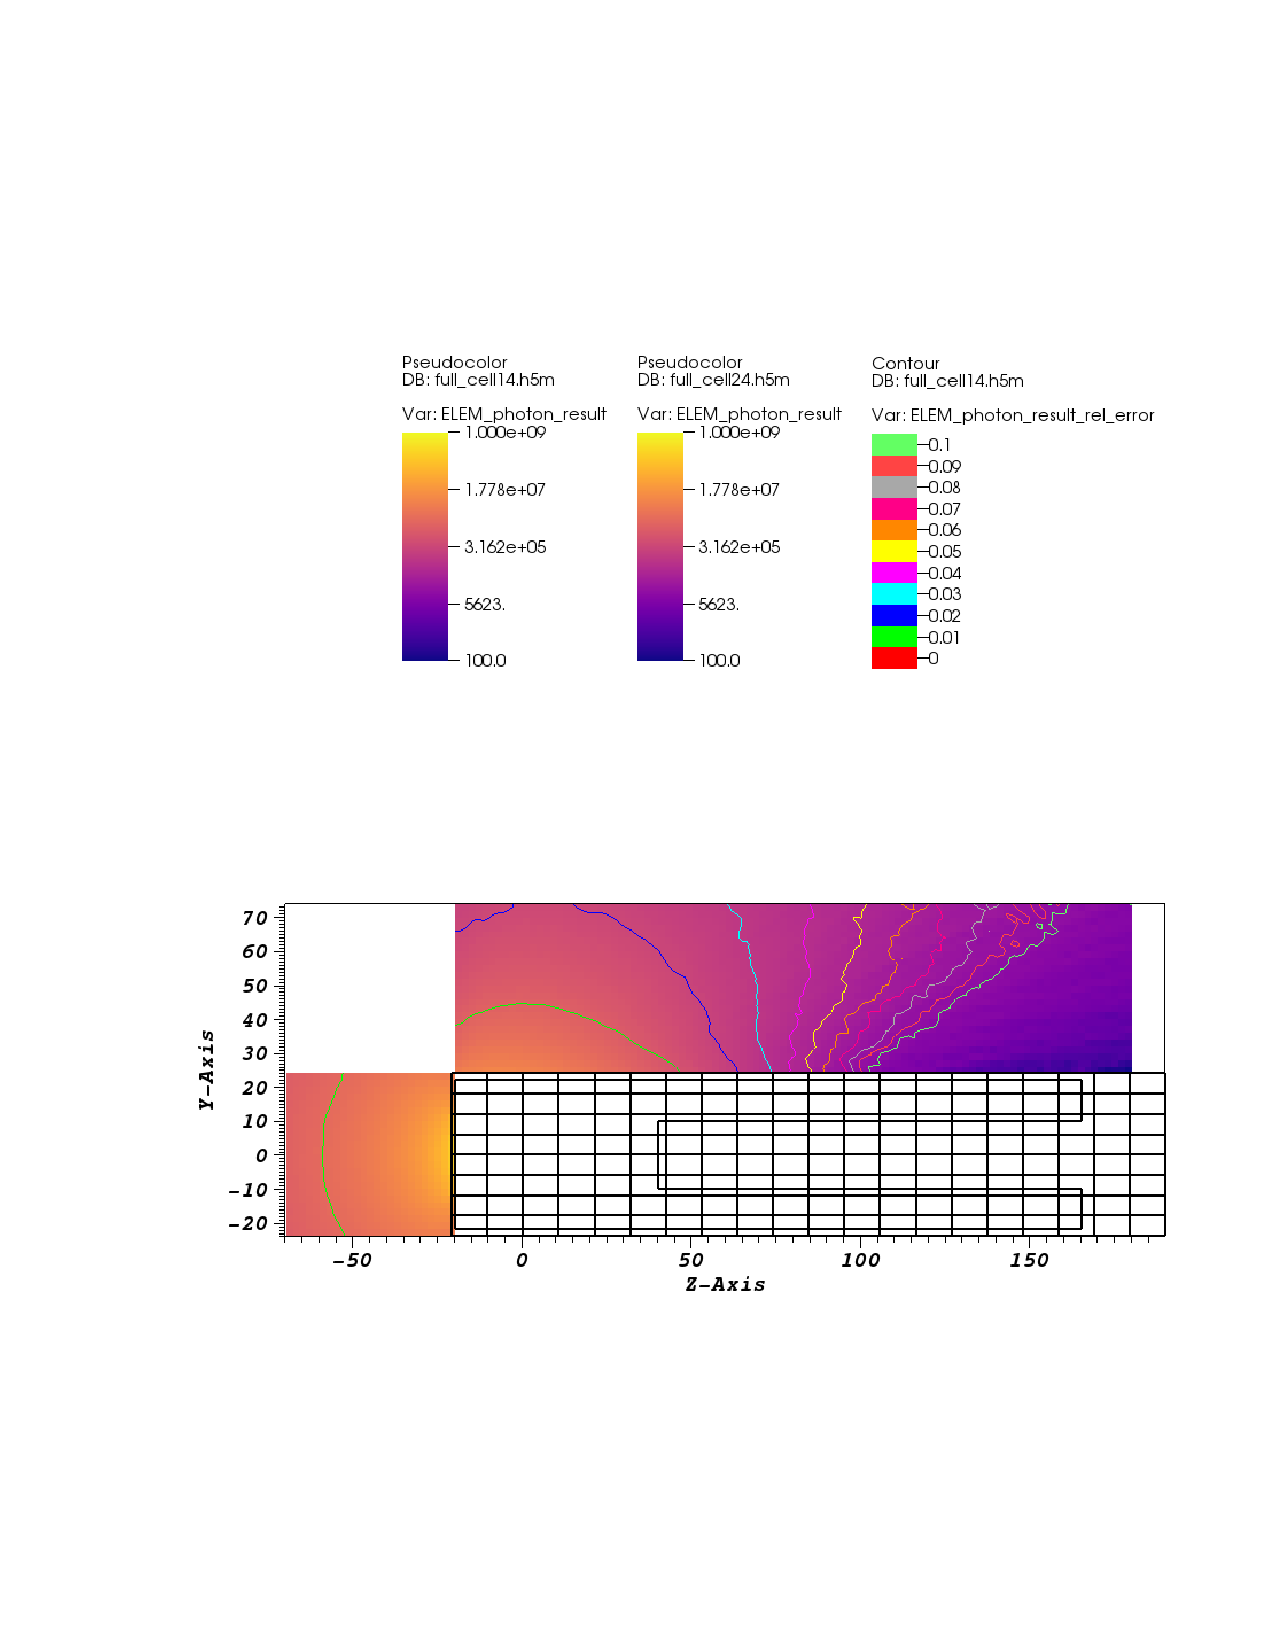
\includegraphics[scale=0.49,trim={6.75cm 16.5cm 11cm 6cm},clip]{figs/dose_steel_cell_novoid.pdf}
        \end{figure}
\end{columns}

\begin{columns}[T]
        \column{0.8\textwidth}

        \textbf{Mesh Workflow}
        \begin{figure}
                \centering
                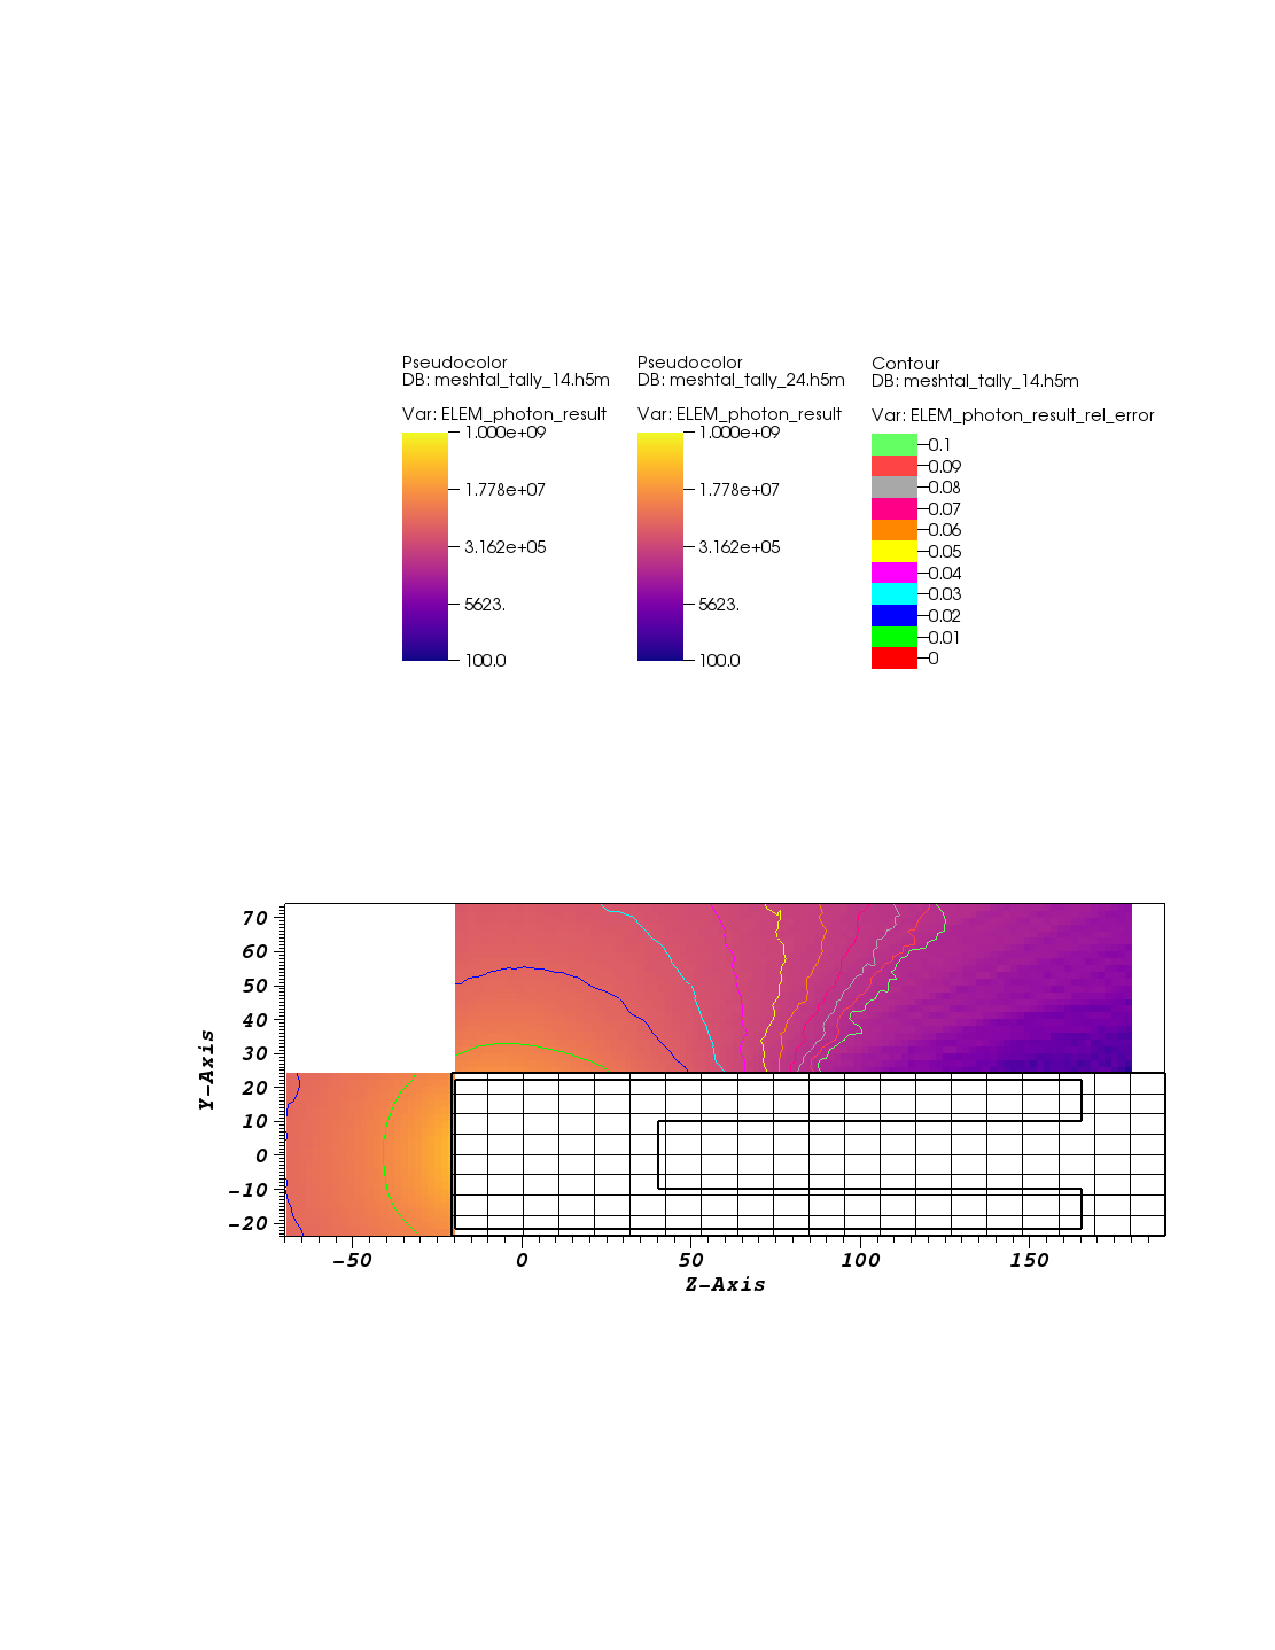
\includegraphics[scale=0.49,trim={2.5cm 6cm 1cm 15cm},clip]{figs/dose_steel_mesh_novoid.pdf}
        \end{figure}

        \column{0.2\textwidth}
        \begin{figure}
                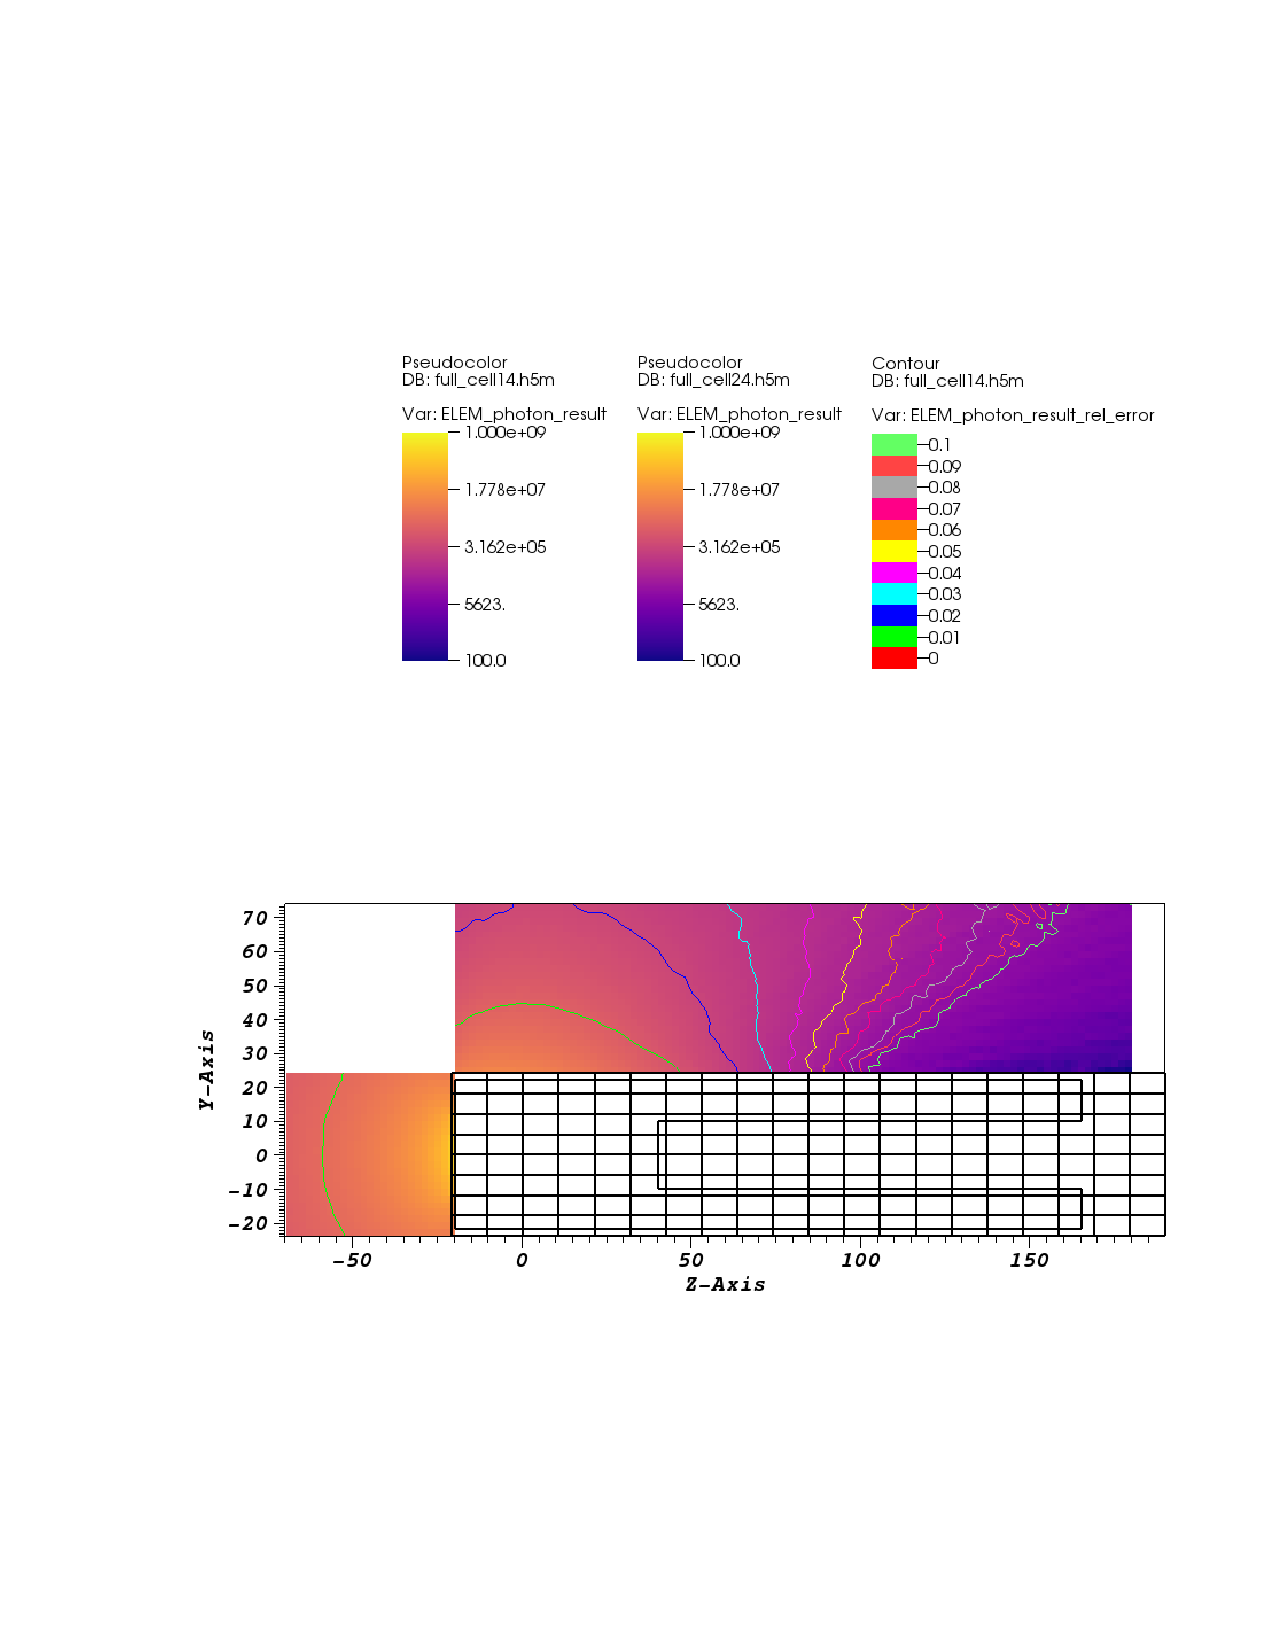
\includegraphics[scale=0.49,trim={20cm 16cm 7cm 5cm},clip]{figs/dose_steel_cell_novoid.pdf}
        \end{figure}

\end{columns}
\end{frame}


%%%%%%%%%%%%%%%SLIDE %%%%%%
\begin{frame}{Dose Ratio: Steel Source}
\begin{columns}[T]
	\column{0.7\textwidth}

        \begin{figure}
                \centering
                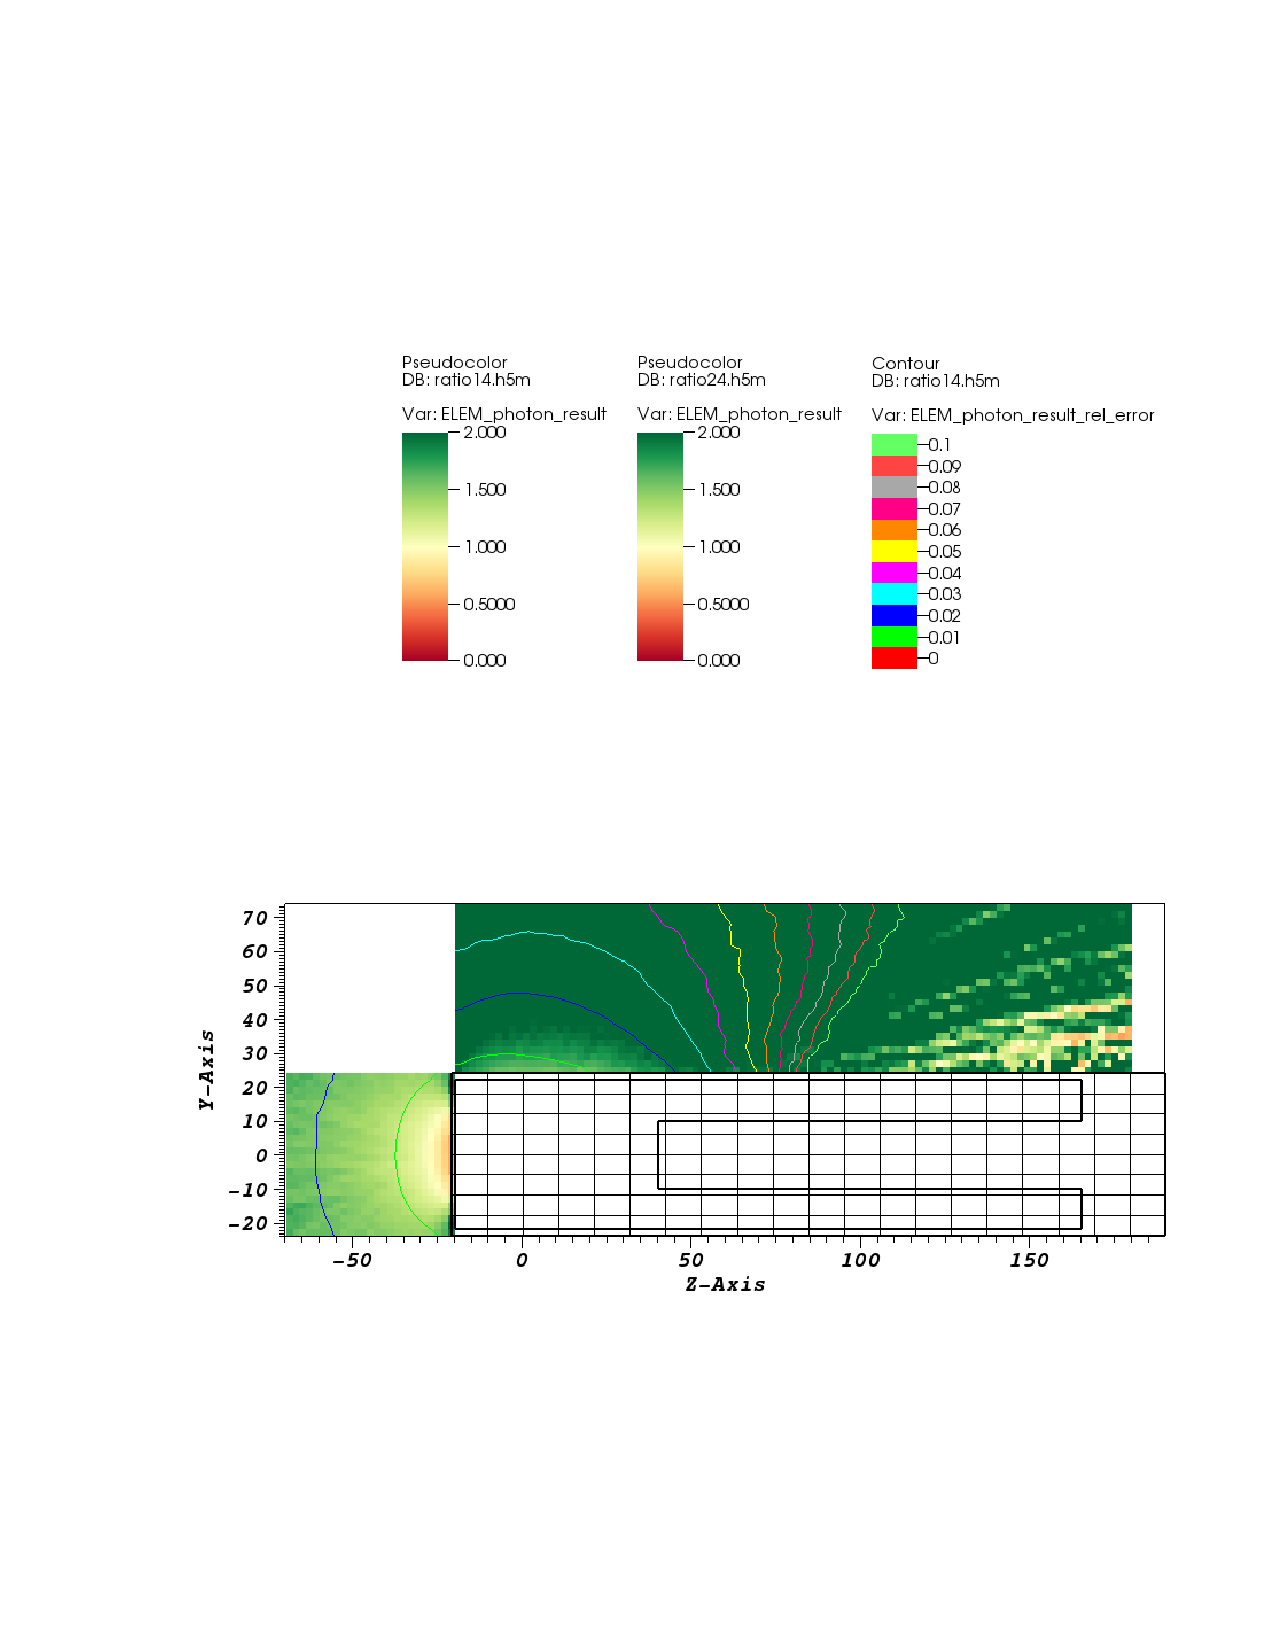
\includegraphics[scale=0.49,trim={2.5cm 6cm 1cm 15cm},clip]{figs/ratio_steel_novoid.pdf}
        \end{figure}

	\column{0.15\textwidth}
        \begin{figure}
                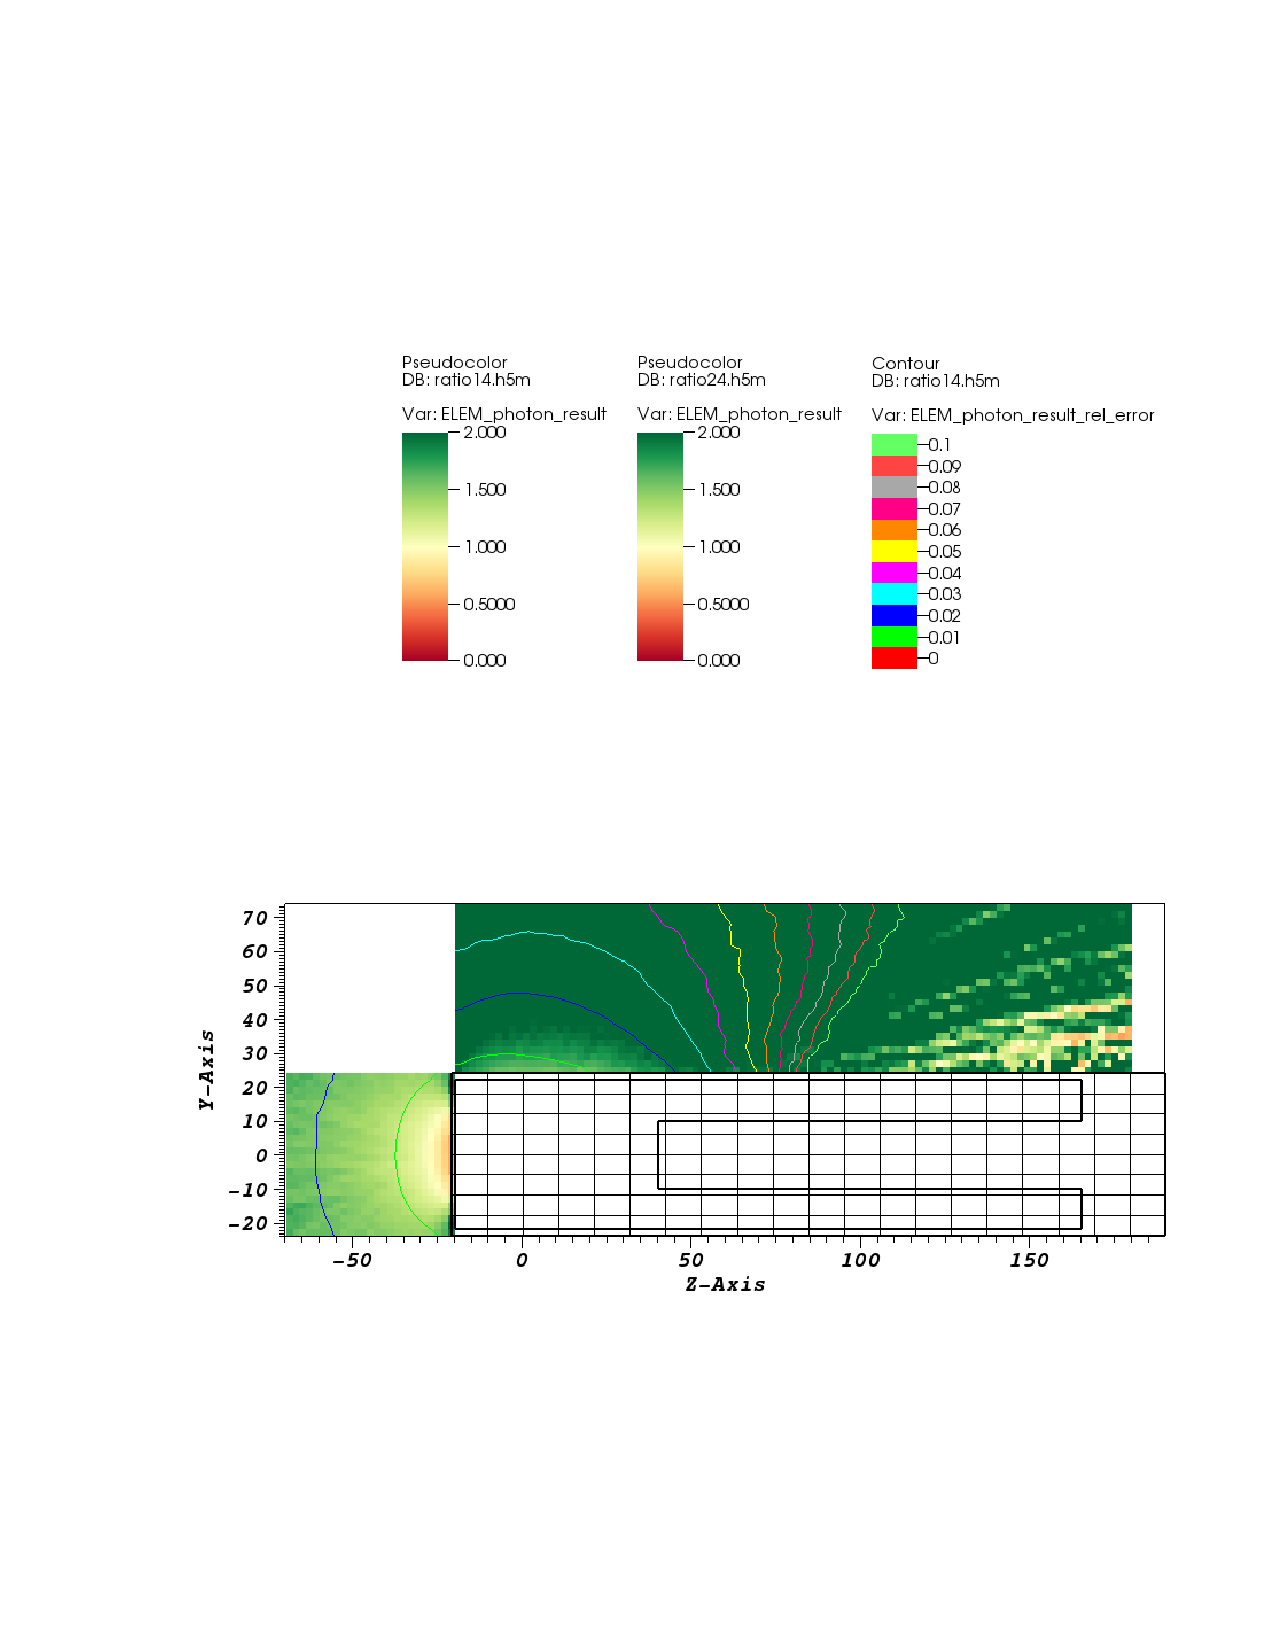
\includegraphics[scale=0.49,trim={6.75cm 16.5cm 11cm 6cm},clip]{figs/ratio_steel_novoid.pdf}
        \end{figure}
	\column{0.1\textwidth}
        \begin{figure}
                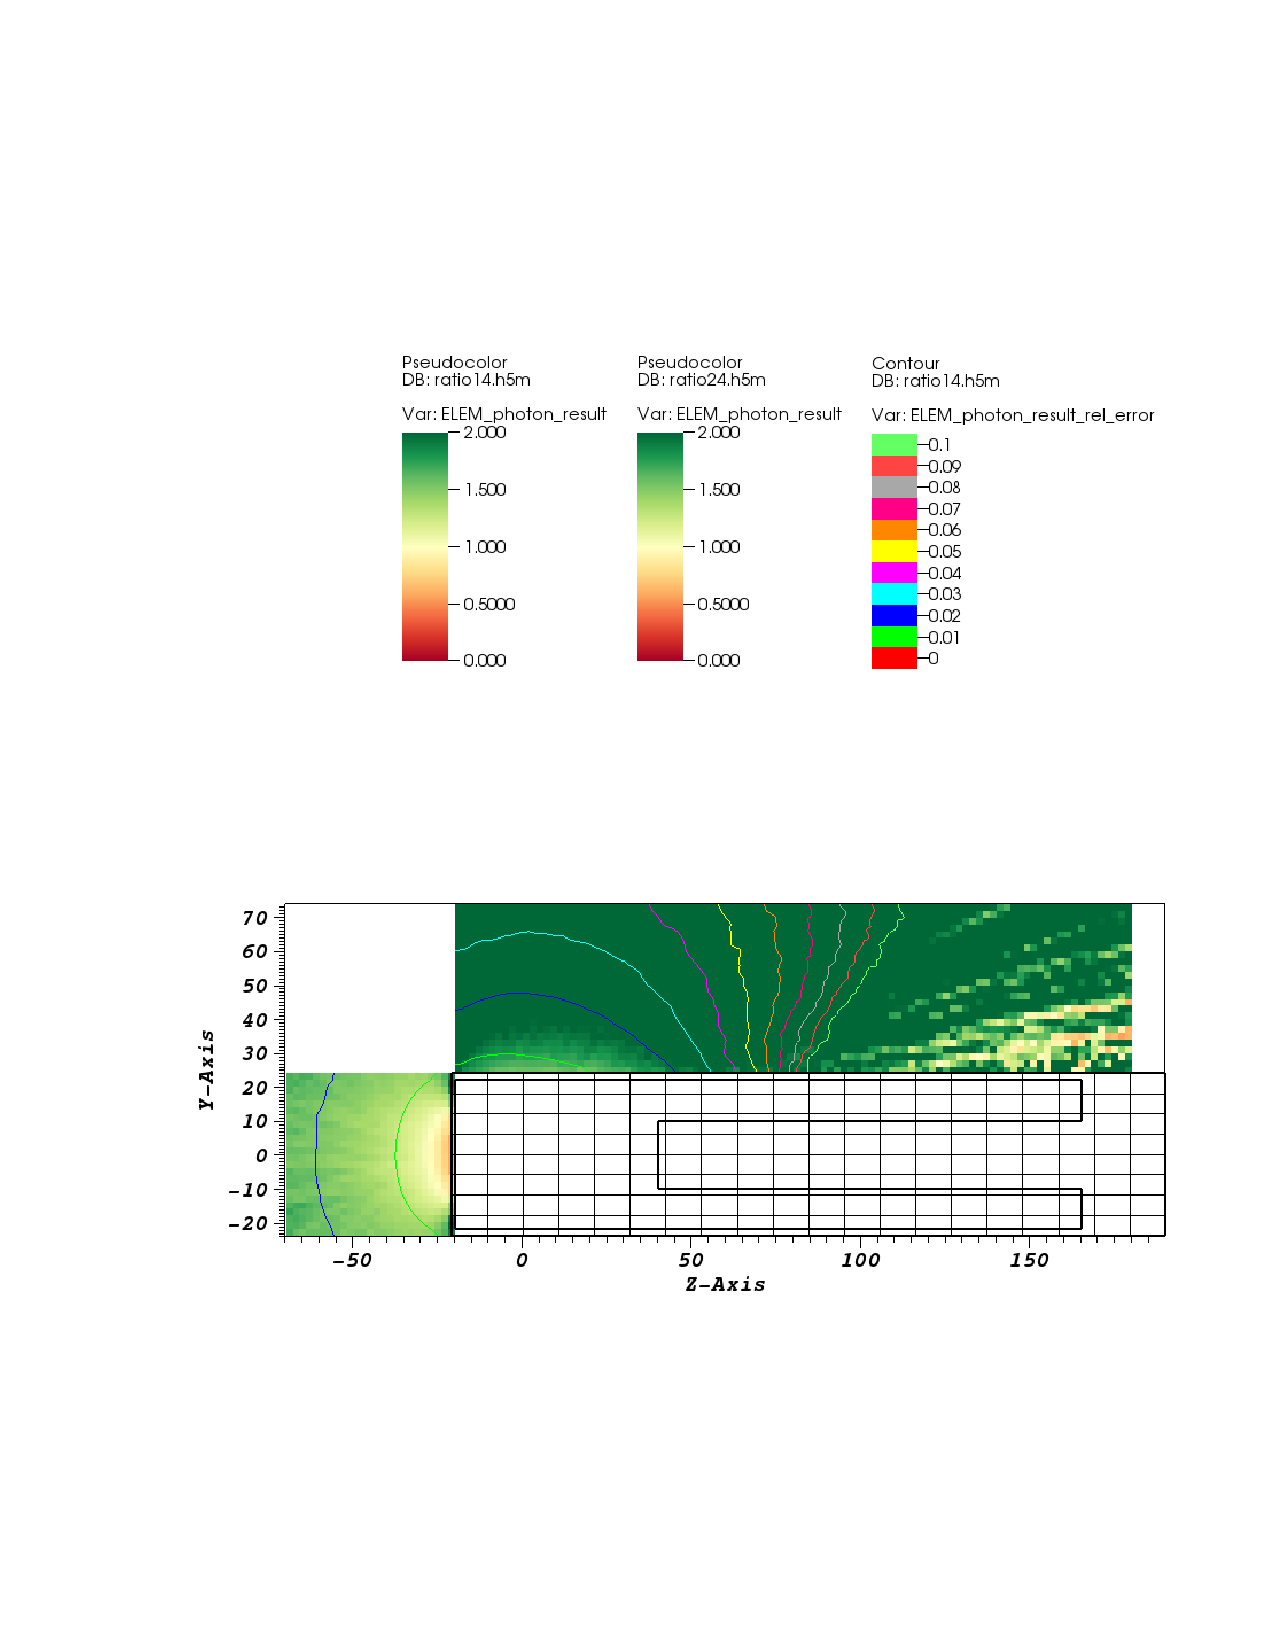
\includegraphics[scale=0.49,trim={20cm 16.5cm 7cm 6cm},clip]{figs/ratio_steel_novoid.pdf}
        \end{figure}

\end{columns}
\end{frame}
\end{document}
